\chapter{探测器组件生产与PSD整体组装}
\label{ch:construction}
相比于地面使用,空间项目对探测器提出了更加苛刻的使用条件和更加严格的质量要求。
这不仅意味着探测器各部件需要进行特殊设计以适应火箭发射过程和空间使用环境,而且探测器组件的生产和整体组装必须遵循一定的建造规范并辅以严格的质量控制程序以保证其达到设计要求和质量。
塑闪阵列探测器的具体设计已经在第\ref{ch:description}章进行了梳理,本章将对它的实际建造过程进行简单介绍。

指导塑闪阵列探测器建造的有两条基本原则:一是要实现其功能要求,二是满足其质量要求。
PSD由探测器主体功能模块,高压扇出模块,前端电子学模块以及机械支撑模块这四部分组成。
其中,高压扇出模块、前端电子学模块和机械支撑模块都由专业的外包单位负责其建造和质量控制,实验室中我们只负责探测器主体功能模块中各探测单元模块的建造,主要包括PMT组件以及塑闪单元条组件。
另外,我们还在实验室中将上述四个功能模块组装成一个整体,最终完成了塑闪阵列探测器的建造工作。

\section{PMT的筛选}
\label{sec:construction:pmt_selection}
PSD由82个探测单元模块组成,并要求它们之间的MIP能量响应一致性好于$\SI{25}{\percent}$。
PSD探测单元模块的MIP能量响应是由R4443的Dy8增益以及塑闪单元条的衰减长度共同决定的。
光电倍增管具有较大的个体差异性,根据上一章\ref{sec:pmt_test:relative_gain}节的测试结果,不同R4443的Dy8增益最大可以相差一个量级;
而对于塑闪单元条来说,不同衰减长度导致的光输出差异最大不超过\SI{30}{\percent}(见\ref{sec:construction:bar_production}节的结果)。
因此,选择性能参数相近的R4443管子对保证探测单元模块的一致性尤为关键。
我们把PSD中PMT的筛选过程提取出来单独作为一节,对其进行详细描述。

首先,我们对所有待选的R4443管子进行了质量筛选,主要有:1)根据Hamamatsu提供的出厂测试参数淘汰阳极暗电流过大和工作状态稳定性(Drift,见\parencite{hamamatsu})较差的管子;2)淘汰尺寸超过标准误差以及光阴极和外观有瑕疵的管子,由于PMT组件装配时对R4443的尺寸具有严格要求,因此我们在实验室对所有R4443裸管的尺寸进行了测量,另外我们还对管子的光阴极和玻璃管体表面进行了细致的检查以排查有细微裂纹的管子;3)淘汰参加了出厂前力学检测的管子,我们要求Hamamatsu随机抽取部分该批次的R4443管子进行振动和冲击测试,测试结果证明了R4443的力学性能够满足PSD的设计要求,但出于保守考虑,这些经历了力学测试的管子将不会安装到PSD探测器上。
这轮筛选中被淘汰的管子数量并不多,而且它们虽然不能够满足PSD的质量要求,但仍能在地面项目中继续使用。

之后,我们基于R4443的增益特性曲线与Dy58比值特性曲线,依照增益与动态范围两个方面的需求进行了一步的筛选,淘汰了具有极端特性的管子并确定了被选管子的工作电压档位。
第\ref{ch:pmt_test}章得到的Dy58比值特性曲线是绝对测量的结果,因此可以直接使用;
而得到的Dy8增益特性曲线是相对测量的结果(详见\ref{sec:pmt_test:relative_gain}节),不能直接使用。
为了在PSD的PMT筛选过程中使用该曲线,我们以某中一只管子的真实MIP响应为参照来计算其它所有管子的MIP响应,原理如下:
\begin{enumerate}
	\item 从待选管子中任选一支R4443,我们将其称为$PMT_{ref}$,$PMT_{ref}$与其它所有待选管子一样,在第\ref{ch:pmt_test}章中已经得到了它的增益特性曲线。
	\item 从待选的塑闪单元条中选取一根衰减长度在均值附近的条子,并将它与$PMT_{ref}$耦合成PSD的探测单元模块。该单元模块的另一端也耦合上PMT以保证其结构与实际情况完全一致,并且模块的装配和使用的材料也与实际使用的完全一致。
	\item 使用宇宙线对该单元模块中心位置处的MIP响应进行测试,考察$PMT_{ref}$对MIP入射光强$L_{mip}$的响应。通过调节$PMT_{ref}$的电压,我们将它的MIP响应中心值移到到设计值附近,令这个值为$A_{mip}$。这个工作电压就是$PMT_{ref}$的最佳工作电压,而此时的$PMT_{ref}$增益就是我们的参考增益,我们期望其它管子也工作在这个增益下。
	\item 为方便计算,我们没有使用以$G_{relative}$表述的相对增益测试结果,而是直接使用了以$A_{corr}$表述的结果,即增益特性曲线中没有消去入射光强量(详见\ref{sec:pmt_test:relative_gain}节)。我们选取了最弱入射光强(令其强度为$L_{test}$)测得的Dy8增益特性曲线,并计算出最佳工作电压下$PMT_{ref}$对该光强的响应中心值为$A_{test}$。
	\item $A_{test}$与MIP响应最佳值的比值,就是测试用的入射光强与实际的MIP入射光强的比值,即
	\begin{equation}
		\frac{A_{mip}}{A_{test}} = \frac{L_{mip}}{L_{test}}
		\label{eq:construction:pmt_selection}
	\end{equation}
	由上式可以推得$A_{mip}=A_{test}L_{mip}/L_{test}$,这意味着:如果其它管子在$L_{test}$入射光强下的响应中心值也为$A_{test}$,则它们耦合到塑闪单元条上后对MIP的响应中心值就是我们期望的设计值$A_{mip}$,而此时的增益就是最佳增益。
	由于我们已经得到了所有管子在$L_{test}$入射光强下的增益特性曲线,因此可以根据$A_{test}$值反推出各个管子的最佳工作电压。
\end{enumerate}
实际筛选中,$A_{mip}$被确定为450道,而我们选择的参考PMT所对应的$A_{test}$值在700道左右。

DAMPE高压单机只能提供不连续的高压档位且档位间隔为\SI{30}{V},而PSD只有7个工作电压档位可以使用(见\ref{sec:description:psd_hv}节)。
这极大限制了PSD的PMT筛选,我们只能尽量选择这样一些管子,使得它们的额定工作电压档位与最佳工作电压值尽量接近。
为了保留档位调节的余地,我们以\SI{810}{V}、\SI{840}{V}、\SI{870}{V}和\SI{900}{V}这四个档位为额定工作电压档,具体的筛选流程如下:
\begin{enumerate}
	\item 淘汰具有极端增益的管子。根据最小入射光强得到的Dy8增益特性曲线,计算每个管子对应于$A_{test}$时的工作电压,淘汰最佳工作电压在$\SI{790}{V}\sim\SI{900}{V}$范围外的管子。
	\item 确定额定工作电压。根据最小入射光强得到的Dy8增益特性曲线,分别计算SI{810}{V}、\SI{840}{V}、\SI{870}{V}和\SI{900}{V}四个电压档位下的响应中心值$A_{real}$,淘汰所有四个$A_{real}$值都在区间$[A_{test}-100,A_{test}+100]$范围外的管子。如果只有一个电压档位下的$A_{real}$值在该区间内,则这个档位就是该PMT的额定工作电压档位;如果多个电压档位下的$A_{real}$值在该区间内,则该PMT的额定电压由后面的筛选步骤确定。大部分管子在这一步就确定了额定工作电压档位。
	\item 淘汰动态范围不合适的管子。根据下面的公式可以计算出额定工作电压下各管子的动态范围上限$D_{range}$:
	\begin{equation}
		D_{range} = 12000\cdot G_{58} / (A_{mip}\cdot \frac{A_{real}}{A_{test}})
		\label{eq:construction:dynamic_range}
	\end{equation}
	其中,$12000$是Dy5通道的有效线性范围,$G_{58}$是根据Dy58比值增益曲线计算出的该管子在额定工作电压下的Dy58比值,而其它符号的定义同之前的定义一样。
	我们淘汰了$D_{range}$在区间$[1200,1400]$范围外的管子。
	\item 淘汰Dy8增益随电压变化异常的管子。DAMPE设计寿命为3年。由于寿命的原因,在DAMPE运行后期,PSD塑闪单元条的光产额和光电倍增管的增益都有可能减小,此时需要提高R4443的工作档位以保持PSD的探测性能不发生重大变化。因此,我们计算了提高三个档位后,即在额定工作电压值上再加90V后,R4443的Dy8增益相对于原来的比值,并淘汰了计算结果在区间$[1.6,2]$范围外的管子。这样就能保证提高工作电压档位后,PSD各探测单元模块间的一致性也会不发生巨大变化。
\end{enumerate}

经过上述两轮筛选过程,我们最终从570支R4443裸管中挑选出了190支管子,并确定了它们的额定工作电压档位。
这些管子将会经历完整的PMT组件生产流程(详见\ref{sec:construction:pmt_procedure}节),其中的164支最终会被安装到PSD探测器上,额外的26支管子将作为备份,以防组件生产过程出现的意外情况(如PMT损伤,PMT组件质量不合格等等)。

\section{PMT组件的生产}
\label{sec:construction:pmt_production}

\subsection{PMT组件的结构简介}
\label{sec:construction:pmt_assembly}
一个完整的PMT组件包括:R4443裸管,Base电路板,EJ-560硅脂垫片,铝合金保护套,高压和信号线缆。
为了更好地保护PMT组件,我们使用室温硫化硅橡胶(RTV胶)将R4443裸管、Base电路板以及硅脂垫片这三部分灌封在一个硅胶保护套中,以减弱火箭发射时产生的剧烈振动和冲击对各部件的影响。
硅胶保护套可以分为两段,分别由不同的材料组成:
\begin{itemize}
	\item 避光部分。PMT是光敏器件,虽然PSD的机械结构设计是密封不透光的,为了以防万一,我们还是给光电倍增管设计了专门的避光措施。这部分胶体覆盖整个R4443裸管和硅脂垫片,并将它们连为一体。它由黑色材料构成,可以有效屏蔽外界光干扰。
	\item 绝缘部分。PSD分压器在工作时需要加载近千伏的高压,而太空中空气密度极低,再加上Base电路板的设计紧凑,板上各元器件间的距离较近,这些都大大增加了电晕放电甚至高压击穿的概率。这部分胶体与前面的避光胶体部分紧密粘连,并完满填充了Base电路板上元器件间的空间。它由绝缘材料组成,从而能够有效防止分压器电路在真空中的高压打火,保护元器件不受损伤。
\end{itemize}
图\ref{fig:construction:pmt_assembly}给出了一个灌封完成后的完整PMT组件照片,它是PMT组件安装到PSD前的最终状态。
%其中的信号接头和高压接头是为了方便生产过程中的质量测试临时焊接上去的,正式安装时会减去这些接头,将高压信号电缆直接焊接到高压扇出板和信号转接板上。
\begin{figure}[htbp]
	\centering
	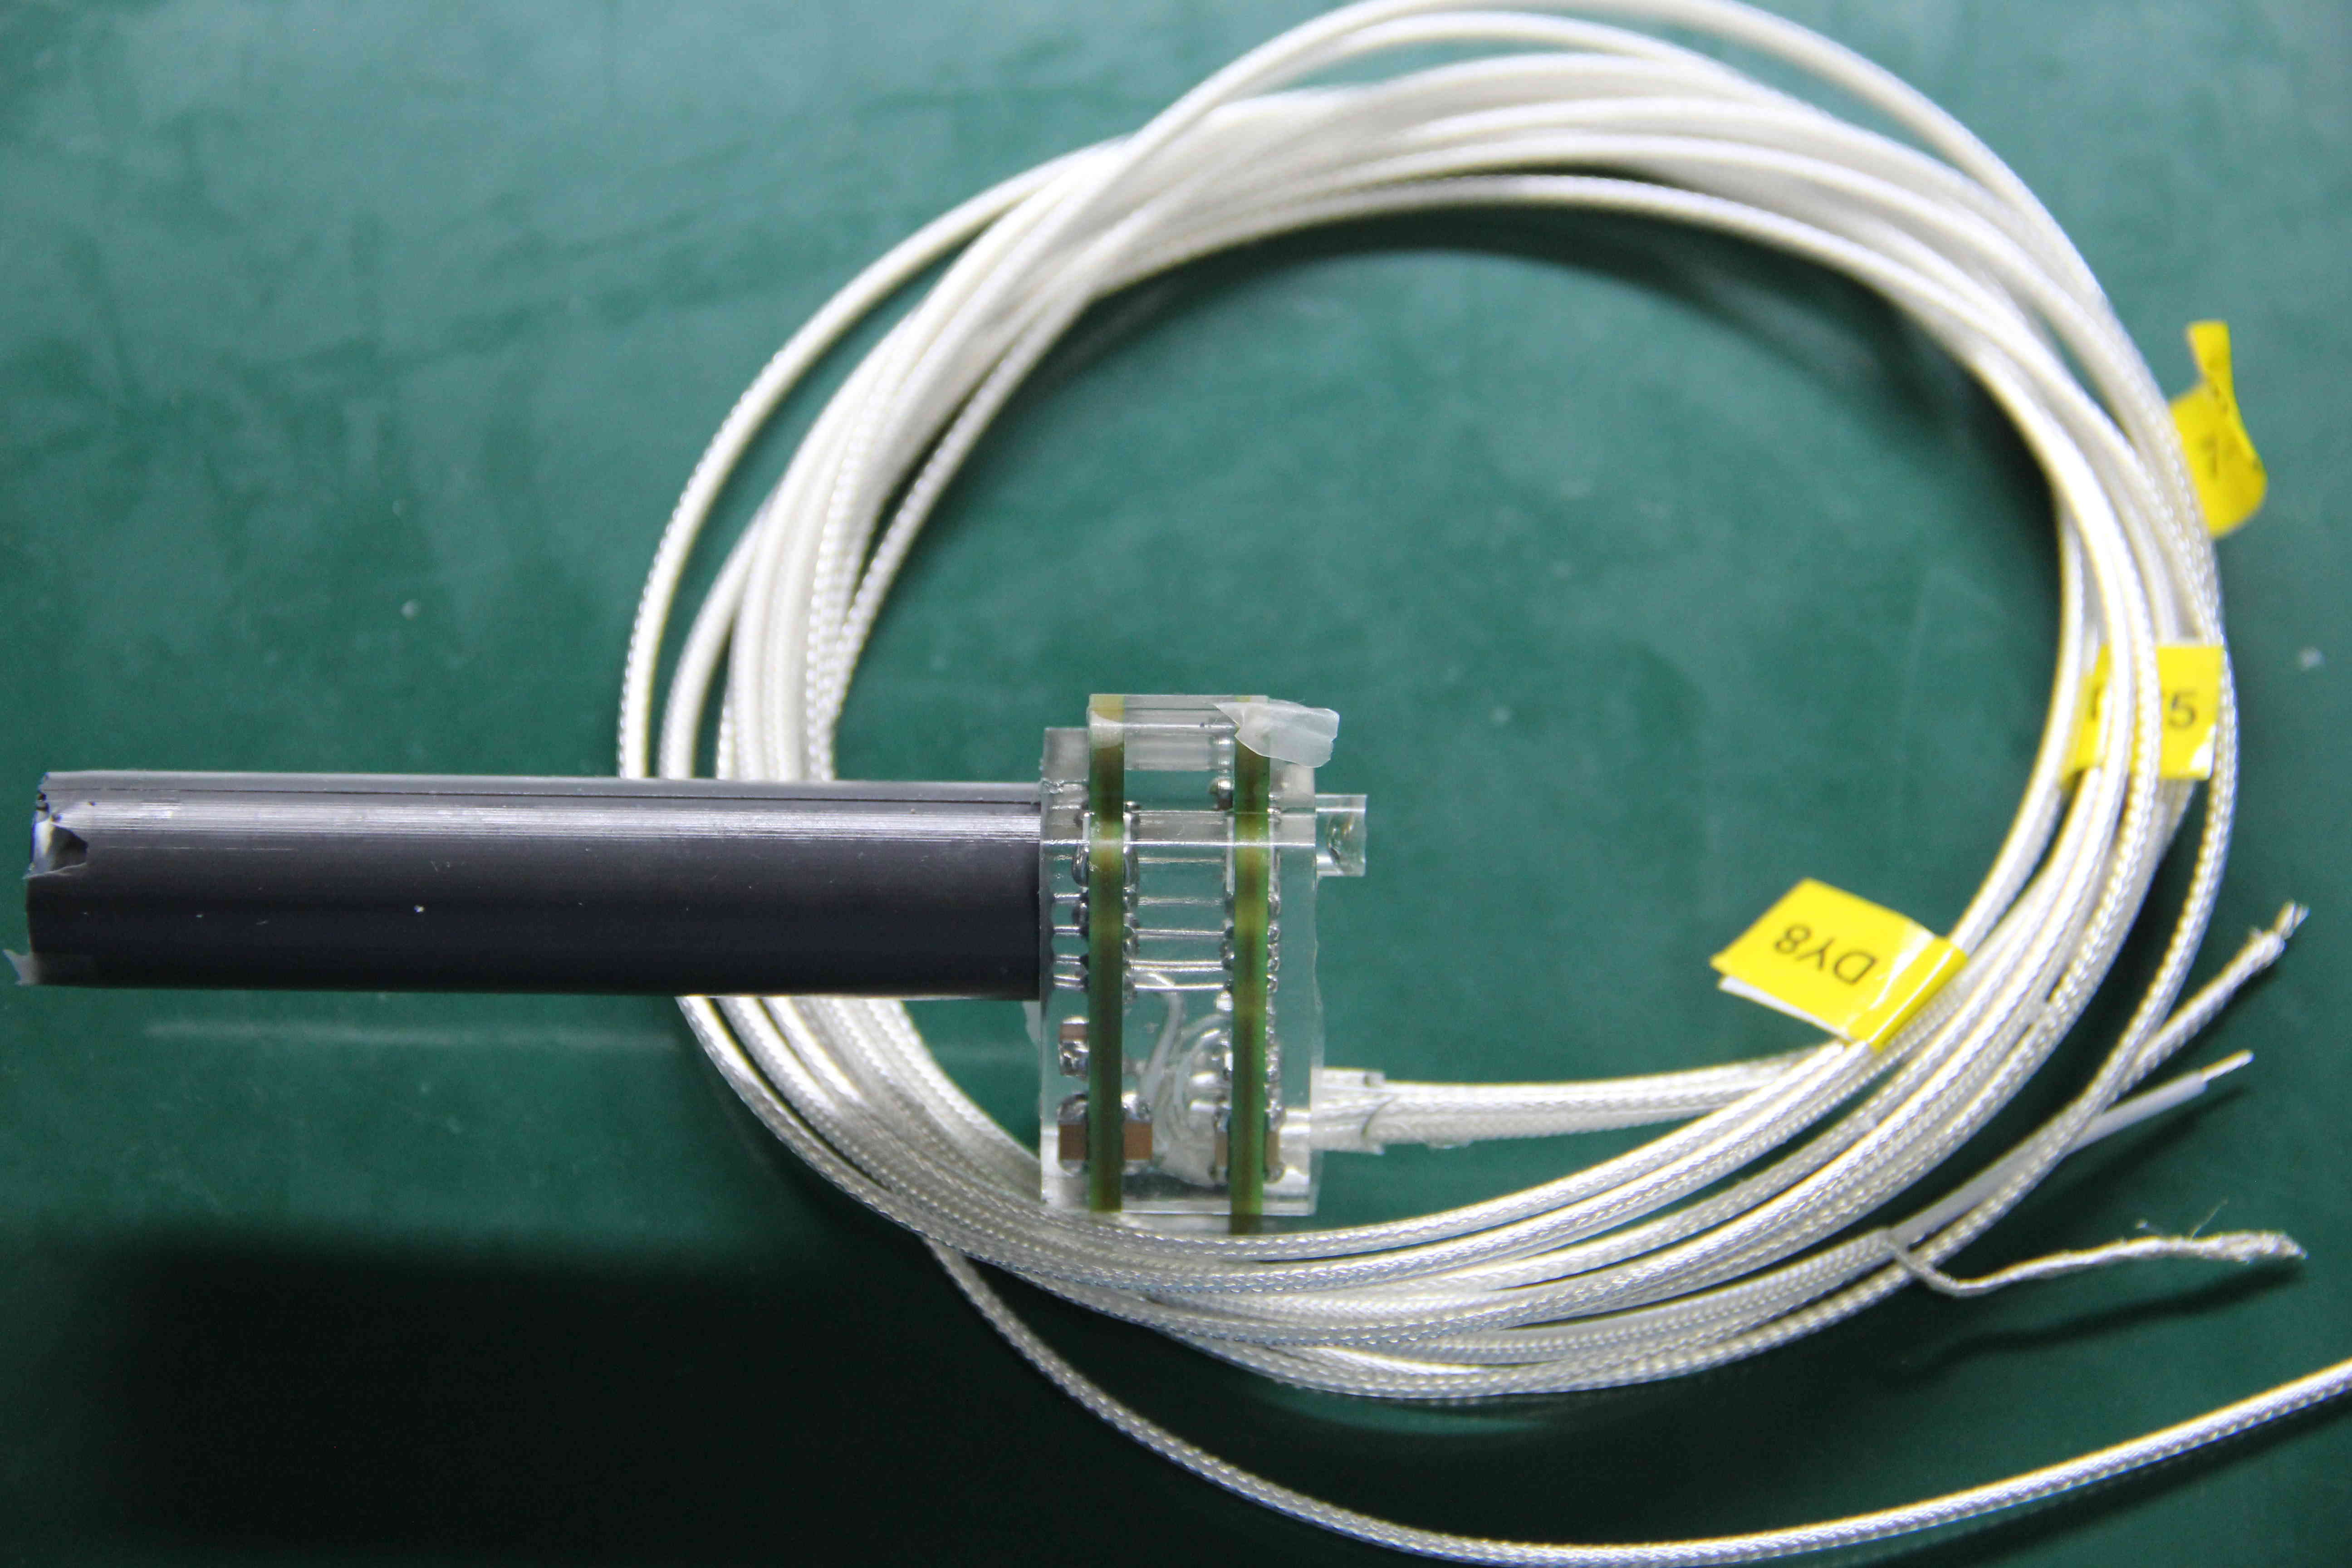
\includegraphics[width=0.65\textwidth]{chap/construction/fig/pmt_assembly.jpg}
	\caption{一个完整的PMT组件}
	\label{fig:construction:pmt_assembly}
\end{figure}

\subsection{PMT组件的生产流程}
\label{sec:construction:pmt_procedure}
PMT组件的整个生产流程可以归纳为四个阶段,按先后顺序依次为为PMT的性能测试和筛选(Selection),PMT组件的生产(Production),PMT组件的环境试验(Environment Test)以及PMT组件的质量鉴定测试(Qualification),如图\ref{fig:construction:pmt_production_procedure}所示。
其中,PMT的性能测试和筛选已经在前面的章节中进行了介绍,这里主要对剩下的三个阶段进行一个梳理。
\begin{figure}[htbp]
	\centering
	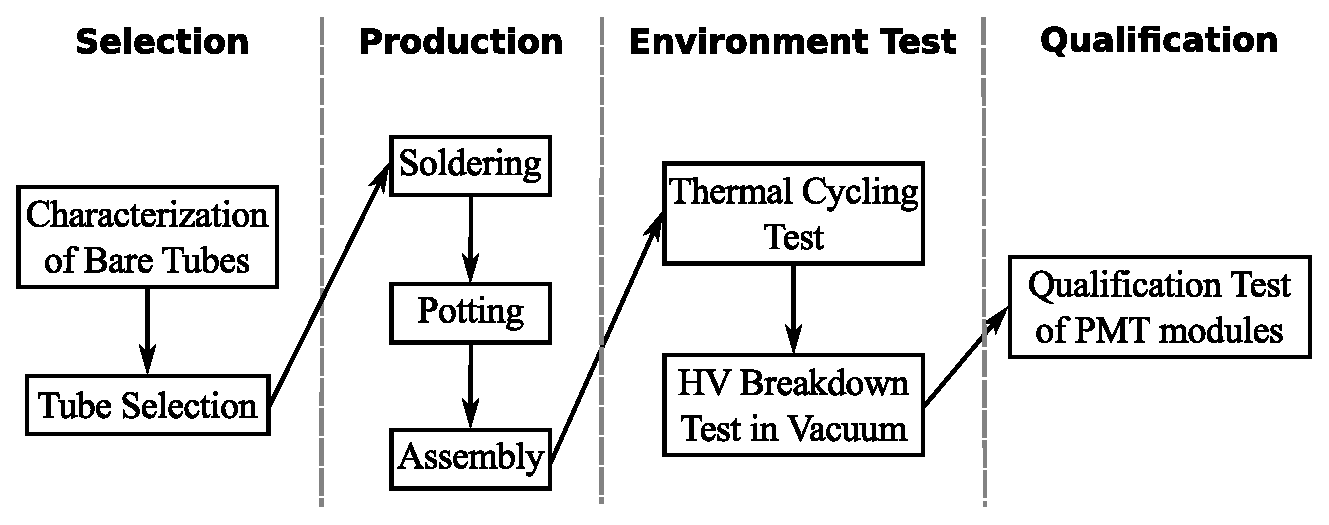
\includegraphics[width=0.95\textwidth]{chap/construction/fig/pmt_production_procedure.eps}
	\caption{PMT组件的生产流程}
	\label{fig:construction:pmt_production_procedure}
\end{figure}
 
% production phase
PMT组件的生产包含三个步骤:Base电路板焊接(Soldering),PMT组件灌封(Potting)和PMT组件装配(Assembly)。
Base电路板焊接是指将R4443裸管与Base的分压器电路板焊接到一起。
由于后面的灌封流程以及PSD的整体装配对PMT组件的尺寸大小具有严格的要求,我们设计了专门的焊接支架用来控制PMT管身与Base电路板之间以及两块Base电路板自身之间的距离。
焊接工作由来自山东航天电子技术研究所的专业人员完成,其中的关键步骤如图\ref{fig:construction:soldering}所示。
焊接完成后,我们从高压信号线端对Base电路板的电阻值和电容值进行了检查,以确定焊接质量是否达标。
\begin{figure}[htb]
\centering
\subfloat[][焊接第一块Base板]{
	\label{fig:construction:soldering_a}
	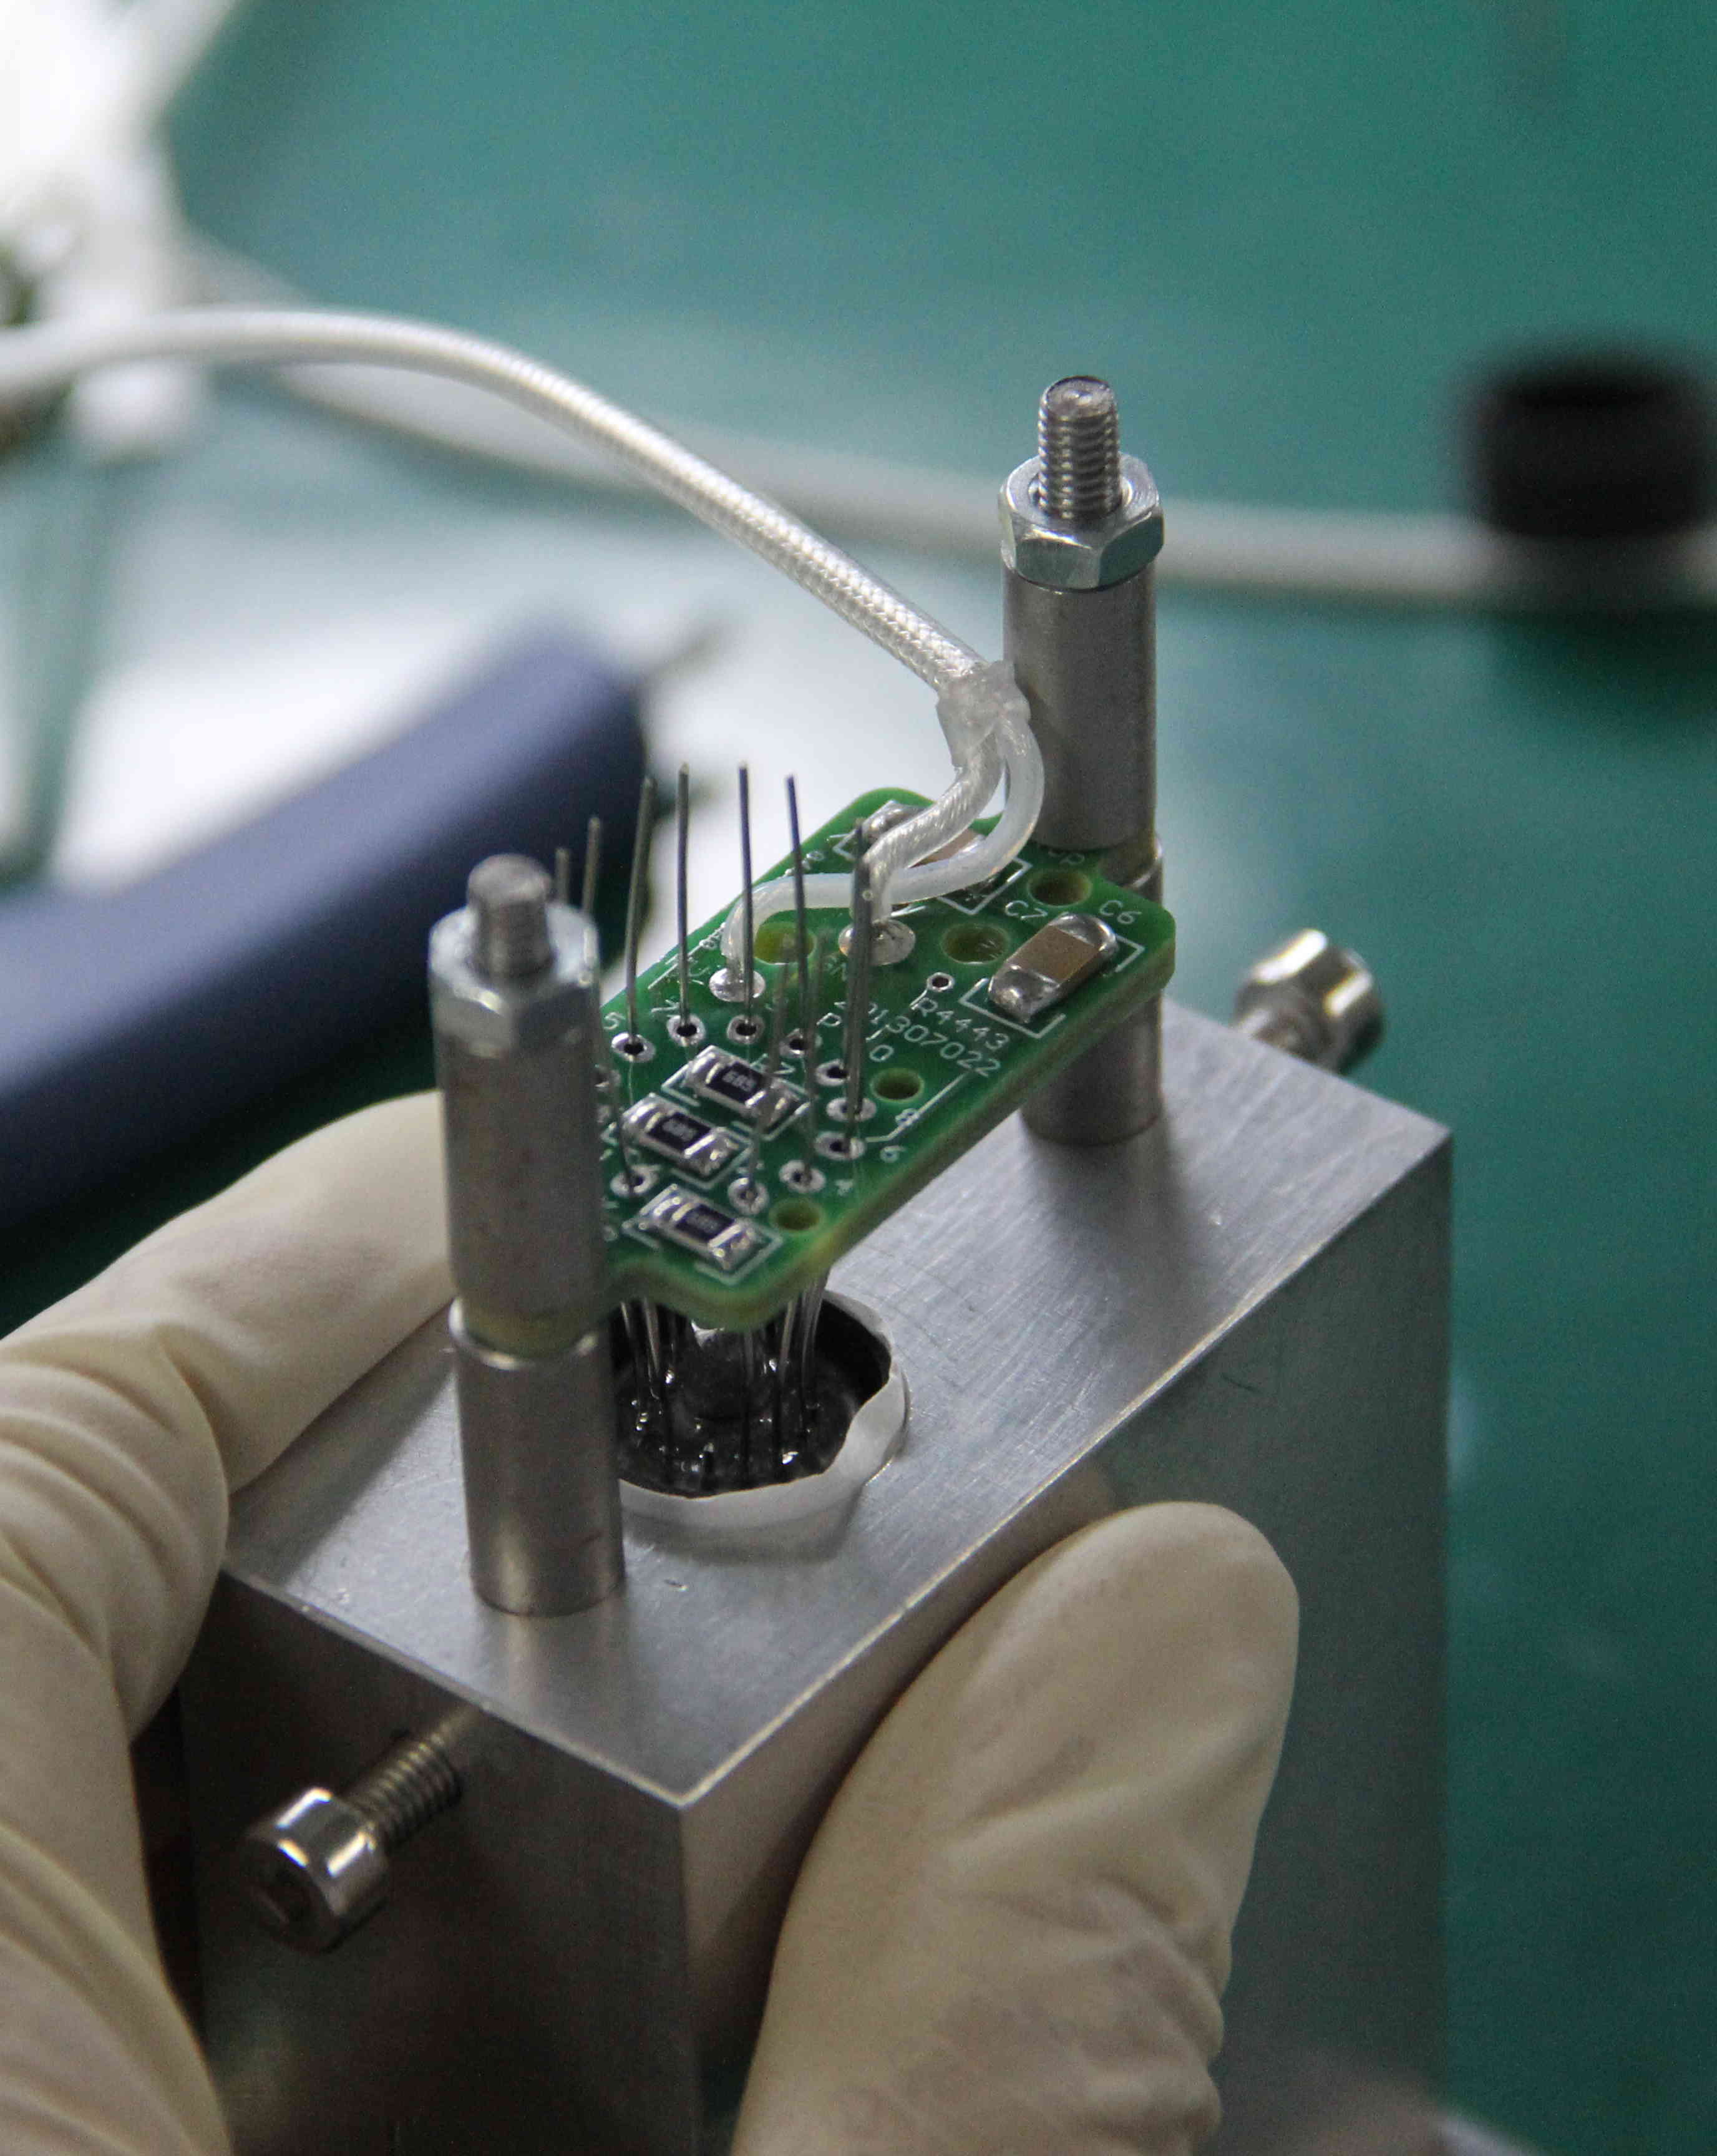
\includegraphics[width=0.32\textwidth]{chap/construction/fig/soldering_a.jpg}
}
% \hfill
\subfloat[][焊接第二块Base板]{
	\label{fig:construction:soldering_b}
	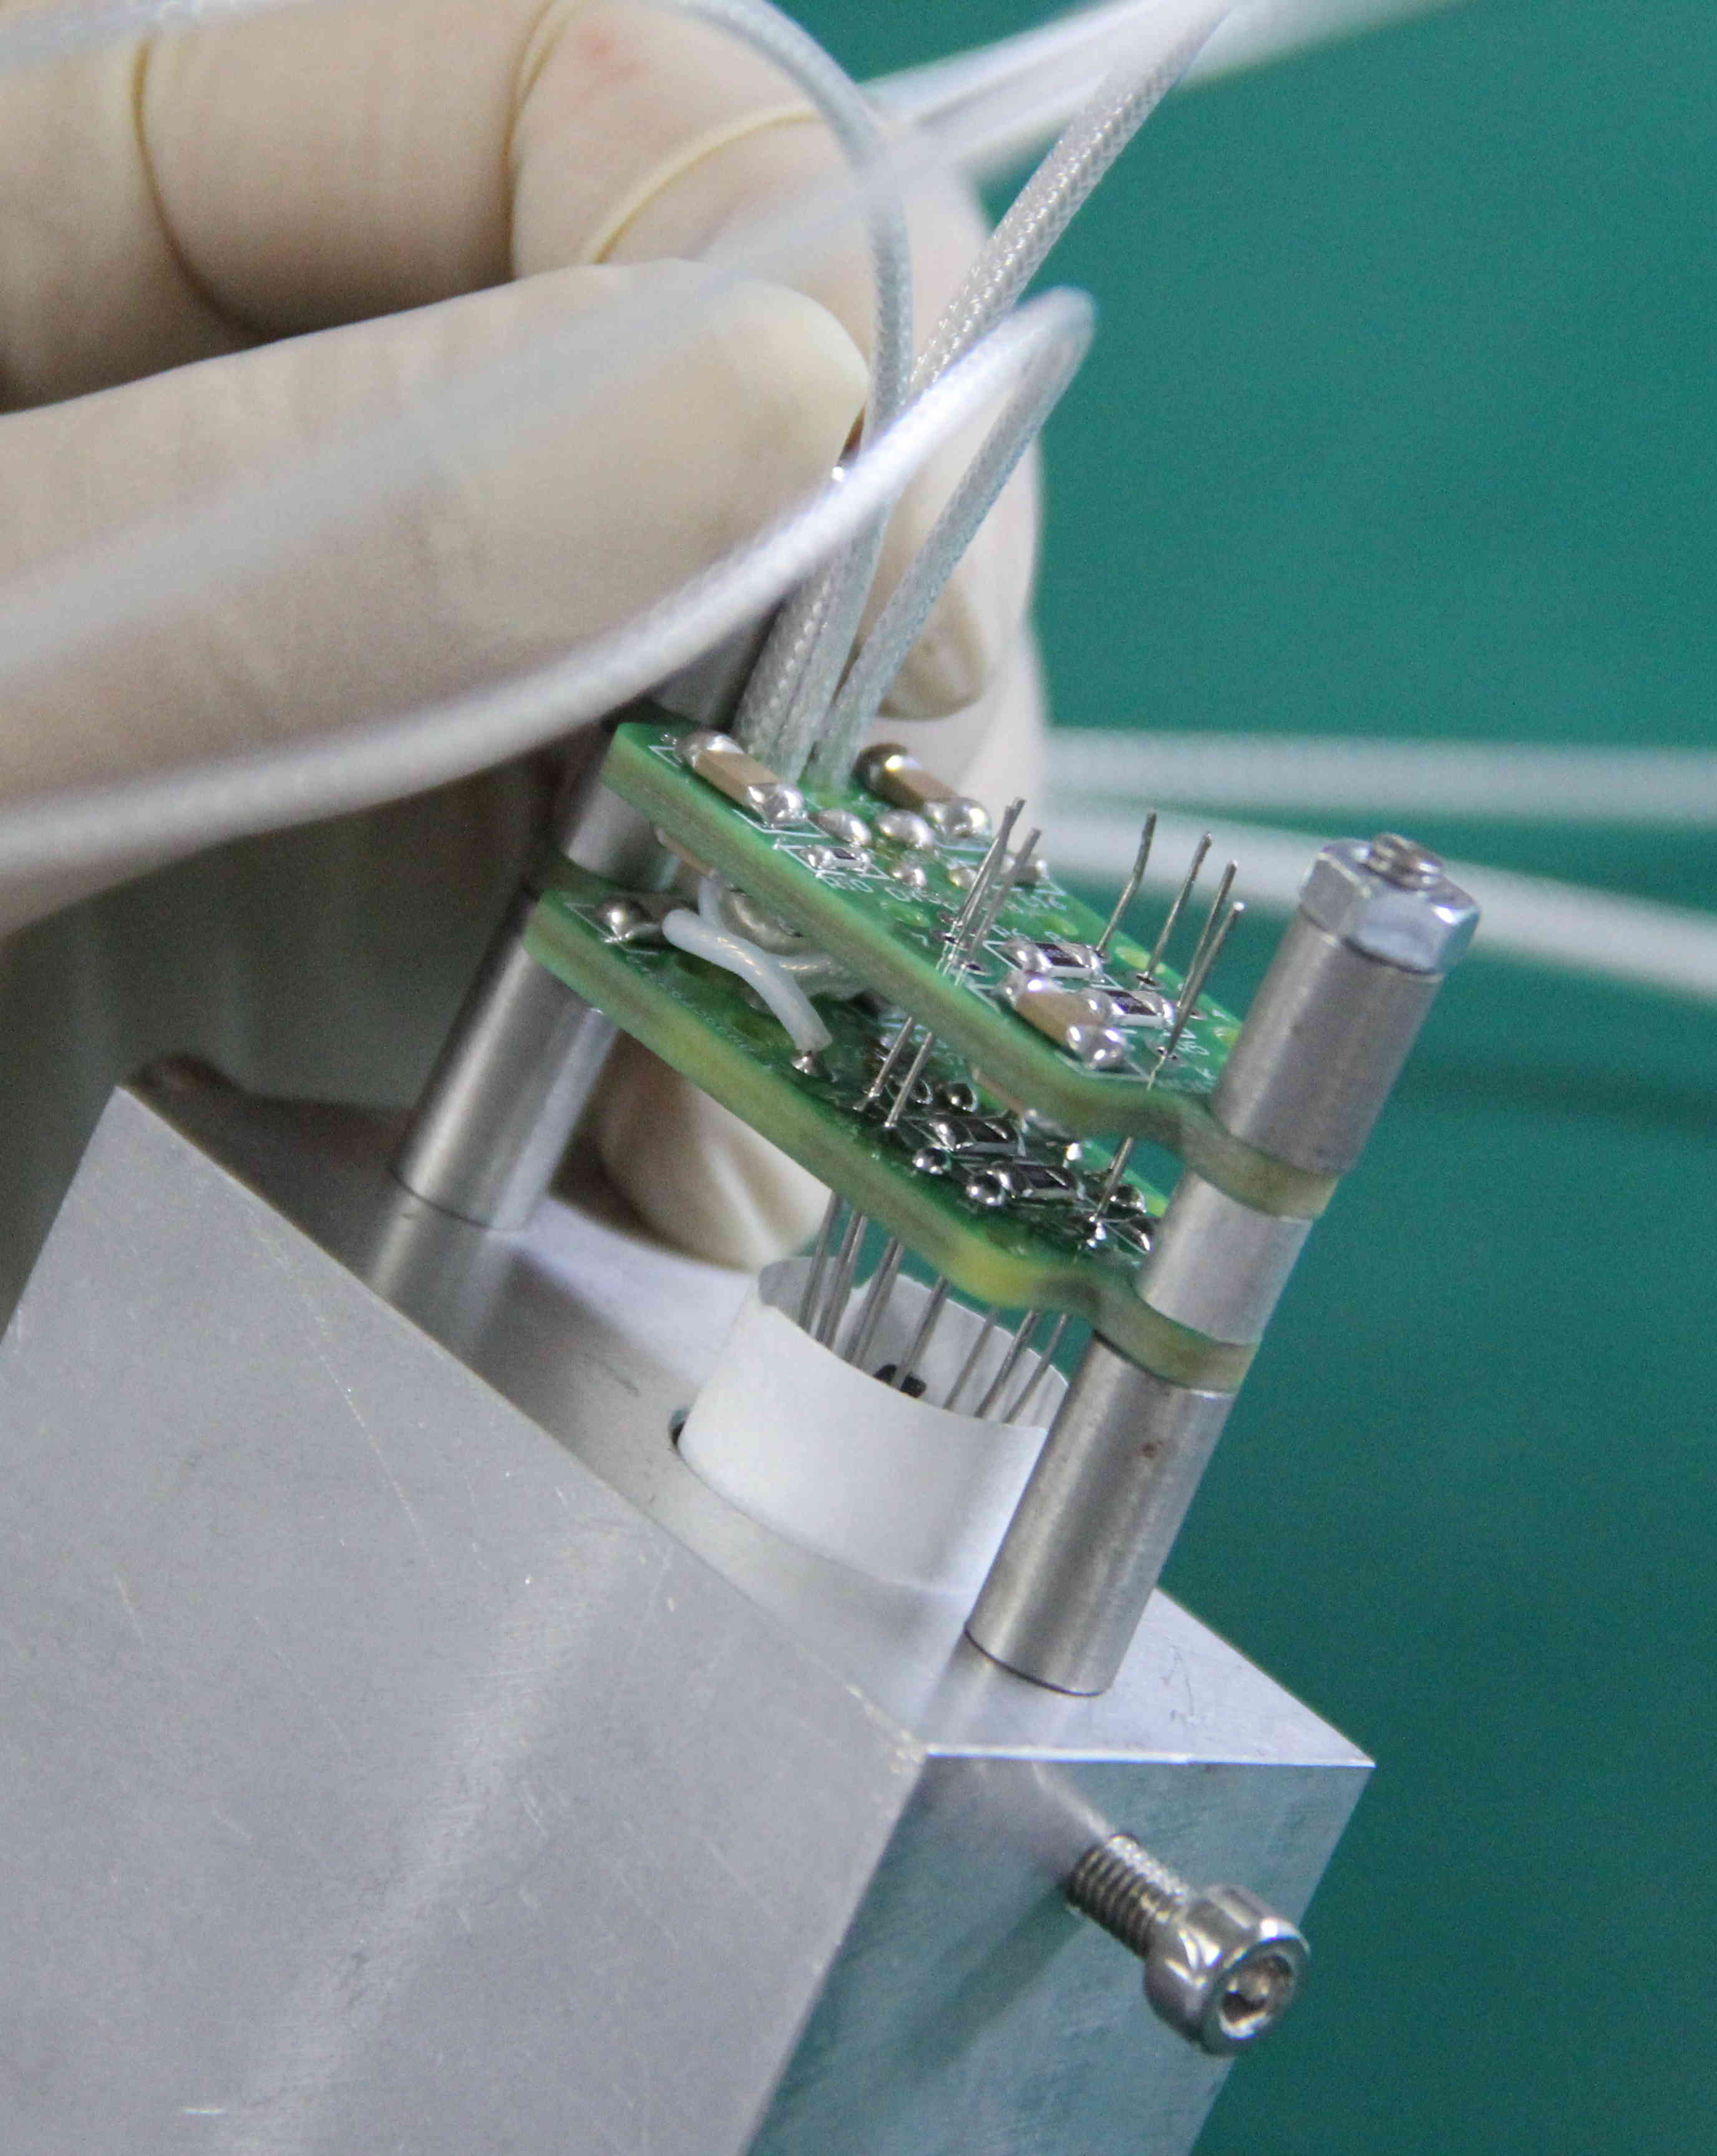
\includegraphics[width=0.32\textwidth]{chap/construction/fig/soldering_b.jpg}
}
% \subfloat[][焊接完成]{
% 	\label{fig:construction:soldering_c}
% 	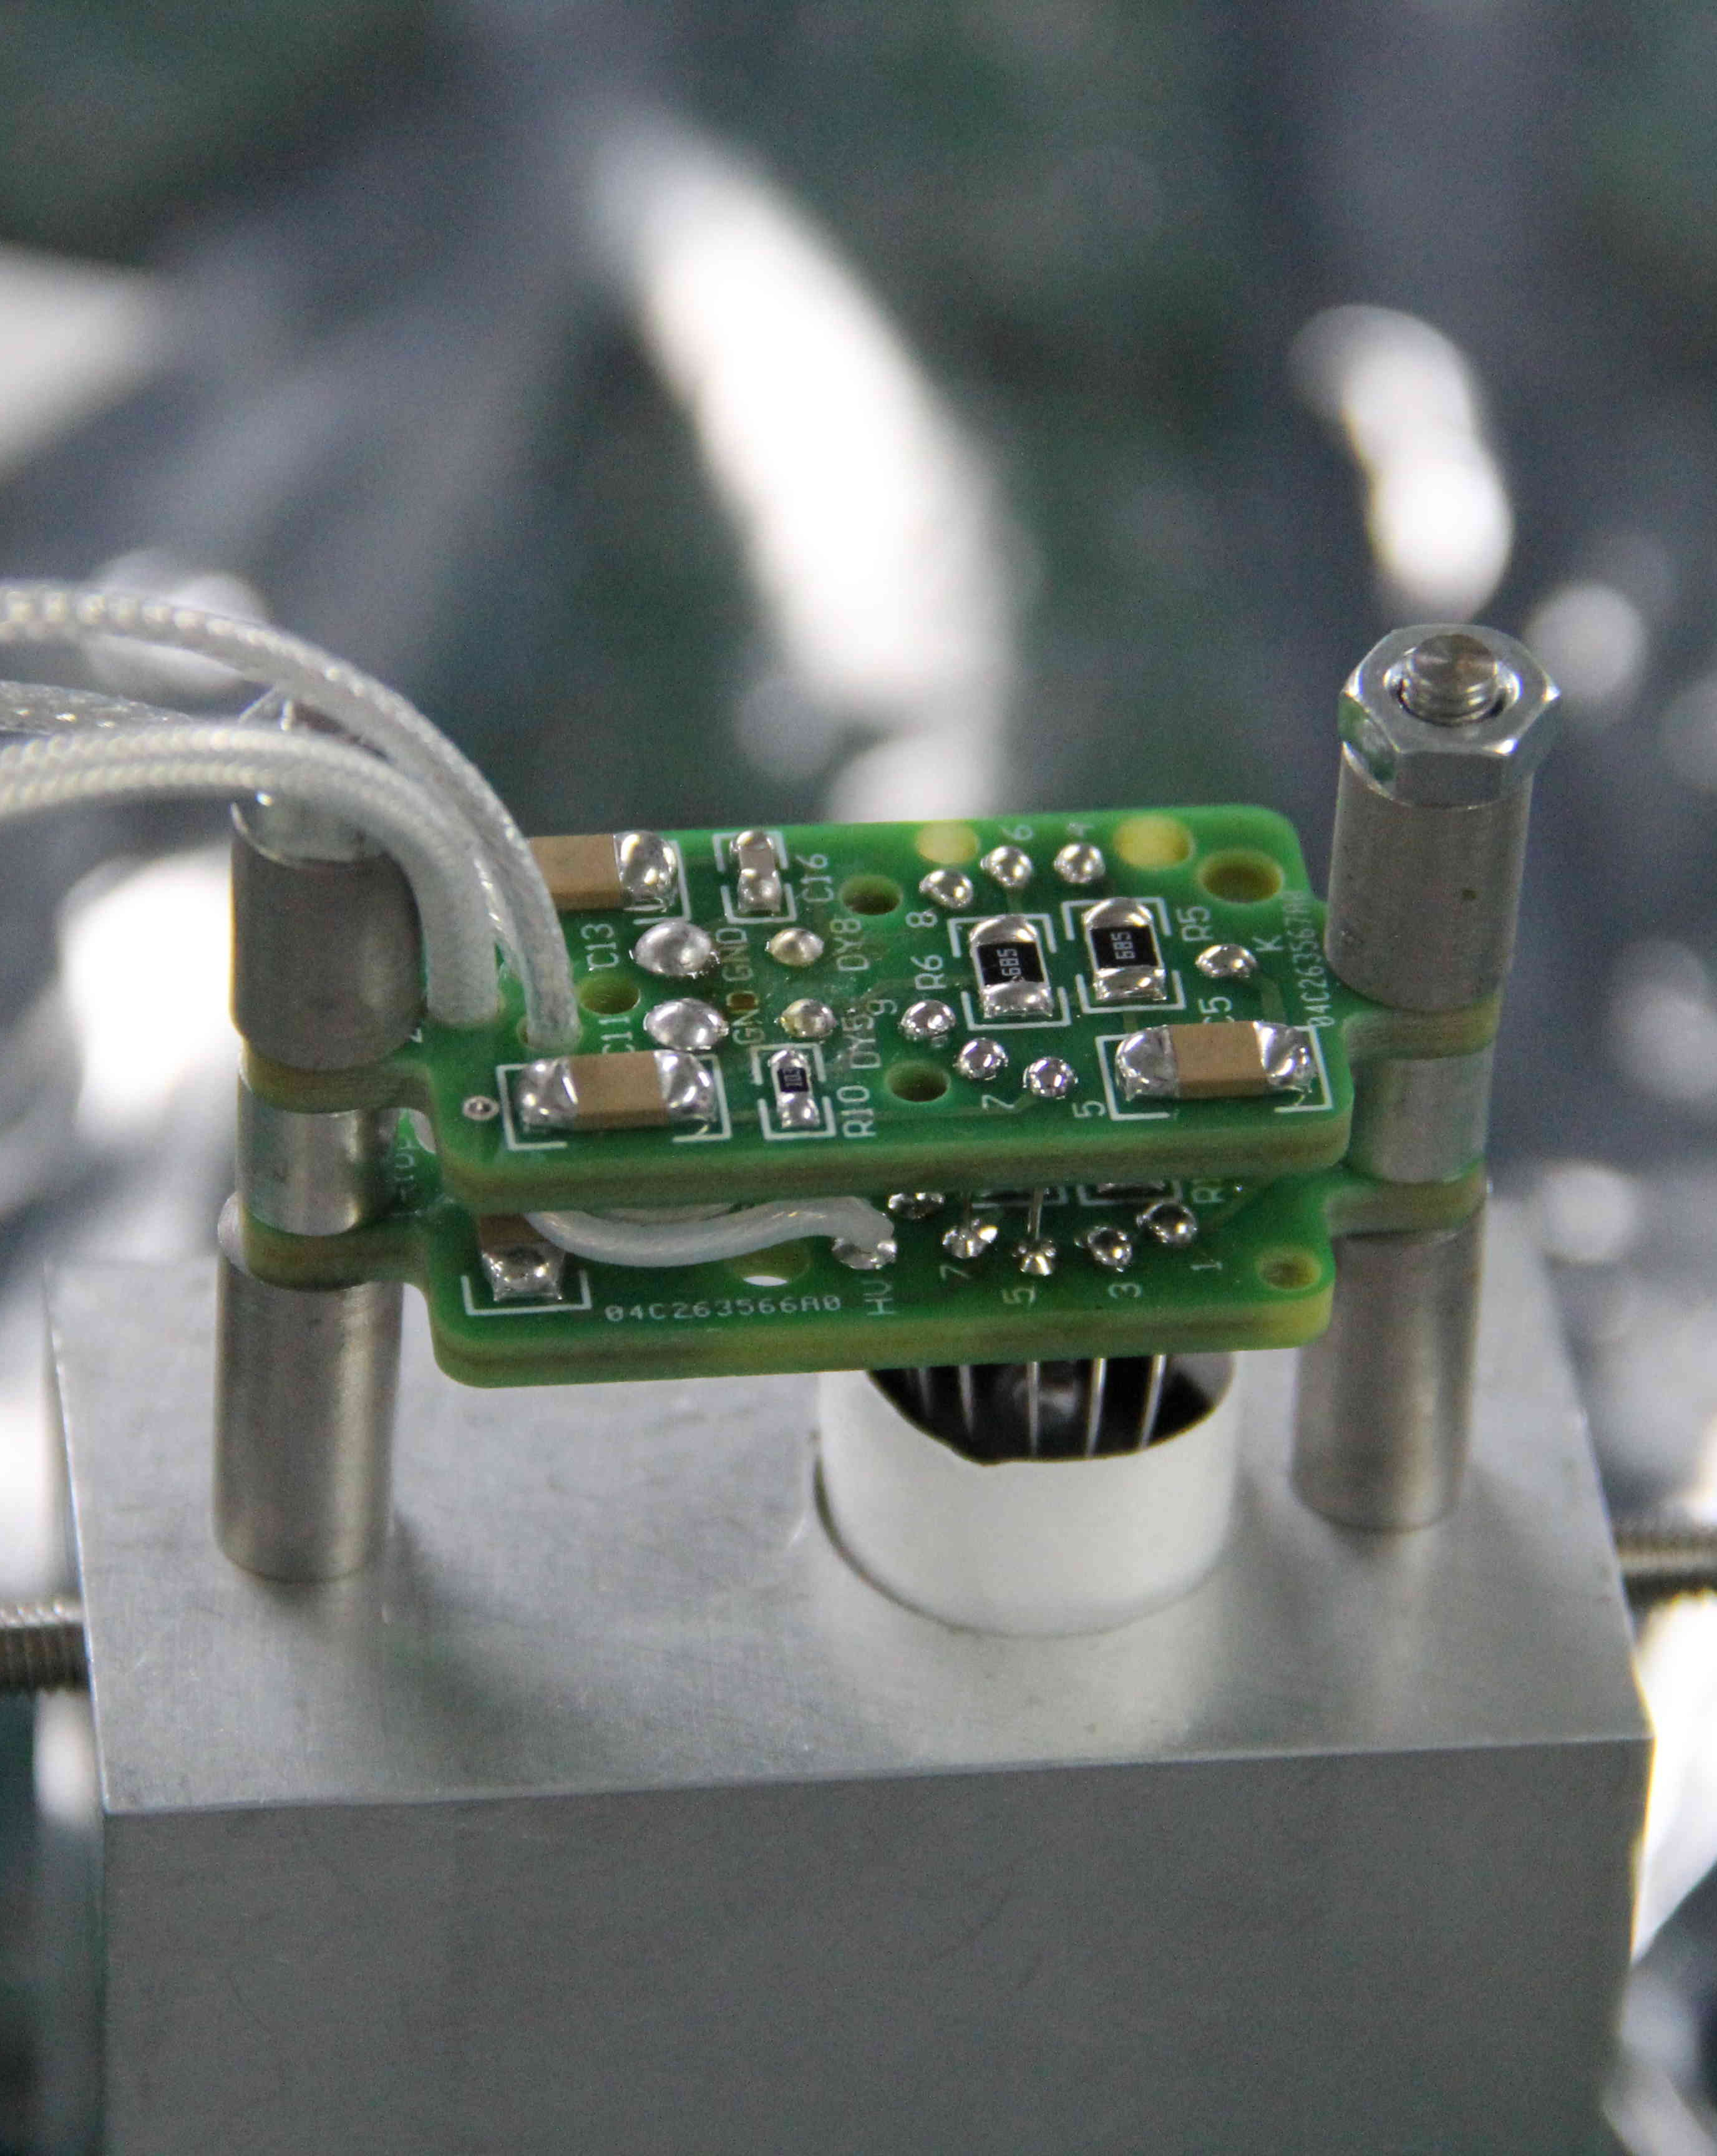
\includegraphics[width=0.24\textwidth]{chap/construction/fig/soldering_c.jpg}
% }
\subfloat[][对焊点进行清洗]{
	\label{fig:construction:soldering_d}
	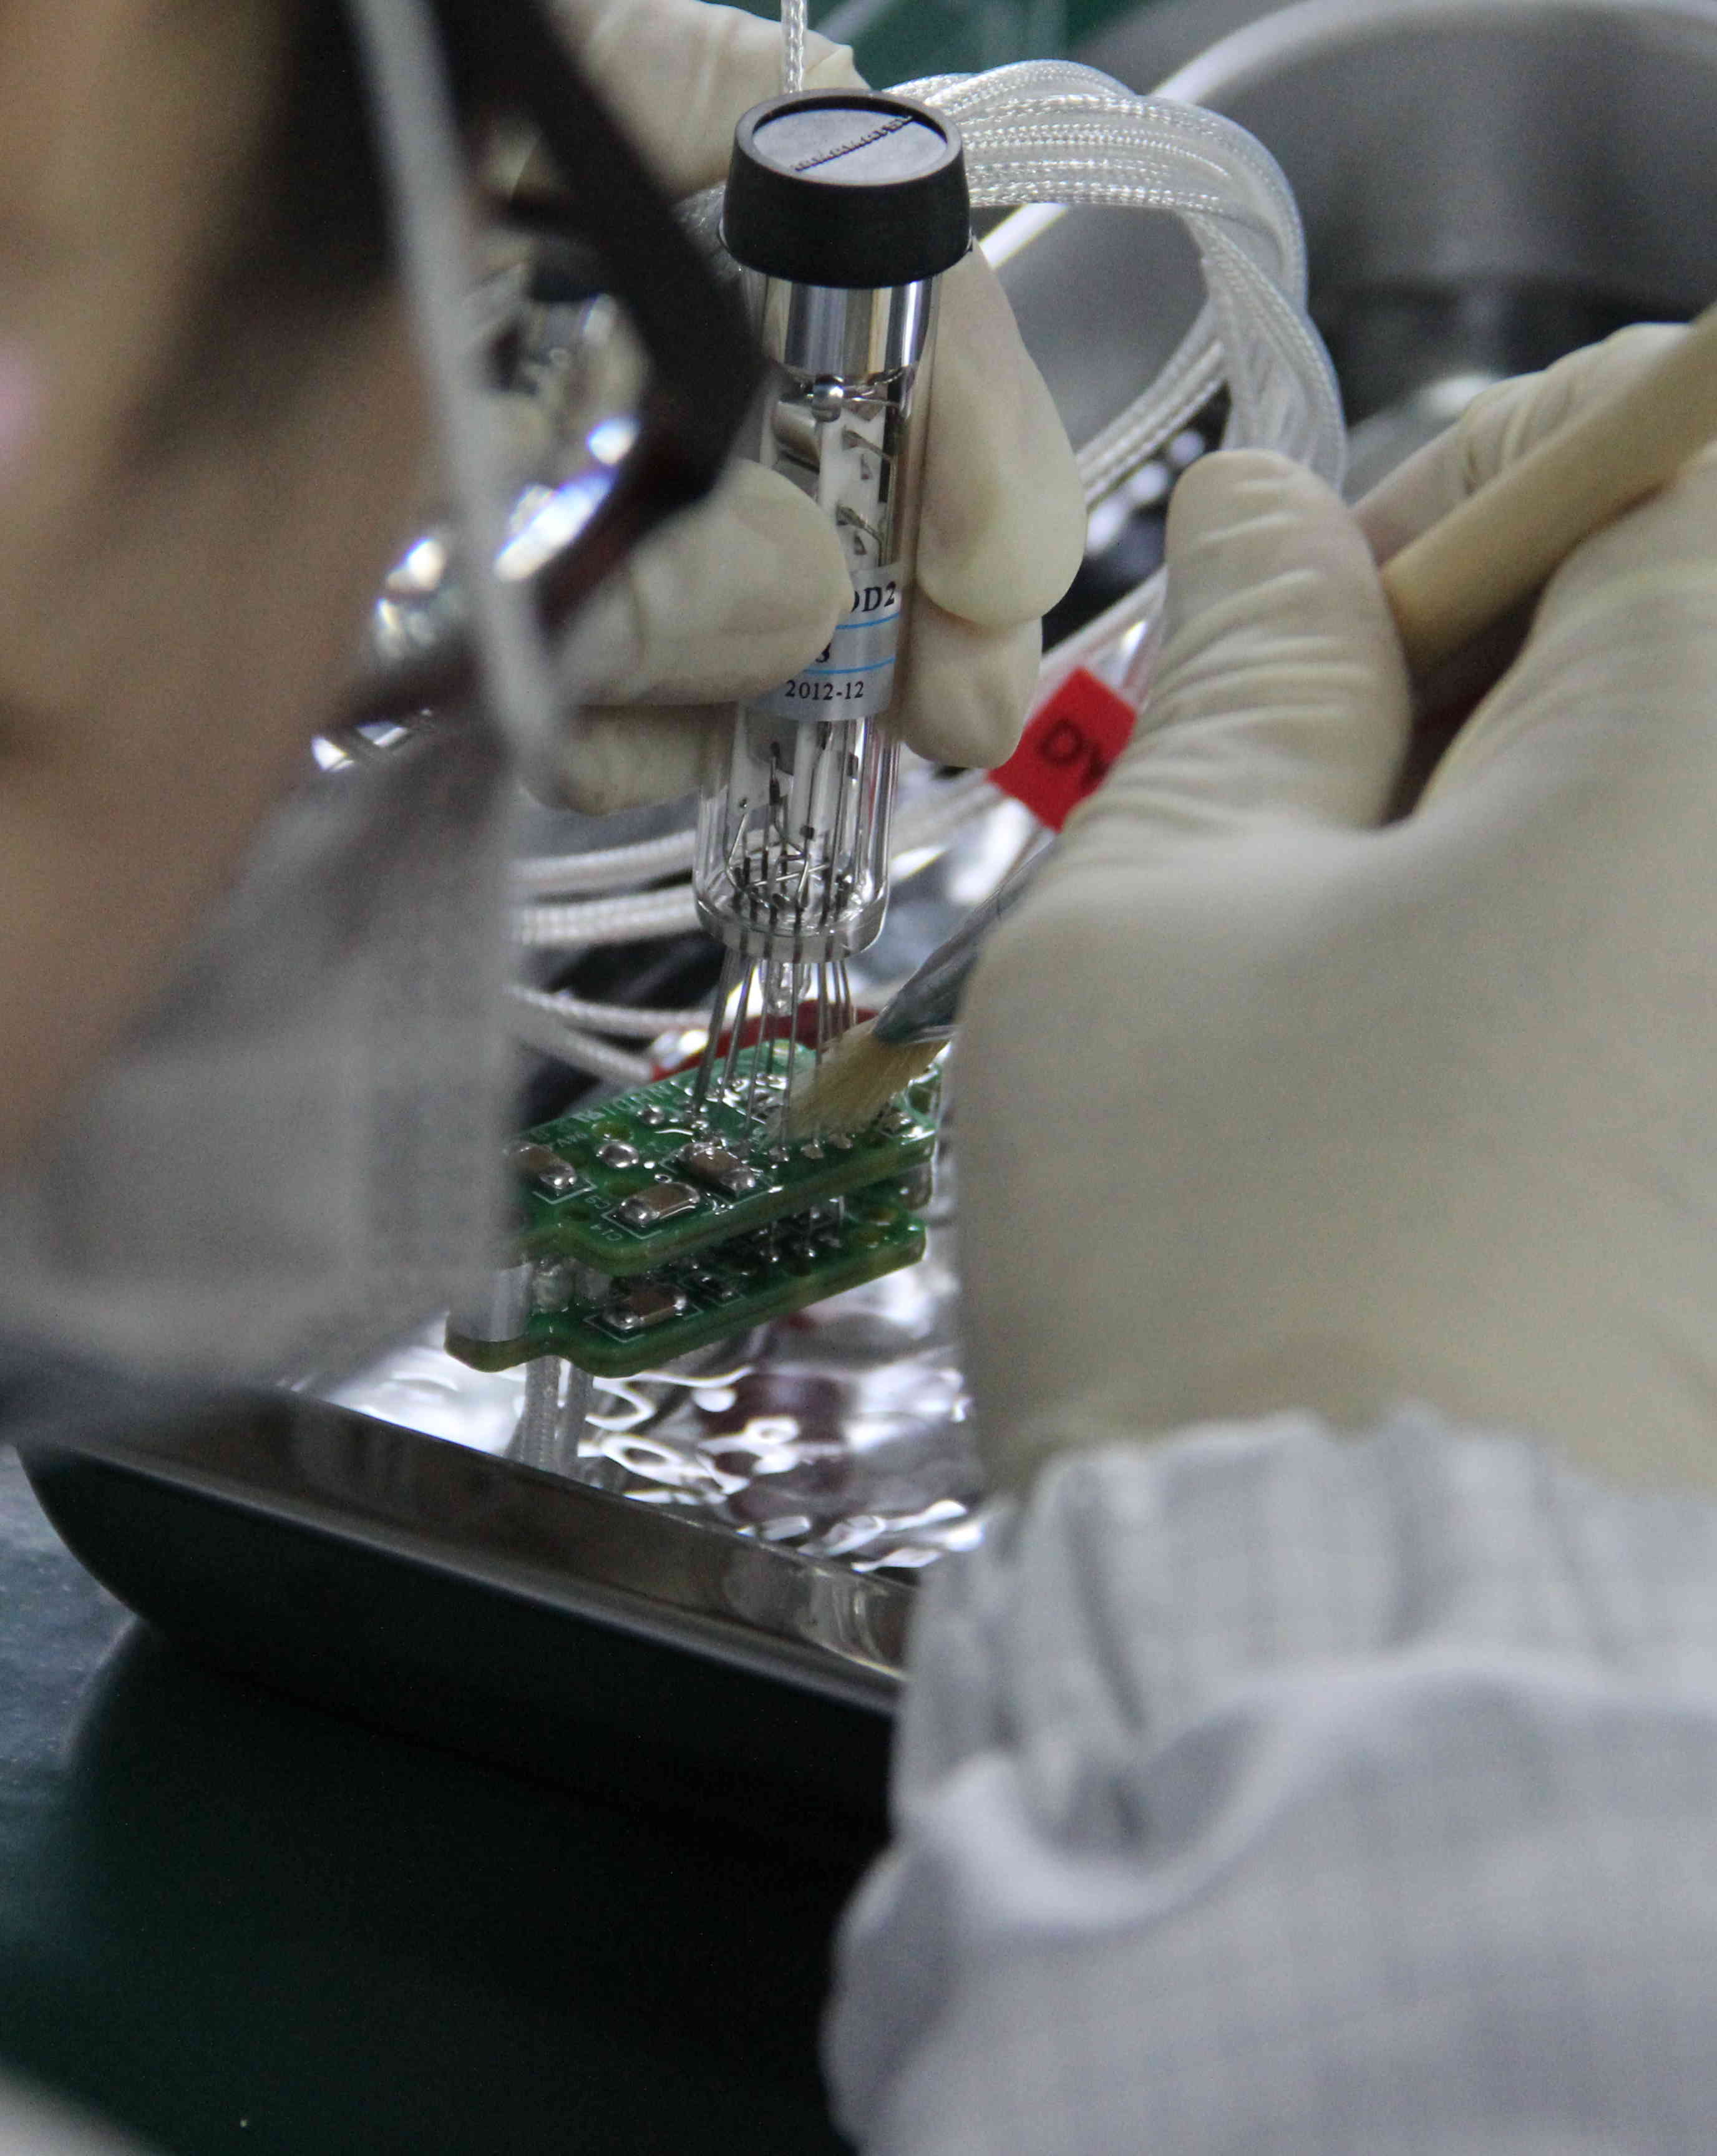
\includegraphics[width=0.32\textwidth]{chap/construction/fig/soldering_d.jpg}
}
\caption{R4443的Base电路板焊接流程}
\label{fig:construction:soldering}
\end{figure}
PMT组件灌封是PSD的关键生产步骤之一。为了解决硅橡胶的出气问题,保证灌封质量,一方面我们选取了能在恶劣空间环境下使用、出气率很低的双组分RTV胶作为灌封胶体;另一方面,我们制定了一系列控制措施以保证灌封操作的质量,如灌封前先将胶体放在真空靶室中抽气、设计专门的透明工装以便于观察气泡等等。
具体的灌封步骤如图\ref{fig:construction:potting}所示,其中需要特别说明的是:我们在安装完硅脂垫片后,在R4443端头耦合面附近又缠绕了几圈Teflon(见图\ref{fig:construction:potting_a}),以防止胶体渗入R4443与硅脂垫片的耦合面,导致影响输入光强度。
\begin{figure}[htb]
\centering
\subfloat[][安装硅脂垫片]{
	\label{fig:construction:potting_a}
	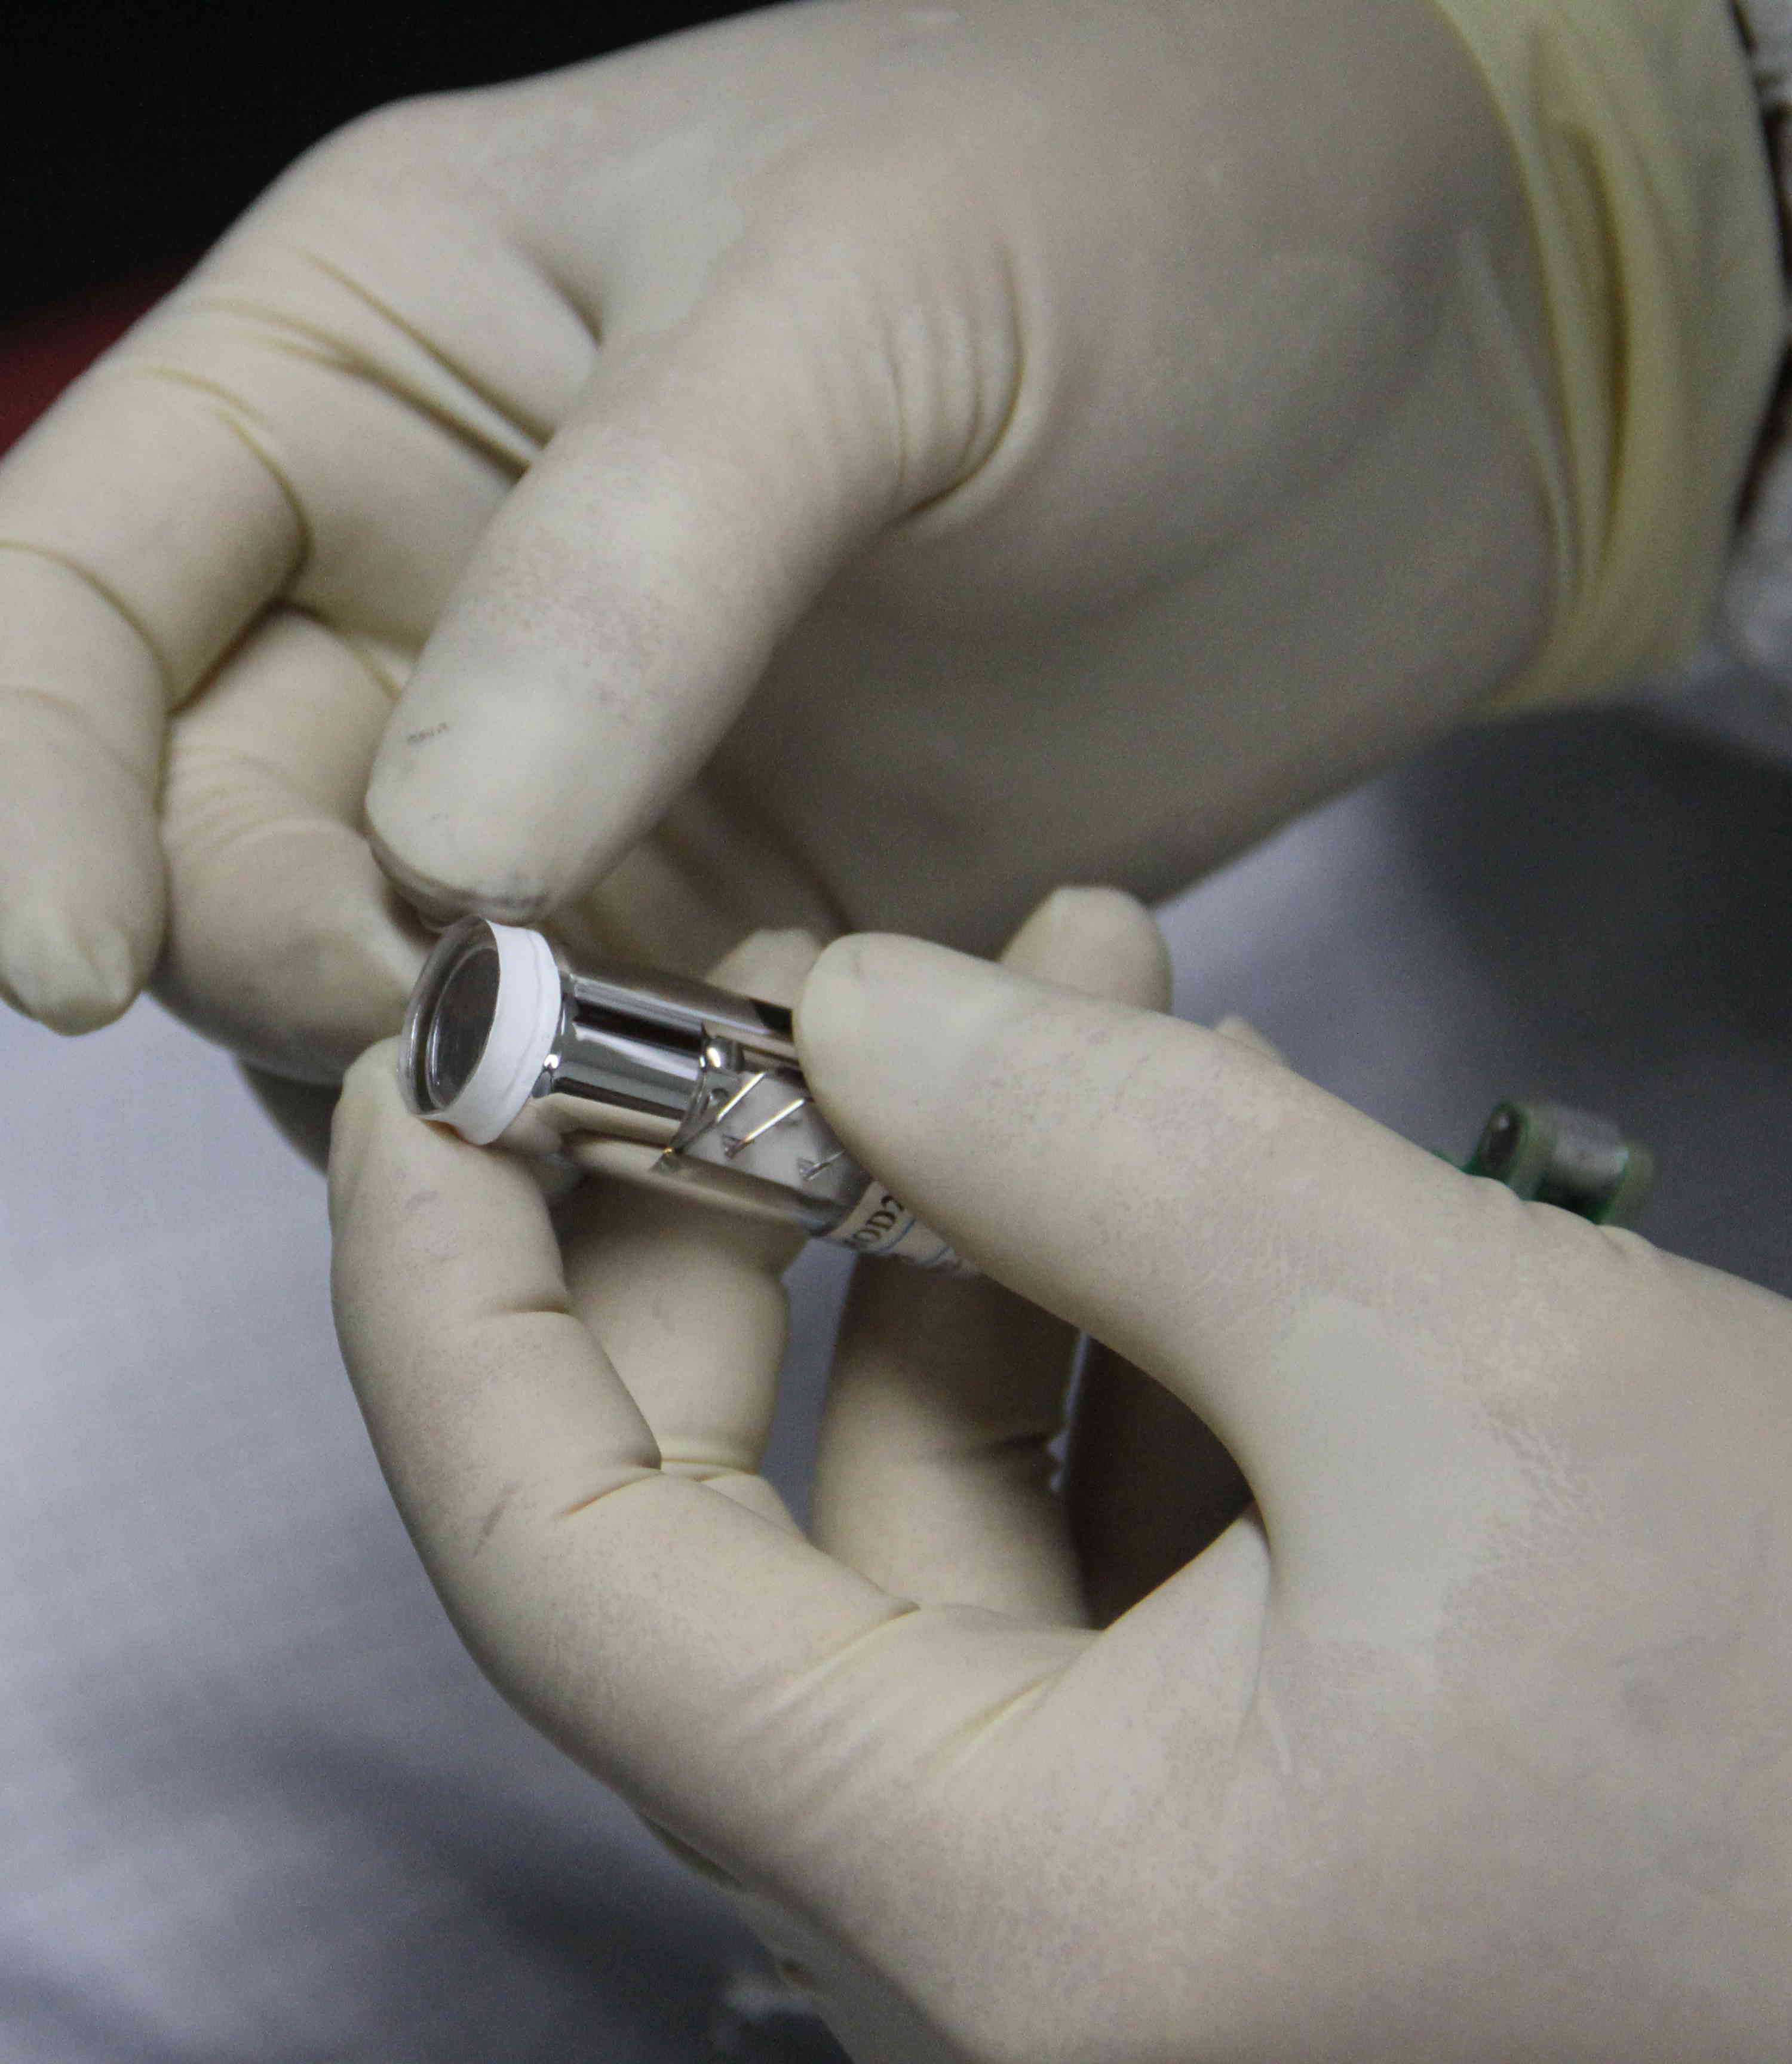
\includegraphics[width=0.32\textwidth]{chap/construction/fig/potting_a.jpg}
}
\subfloat[][将PMT装入透明灌封工装中]{
	\label{fig:construction:potting_b}
	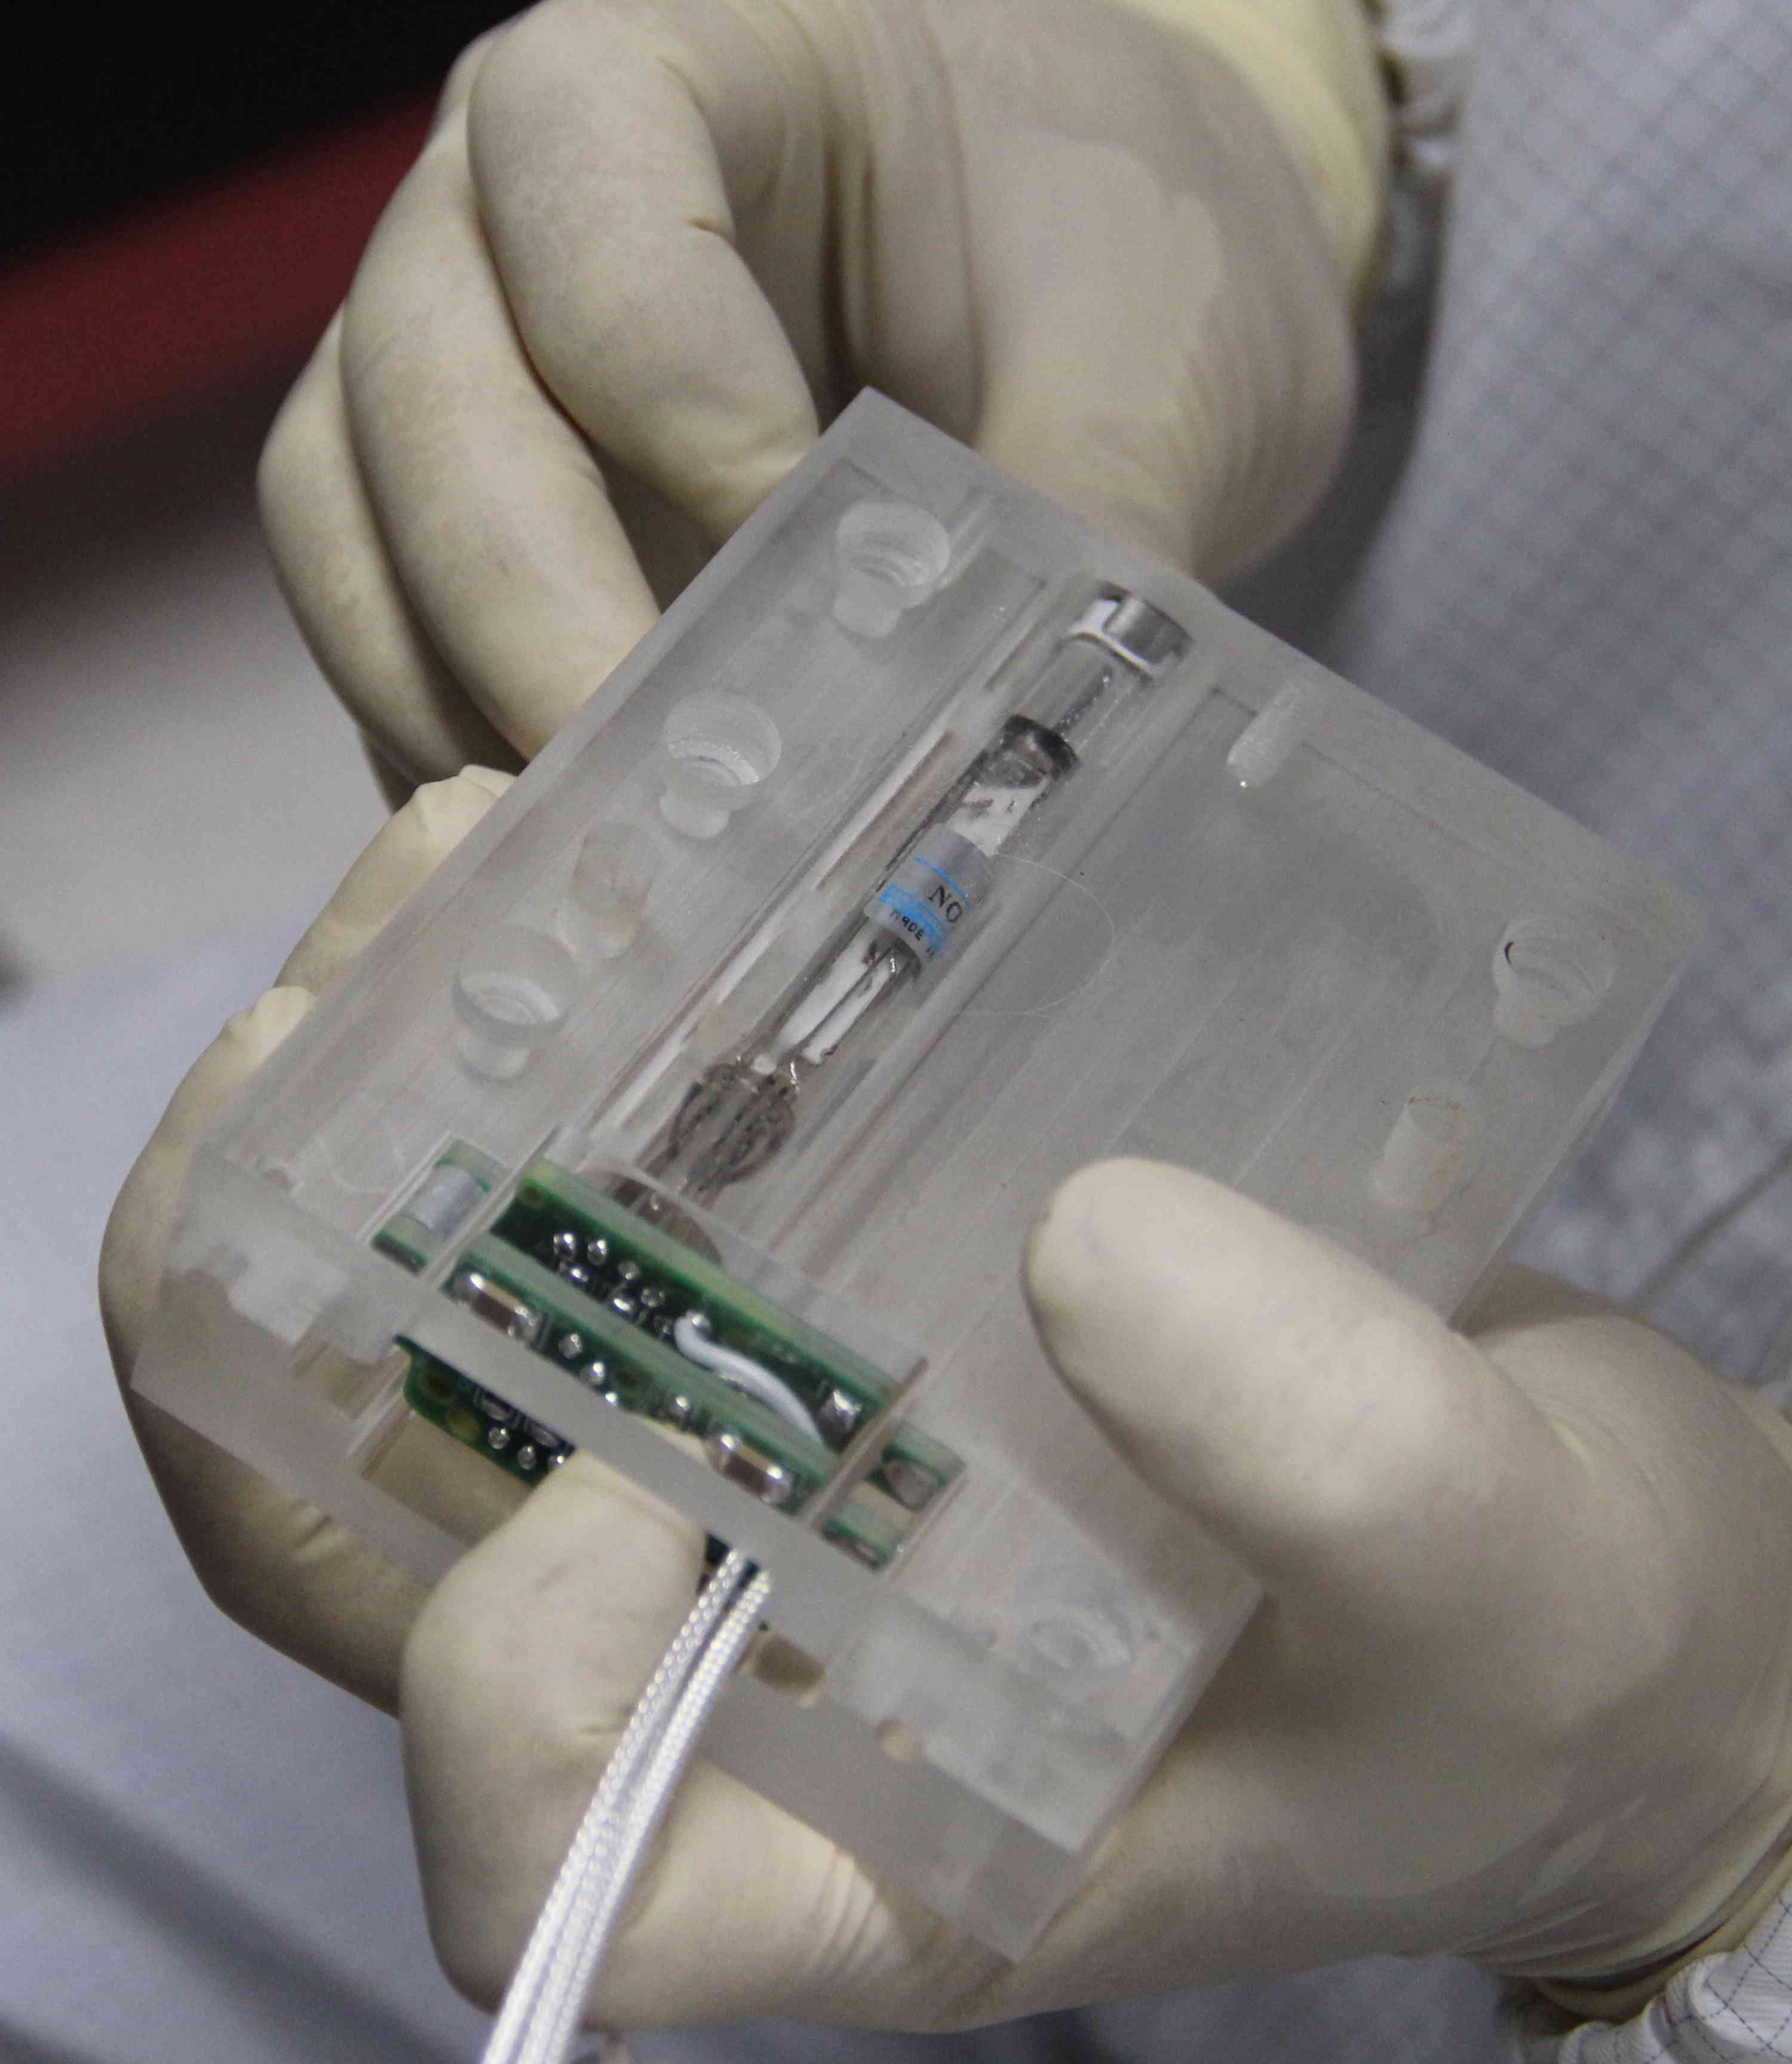
\includegraphics[width=0.32\textwidth]{chap/construction/fig/potting_b.jpg}
}
\subfloat[][灌封避光胶部分]{
	\label{fig:construction:potting_c}
	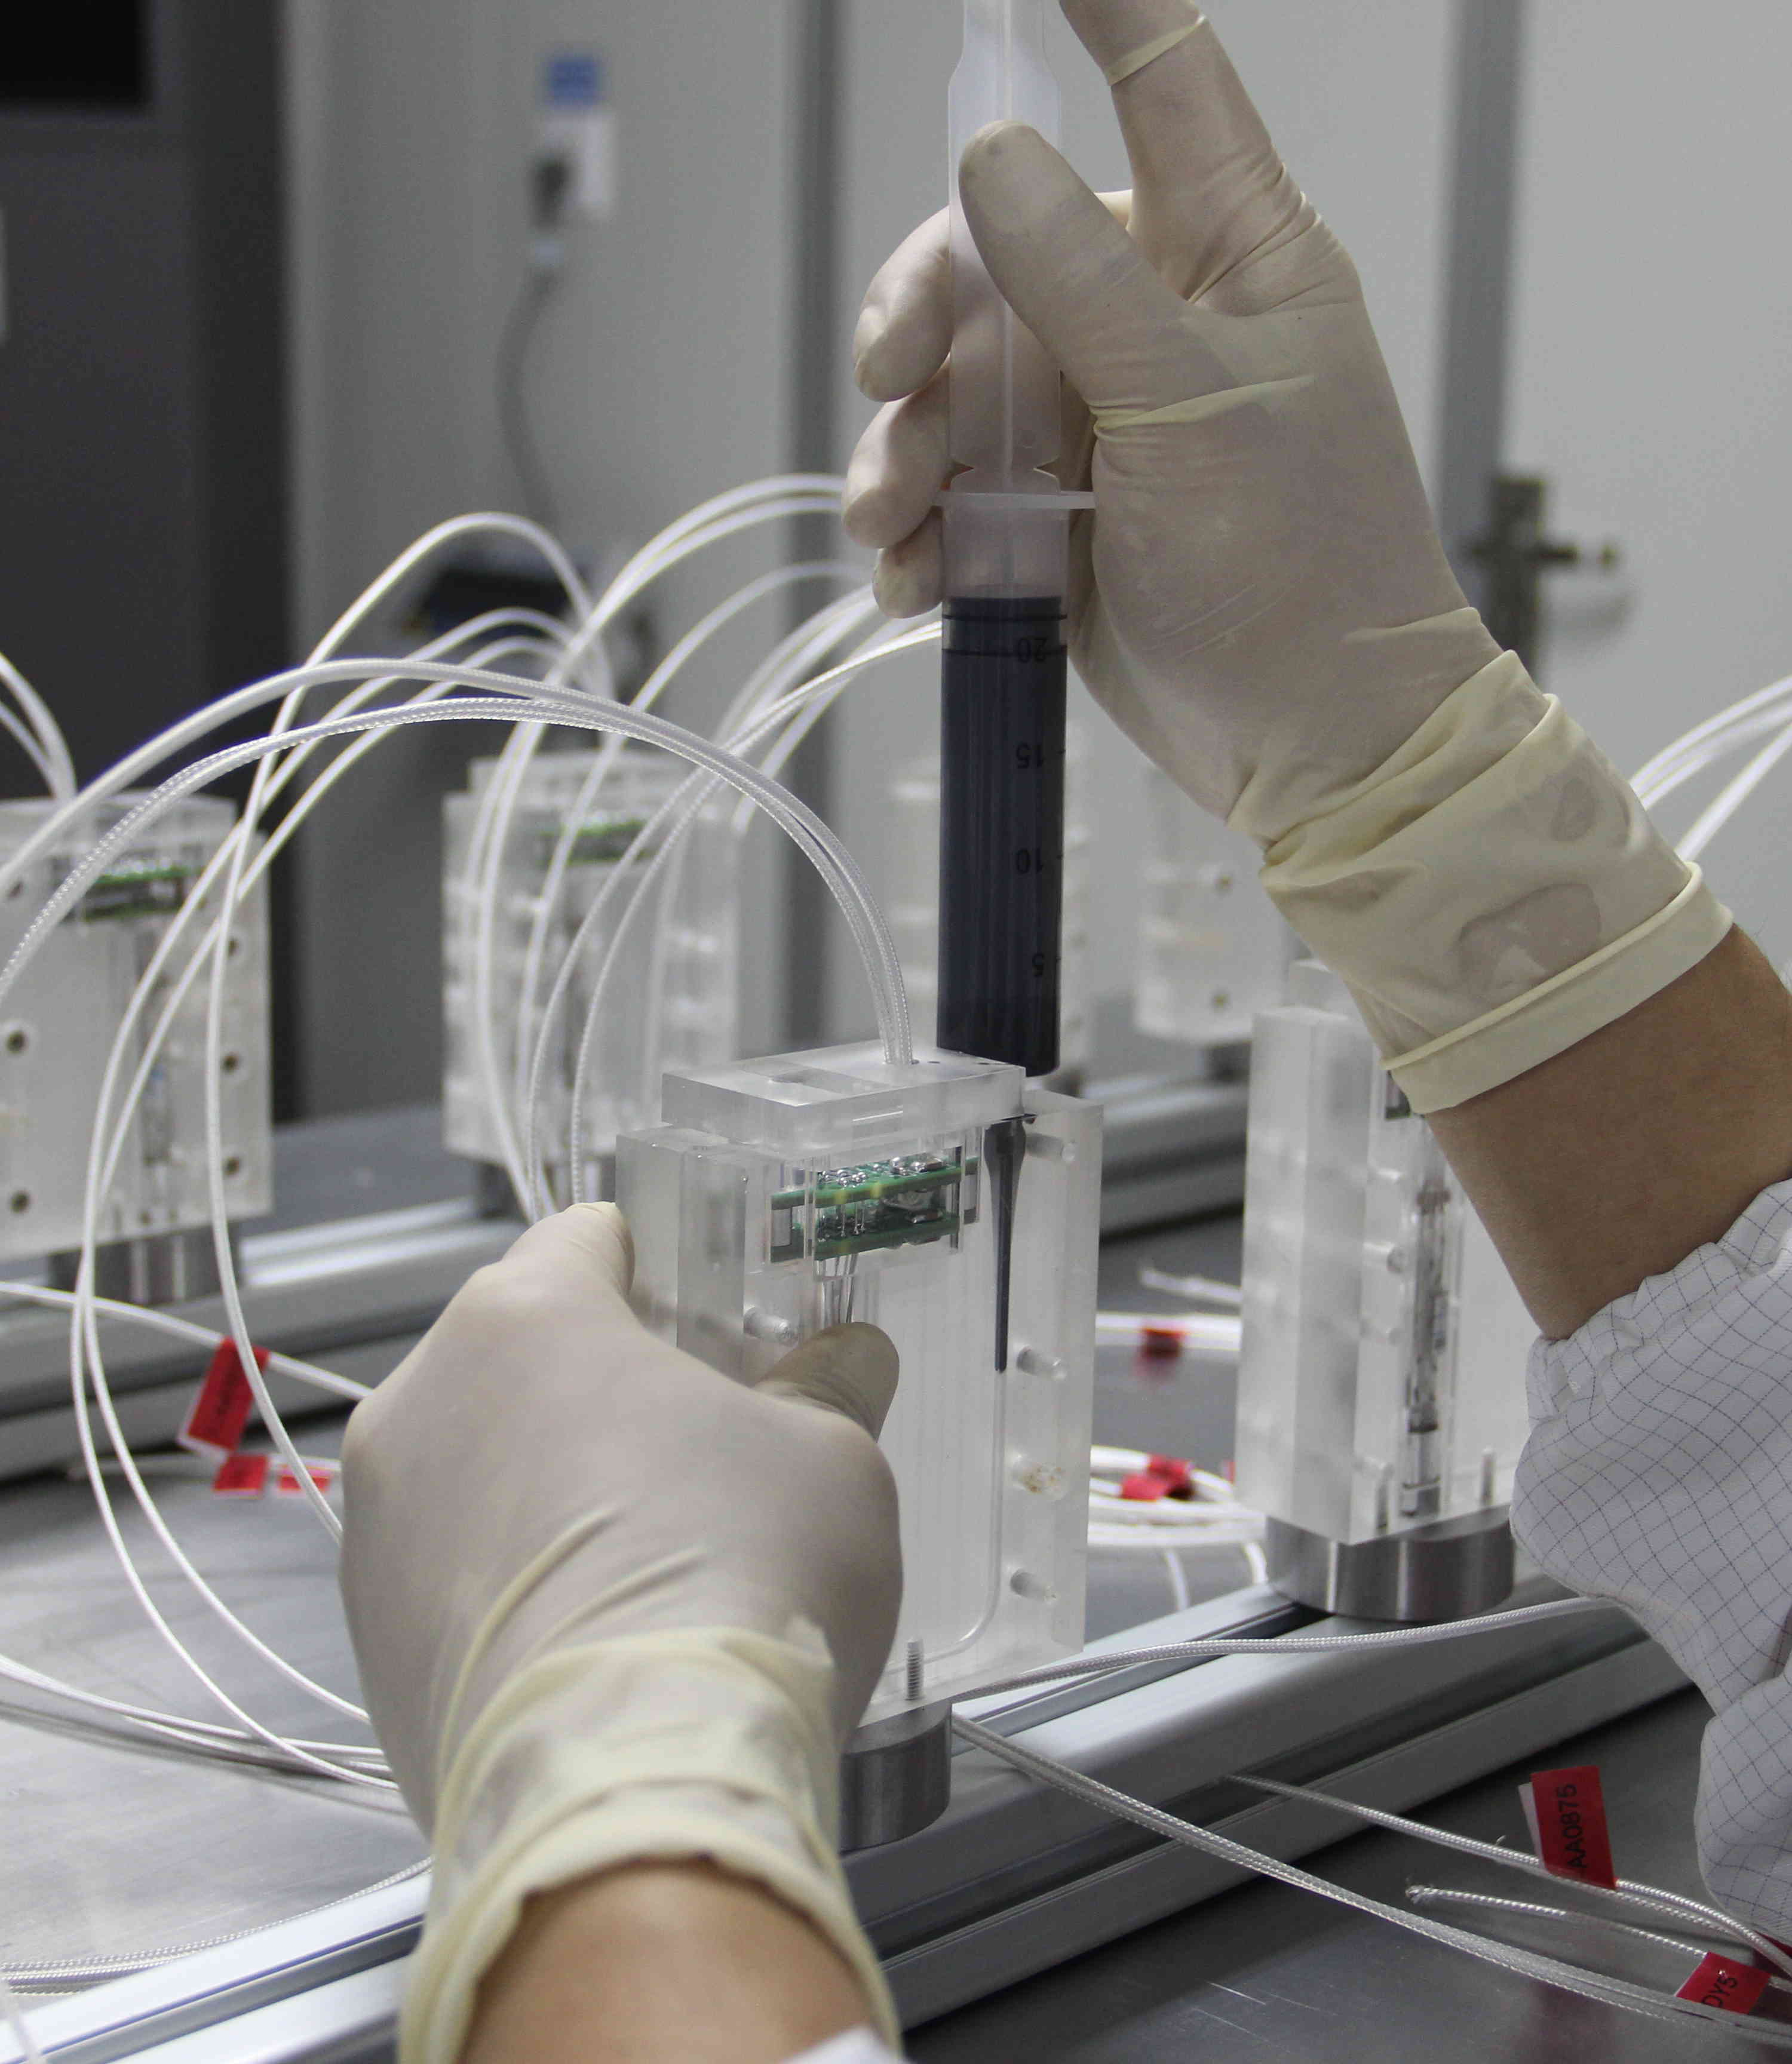
\includegraphics[width=0.32\textwidth]{chap/construction/fig/potting_c.jpg}
}
//
\subfloat[][灌封绝缘胶部分]{
	\label{fig:construction:potting_d}
	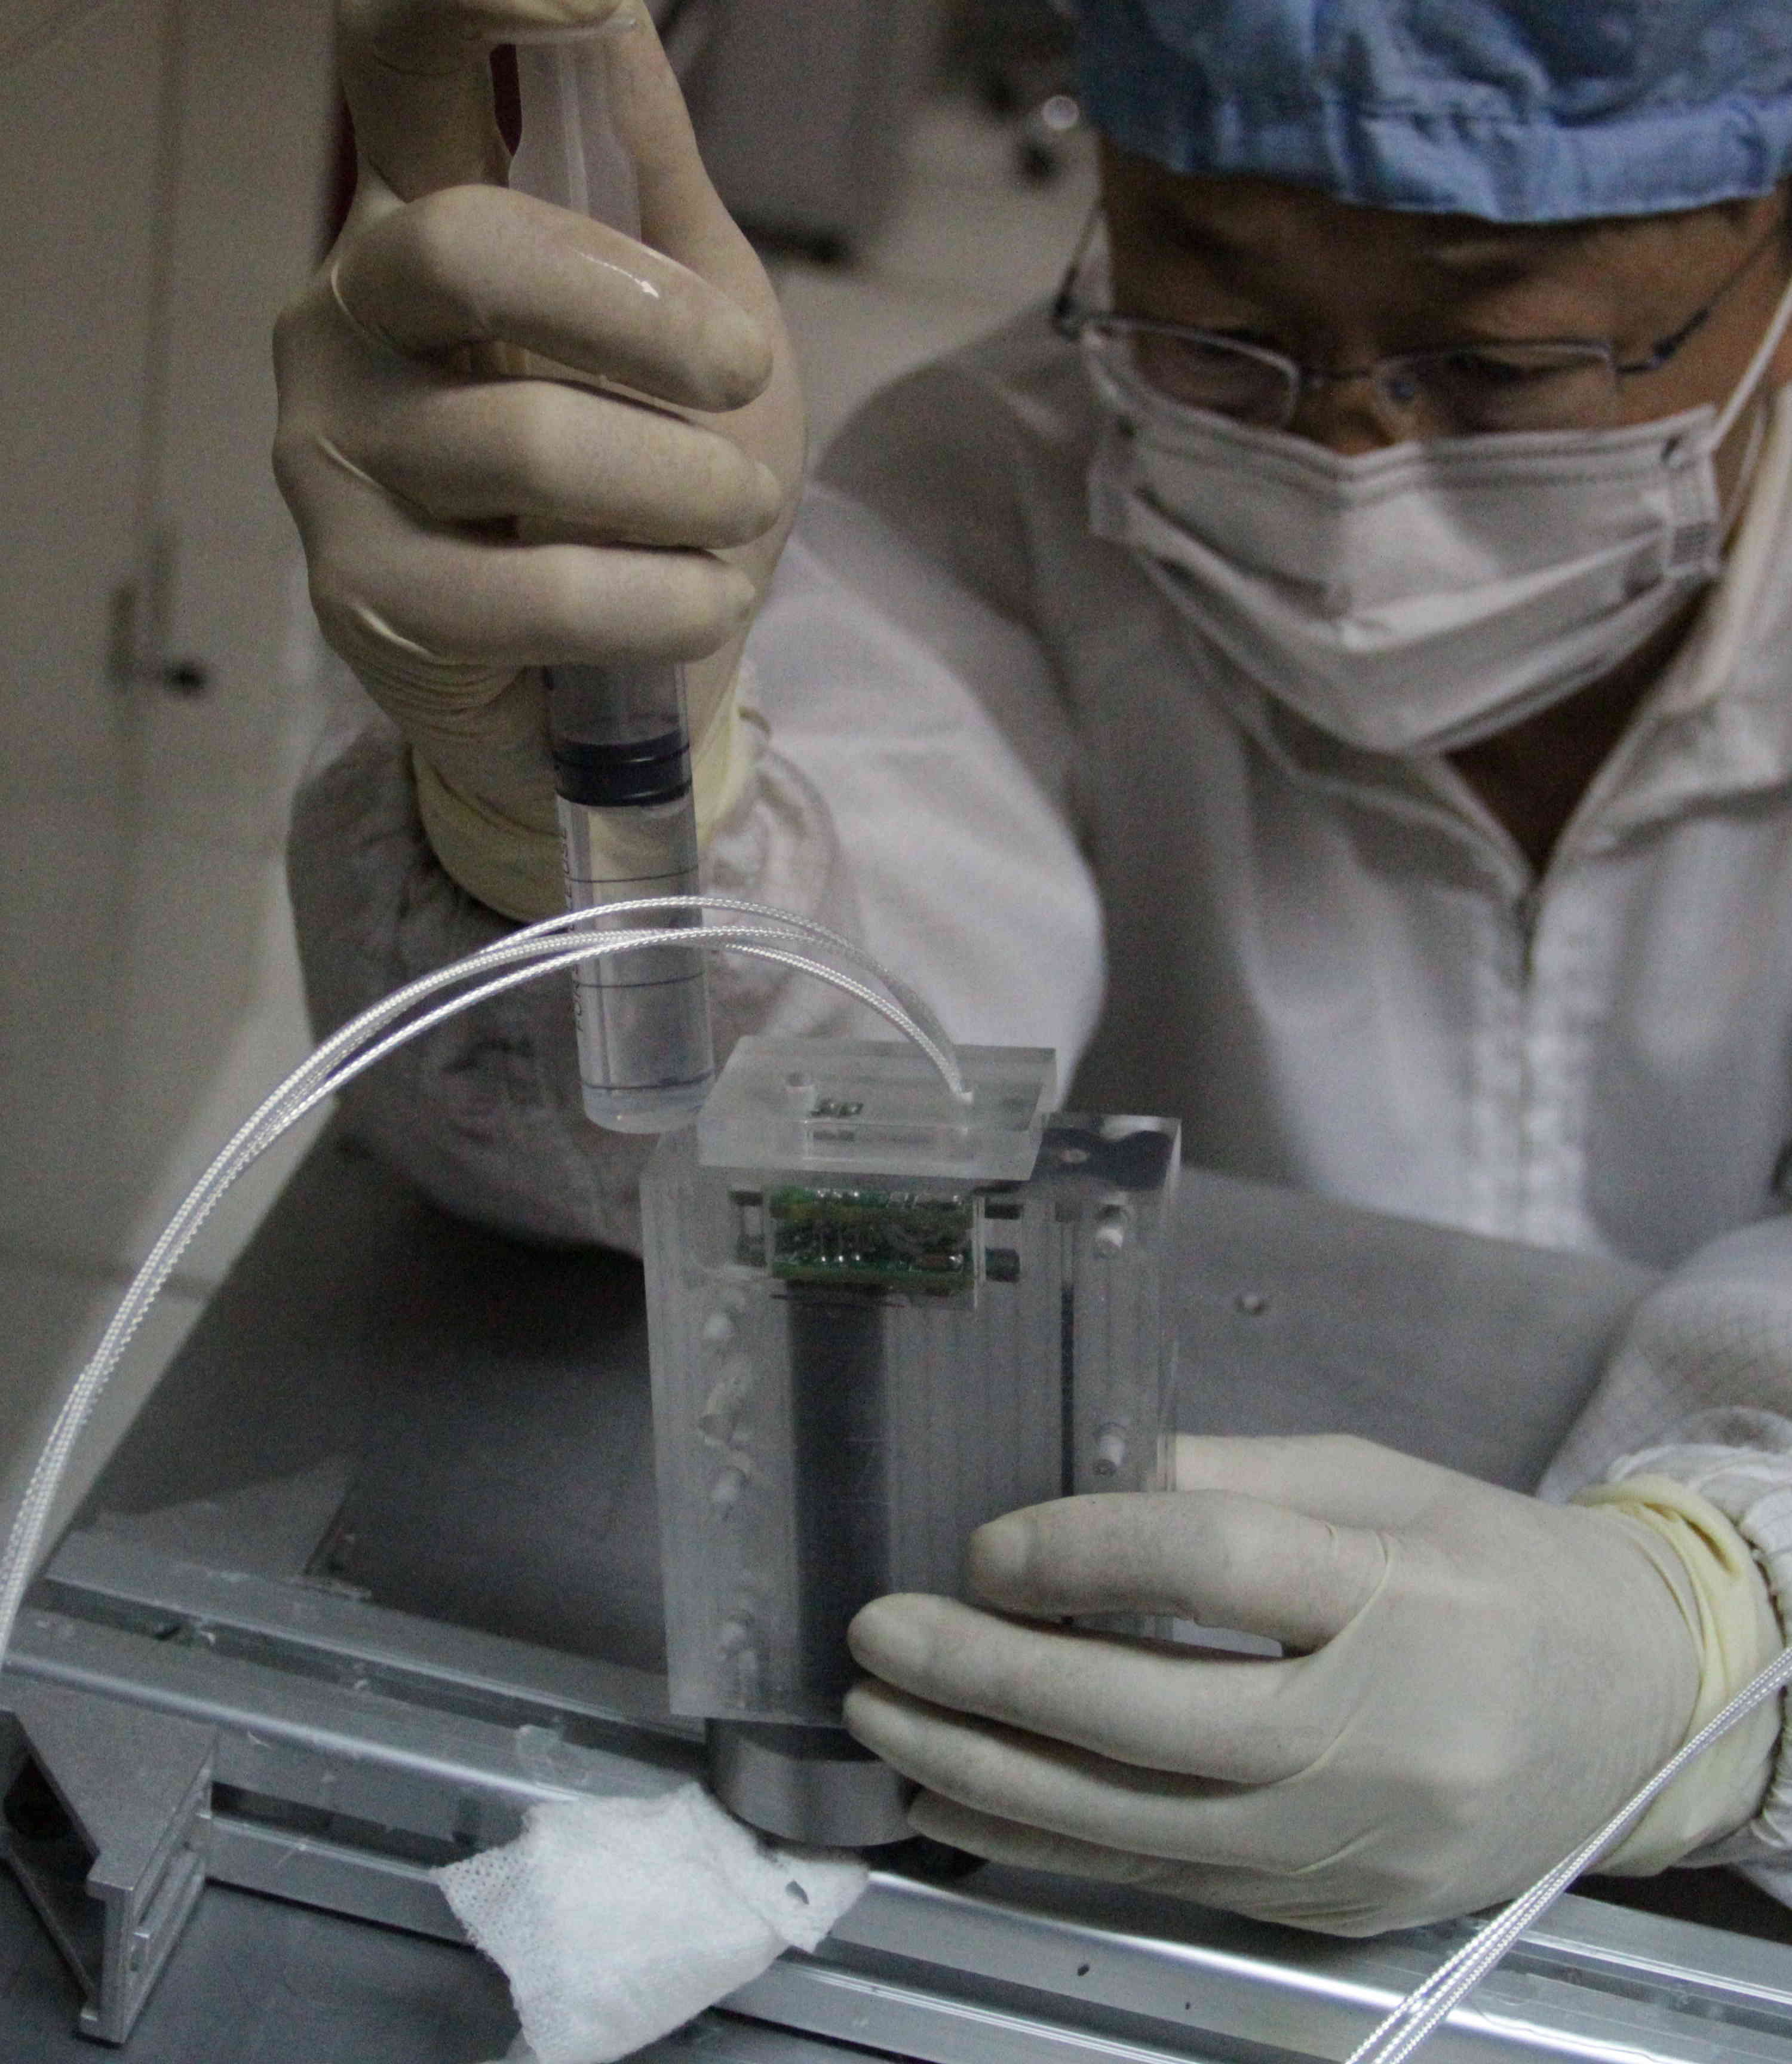
\includegraphics[width=0.32\textwidth]{chap/construction/fig/potting_d.jpg}
}
\subfloat[][静置,等待胶体凝固]{
	\label{fig:construction:potting_e}
	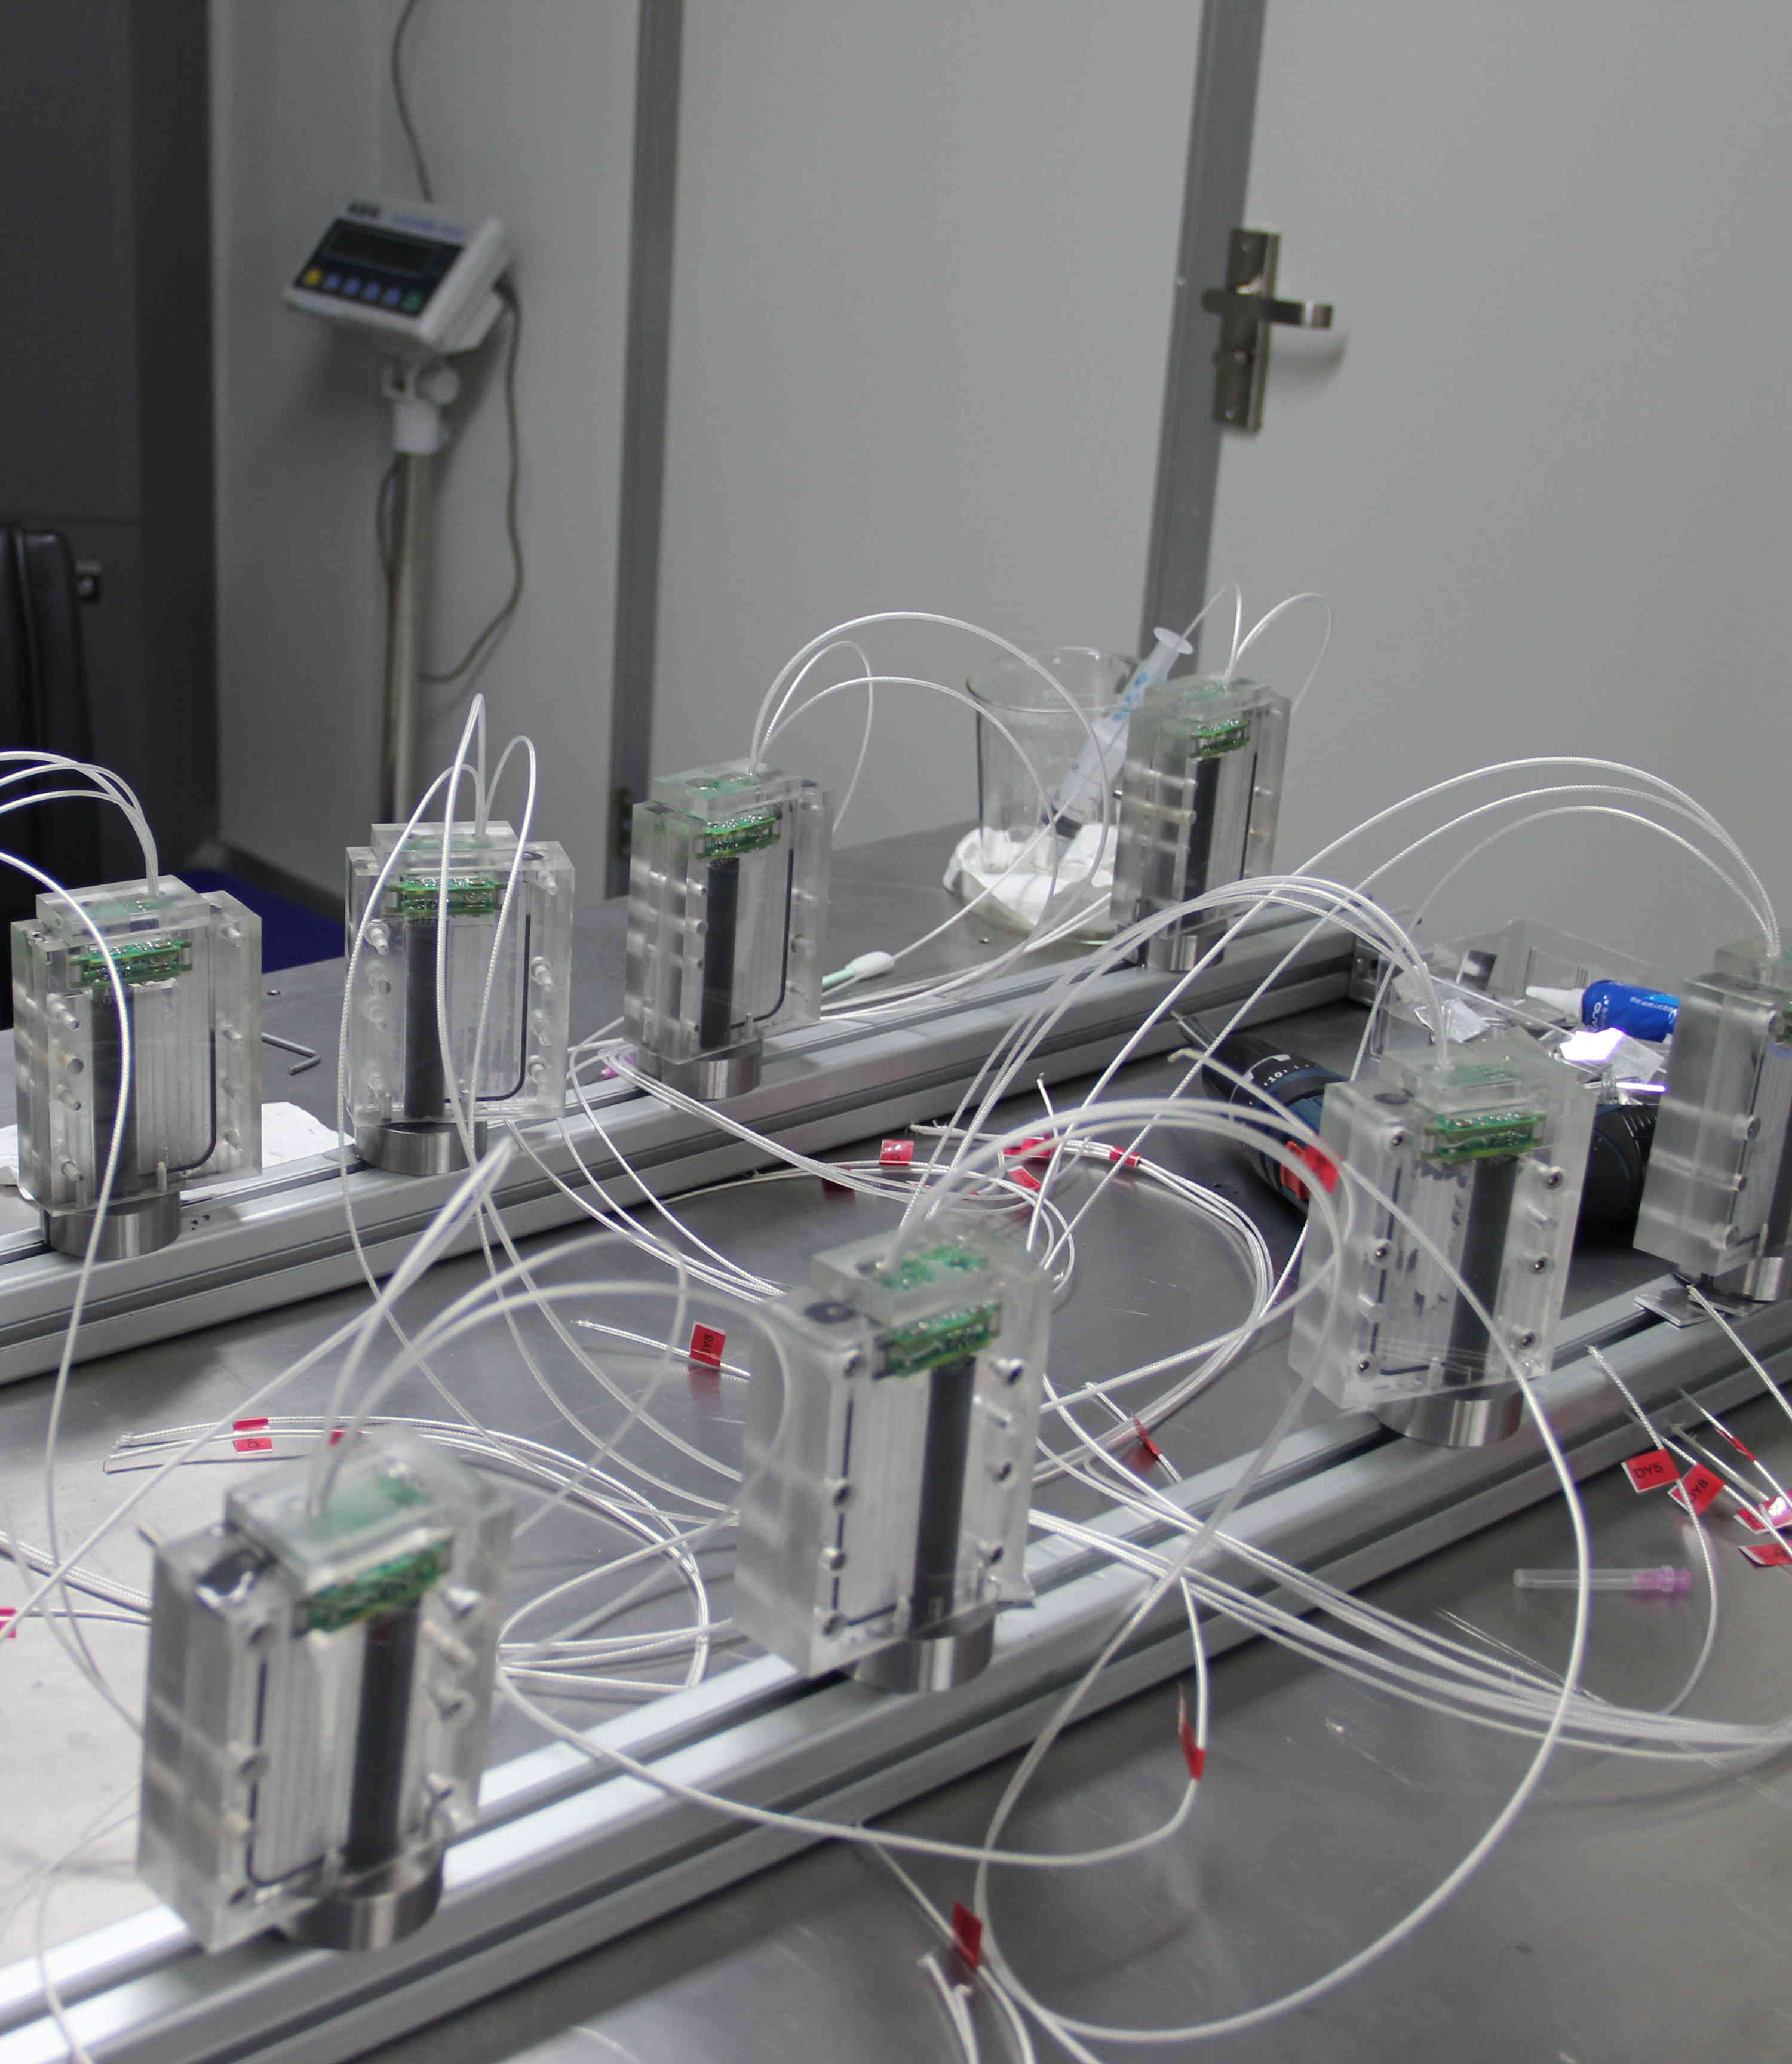
\includegraphics[width=0.32\textwidth]{chap/construction/fig/potting_e.jpg}
}
\subfloat[][完成灌封步骤,拆卸PMT组件]{
	\label{fig:construction:potting_f}
	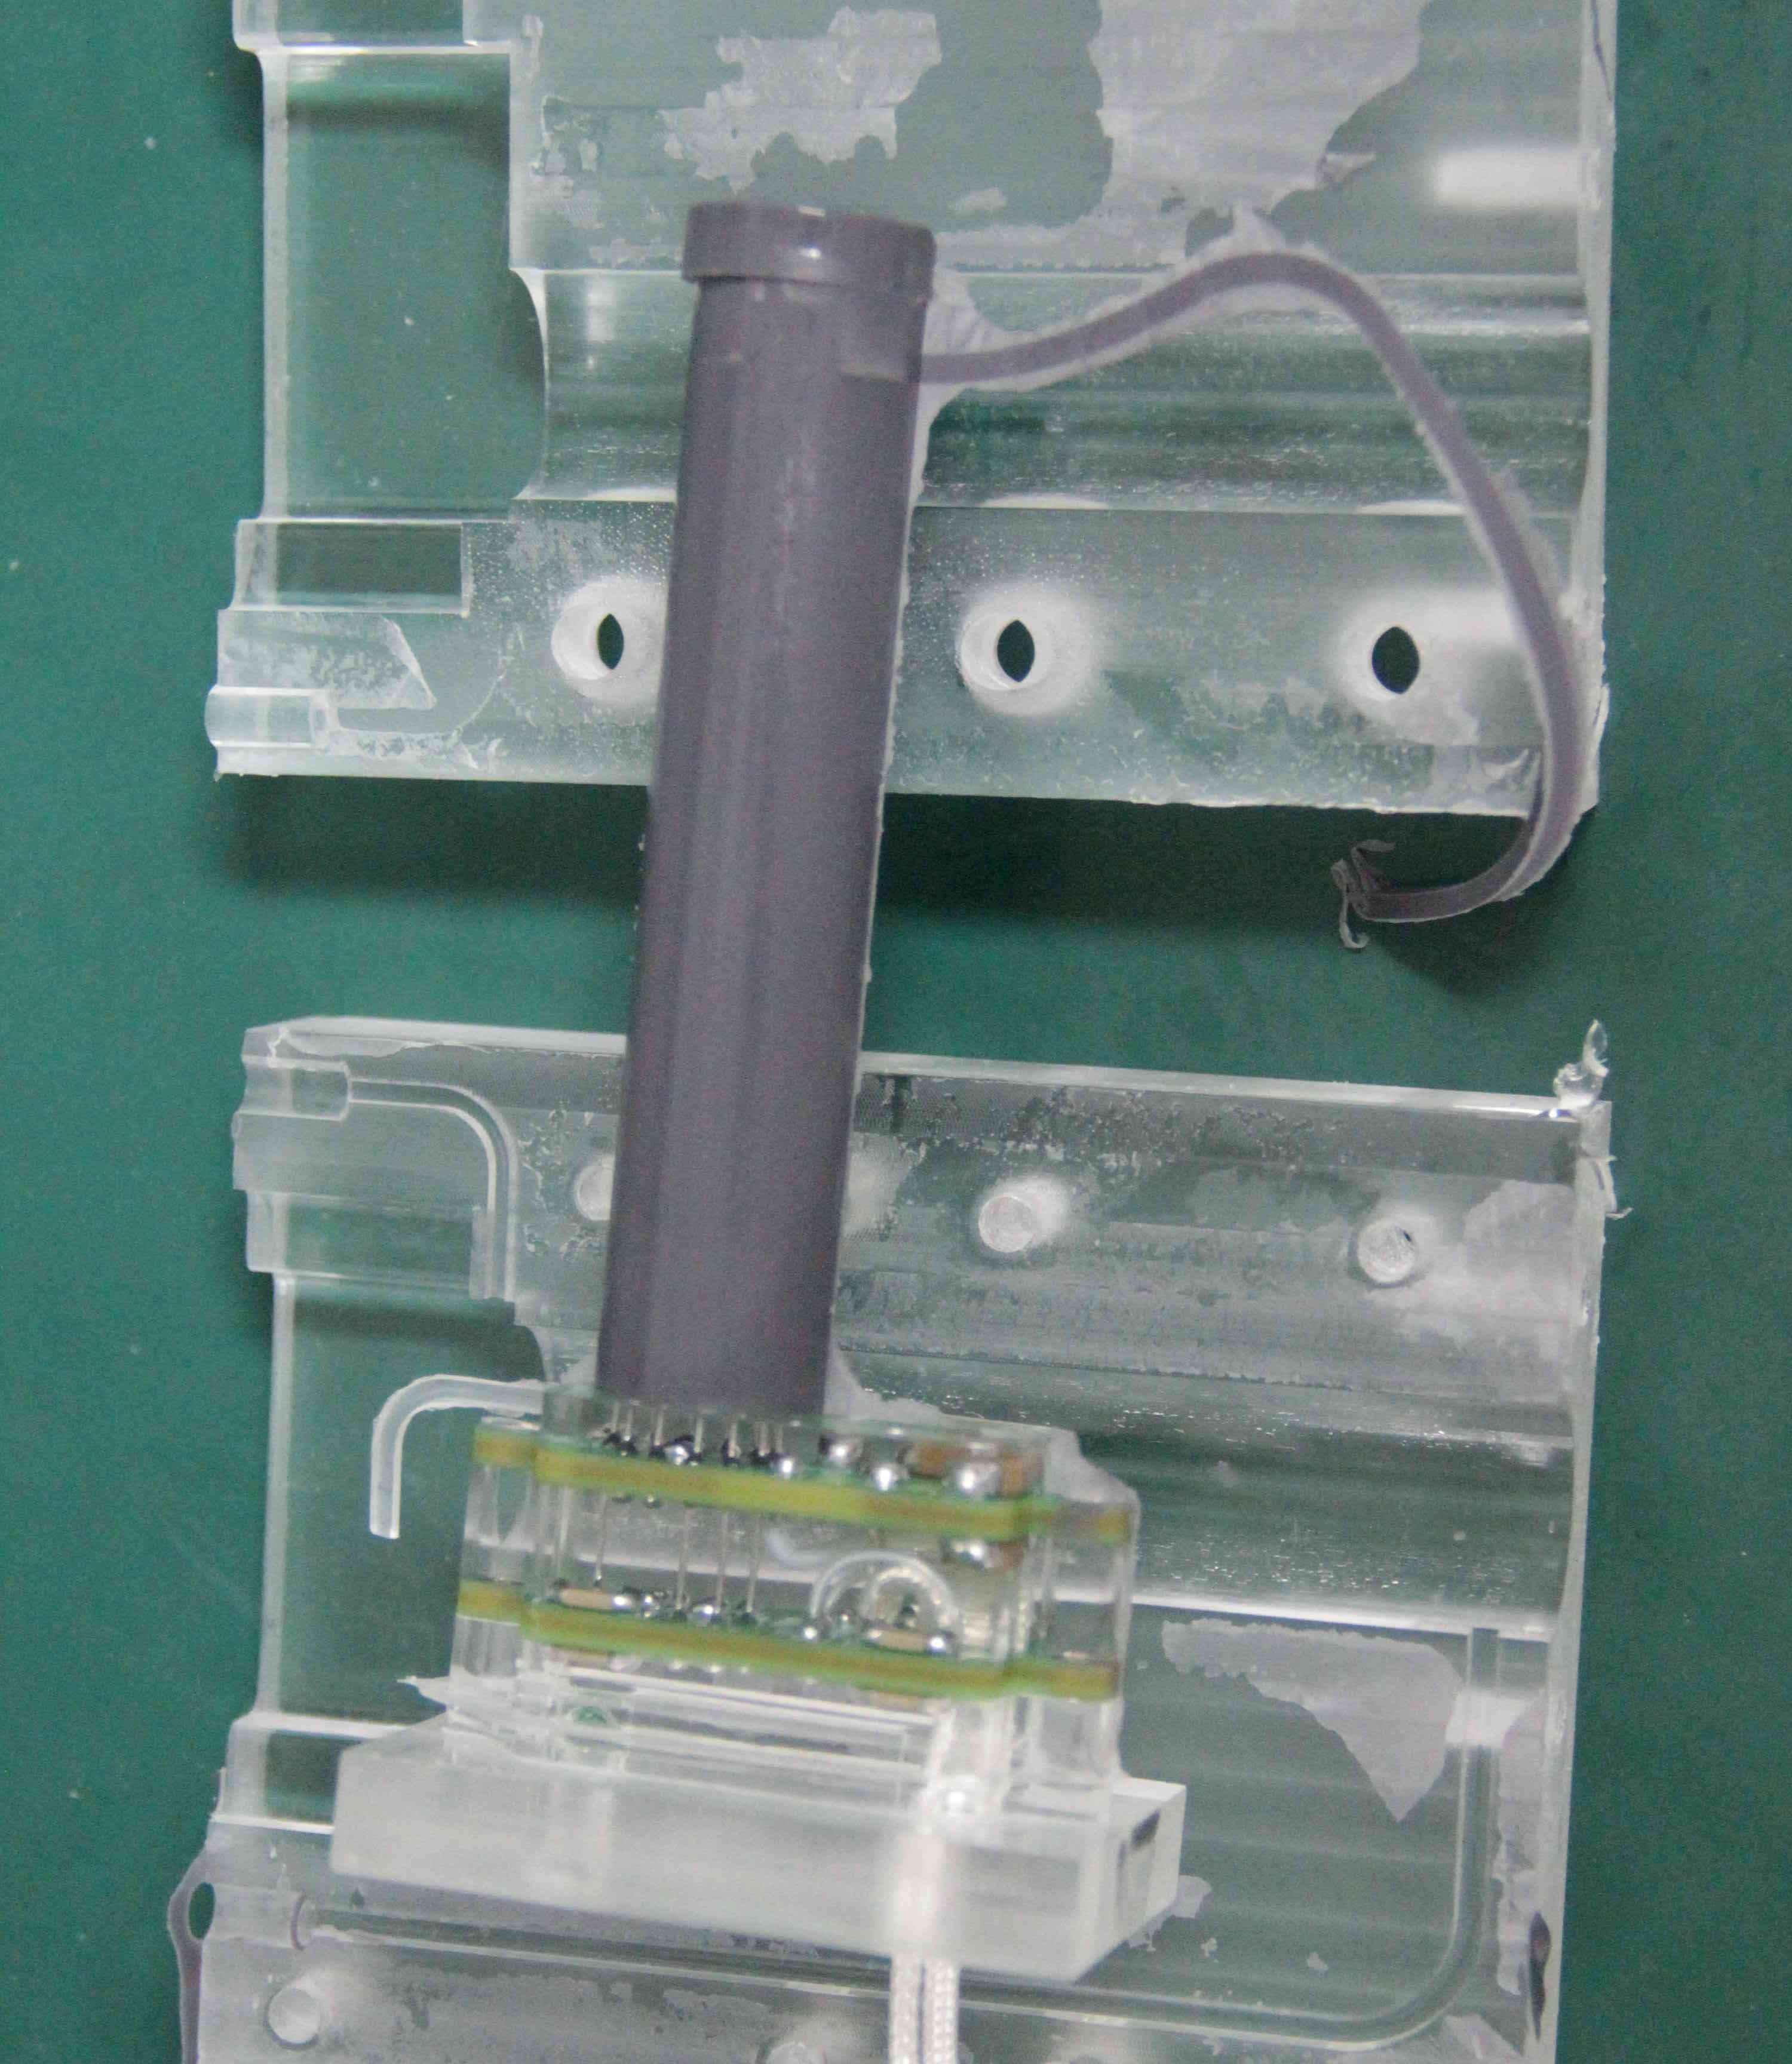
\includegraphics[width=0.32\textwidth]{chap/construction/fig/potting_f.jpg}
}
\caption{PMT组件的灌封操作流程}
\label{fig:construction:potting}
\end{figure}
最后,在灌封结束后,我们将铝合金保护套安装到了PMT组件上,同时给高压线和信号线分别焊上了SHV高压接头和SMA信号接头,这就是PMT组件的装配步骤。
给高压信号线焊上接头是为了方便PSD建造过程中的各种测试,这些接头是临时的,在PSD整体装配时会被剪掉,然后将高压线和信号线直接焊接到高压扇出板和信号转接板上(高压扇出板和信号转接板参看第\ref{ch:description}章)。

% envrioment test
PMT组件的环境试验包含高低温循环测试和真空高压打火测试两项内容。
高低温循环测试时,整个PMT组件被静置在高低温试验箱中,不加电不连线,如图\ref{fig:construction:cycling}所示。
\begin{figure}[htb]
\centering
\subfloat[][高低温试验箱]{
	\label{fig:construction:cycling_a}
	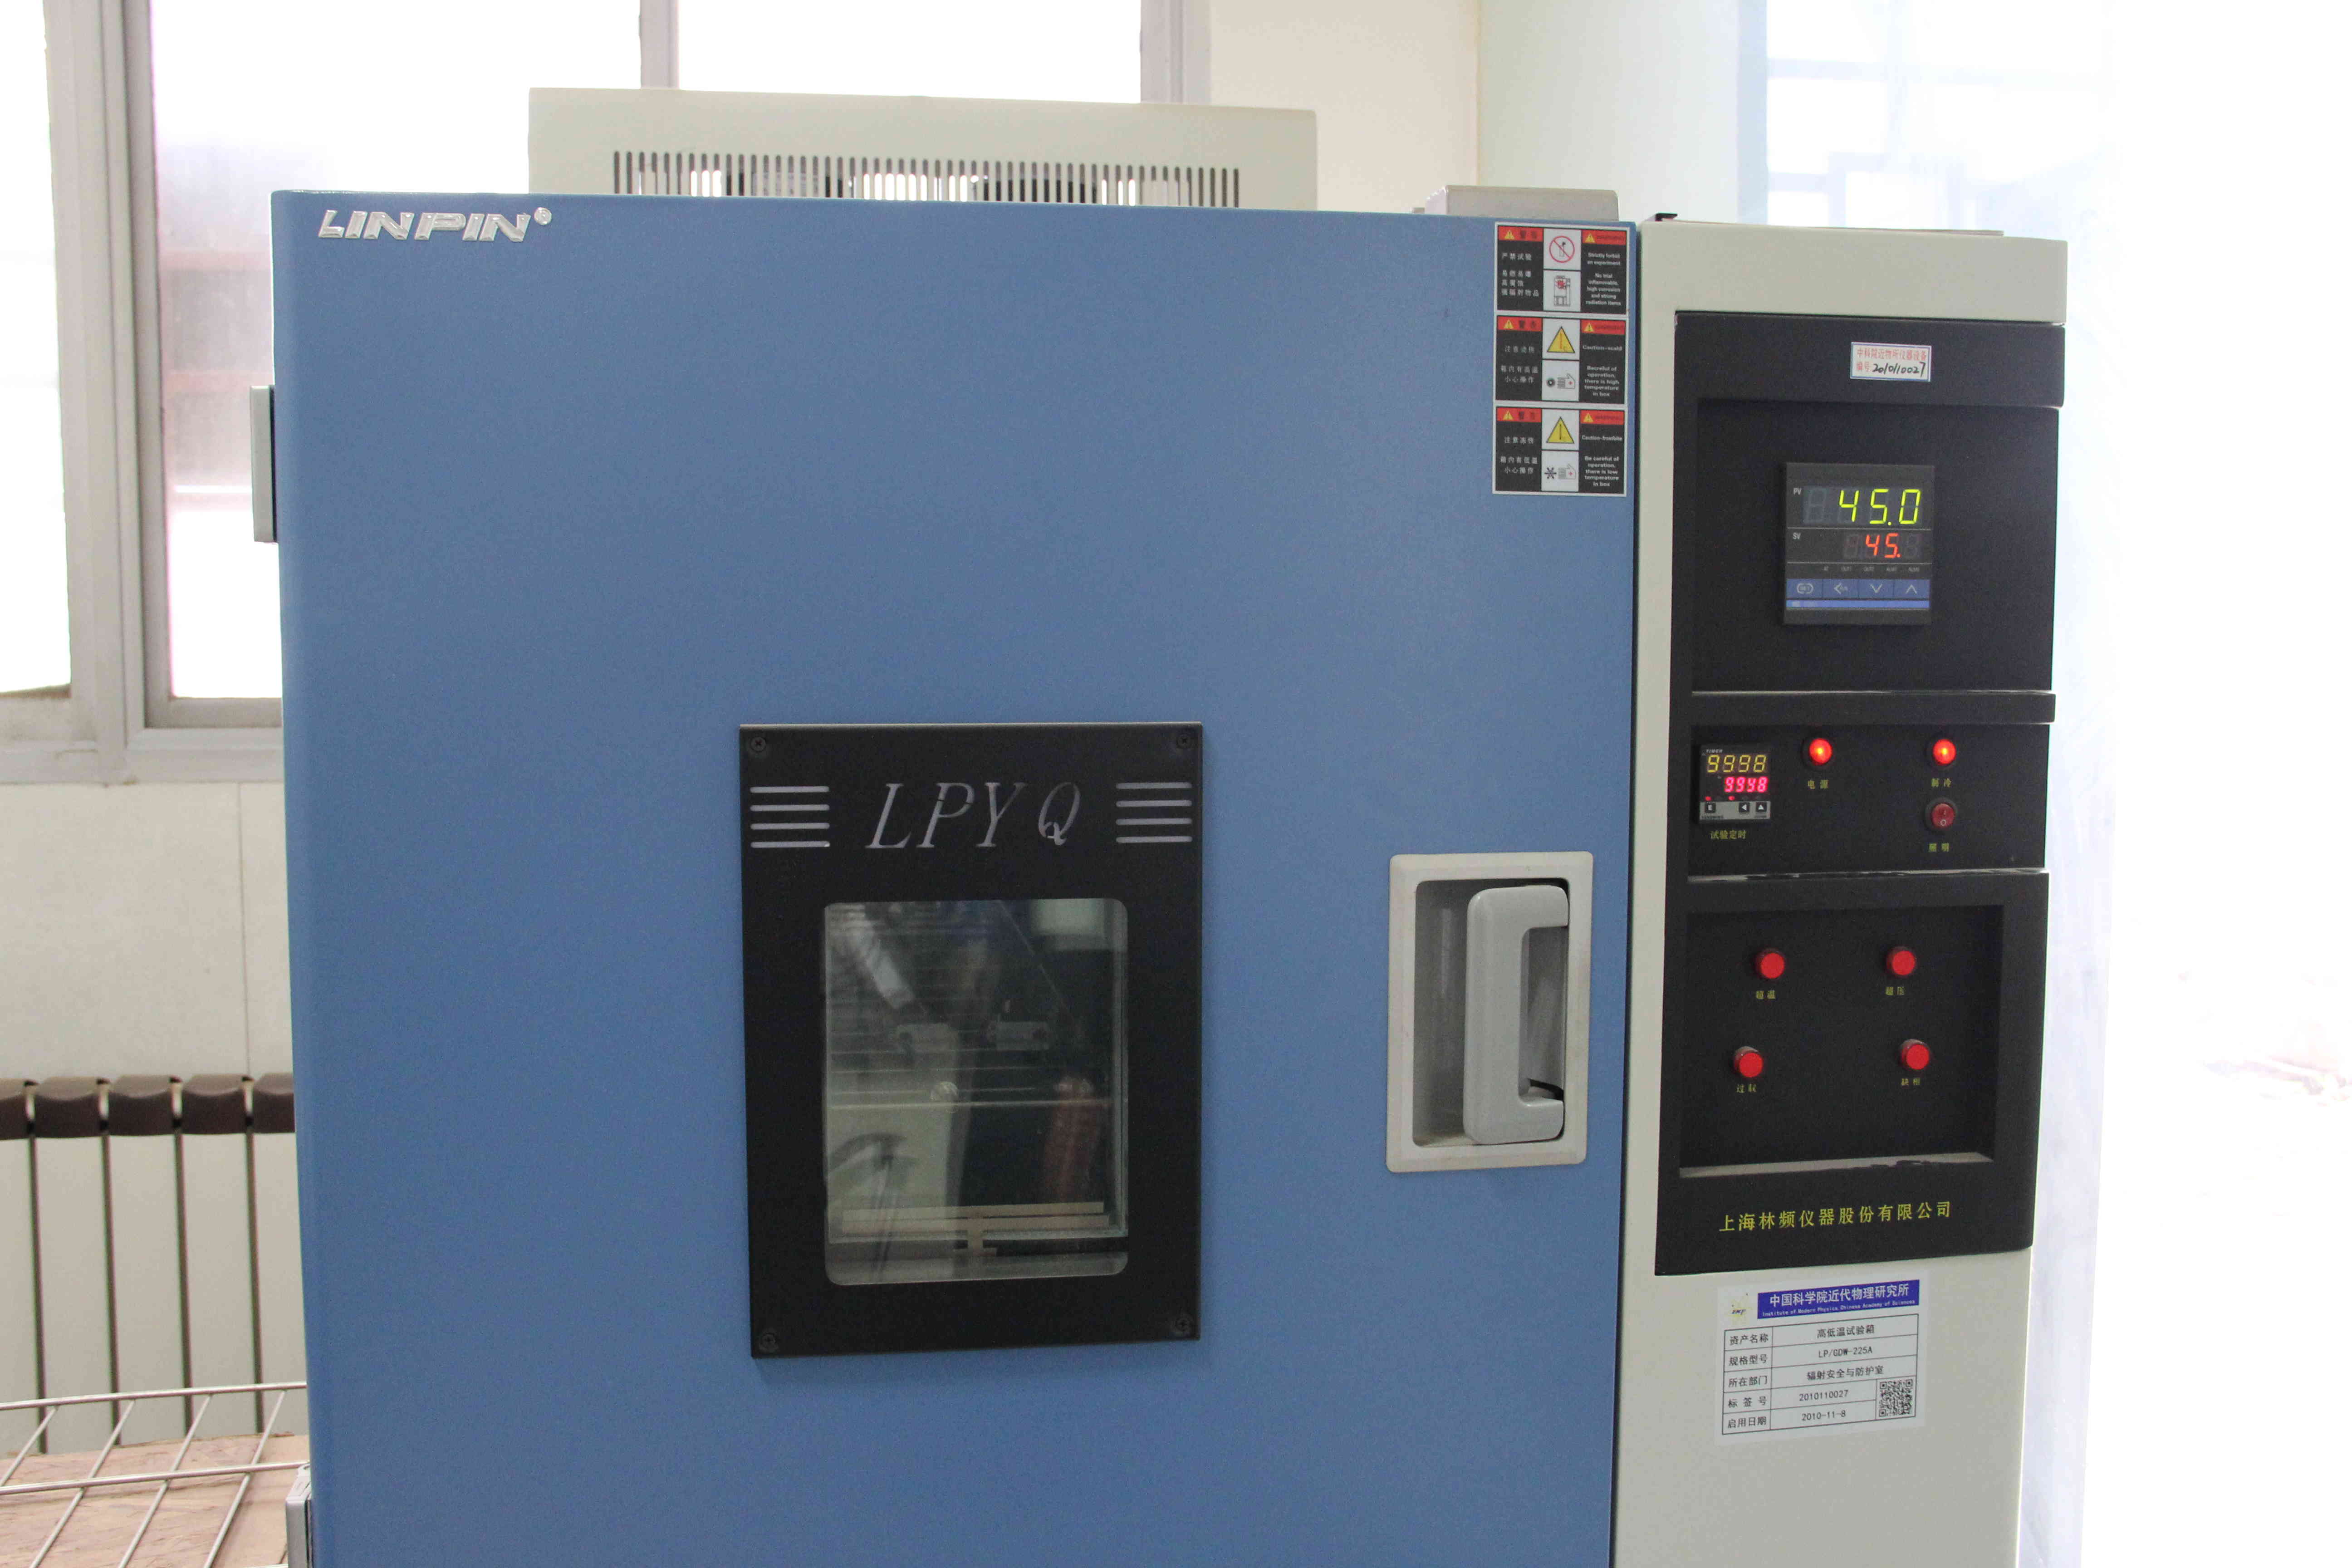
\includegraphics[width=0.48\textwidth]{chap/construction/fig/cycling_a.jpg}
}
% \hfill
\subfloat[][PMT组件静置在高低温试验箱内]{
	\label{fig:construction:cycling_b}
	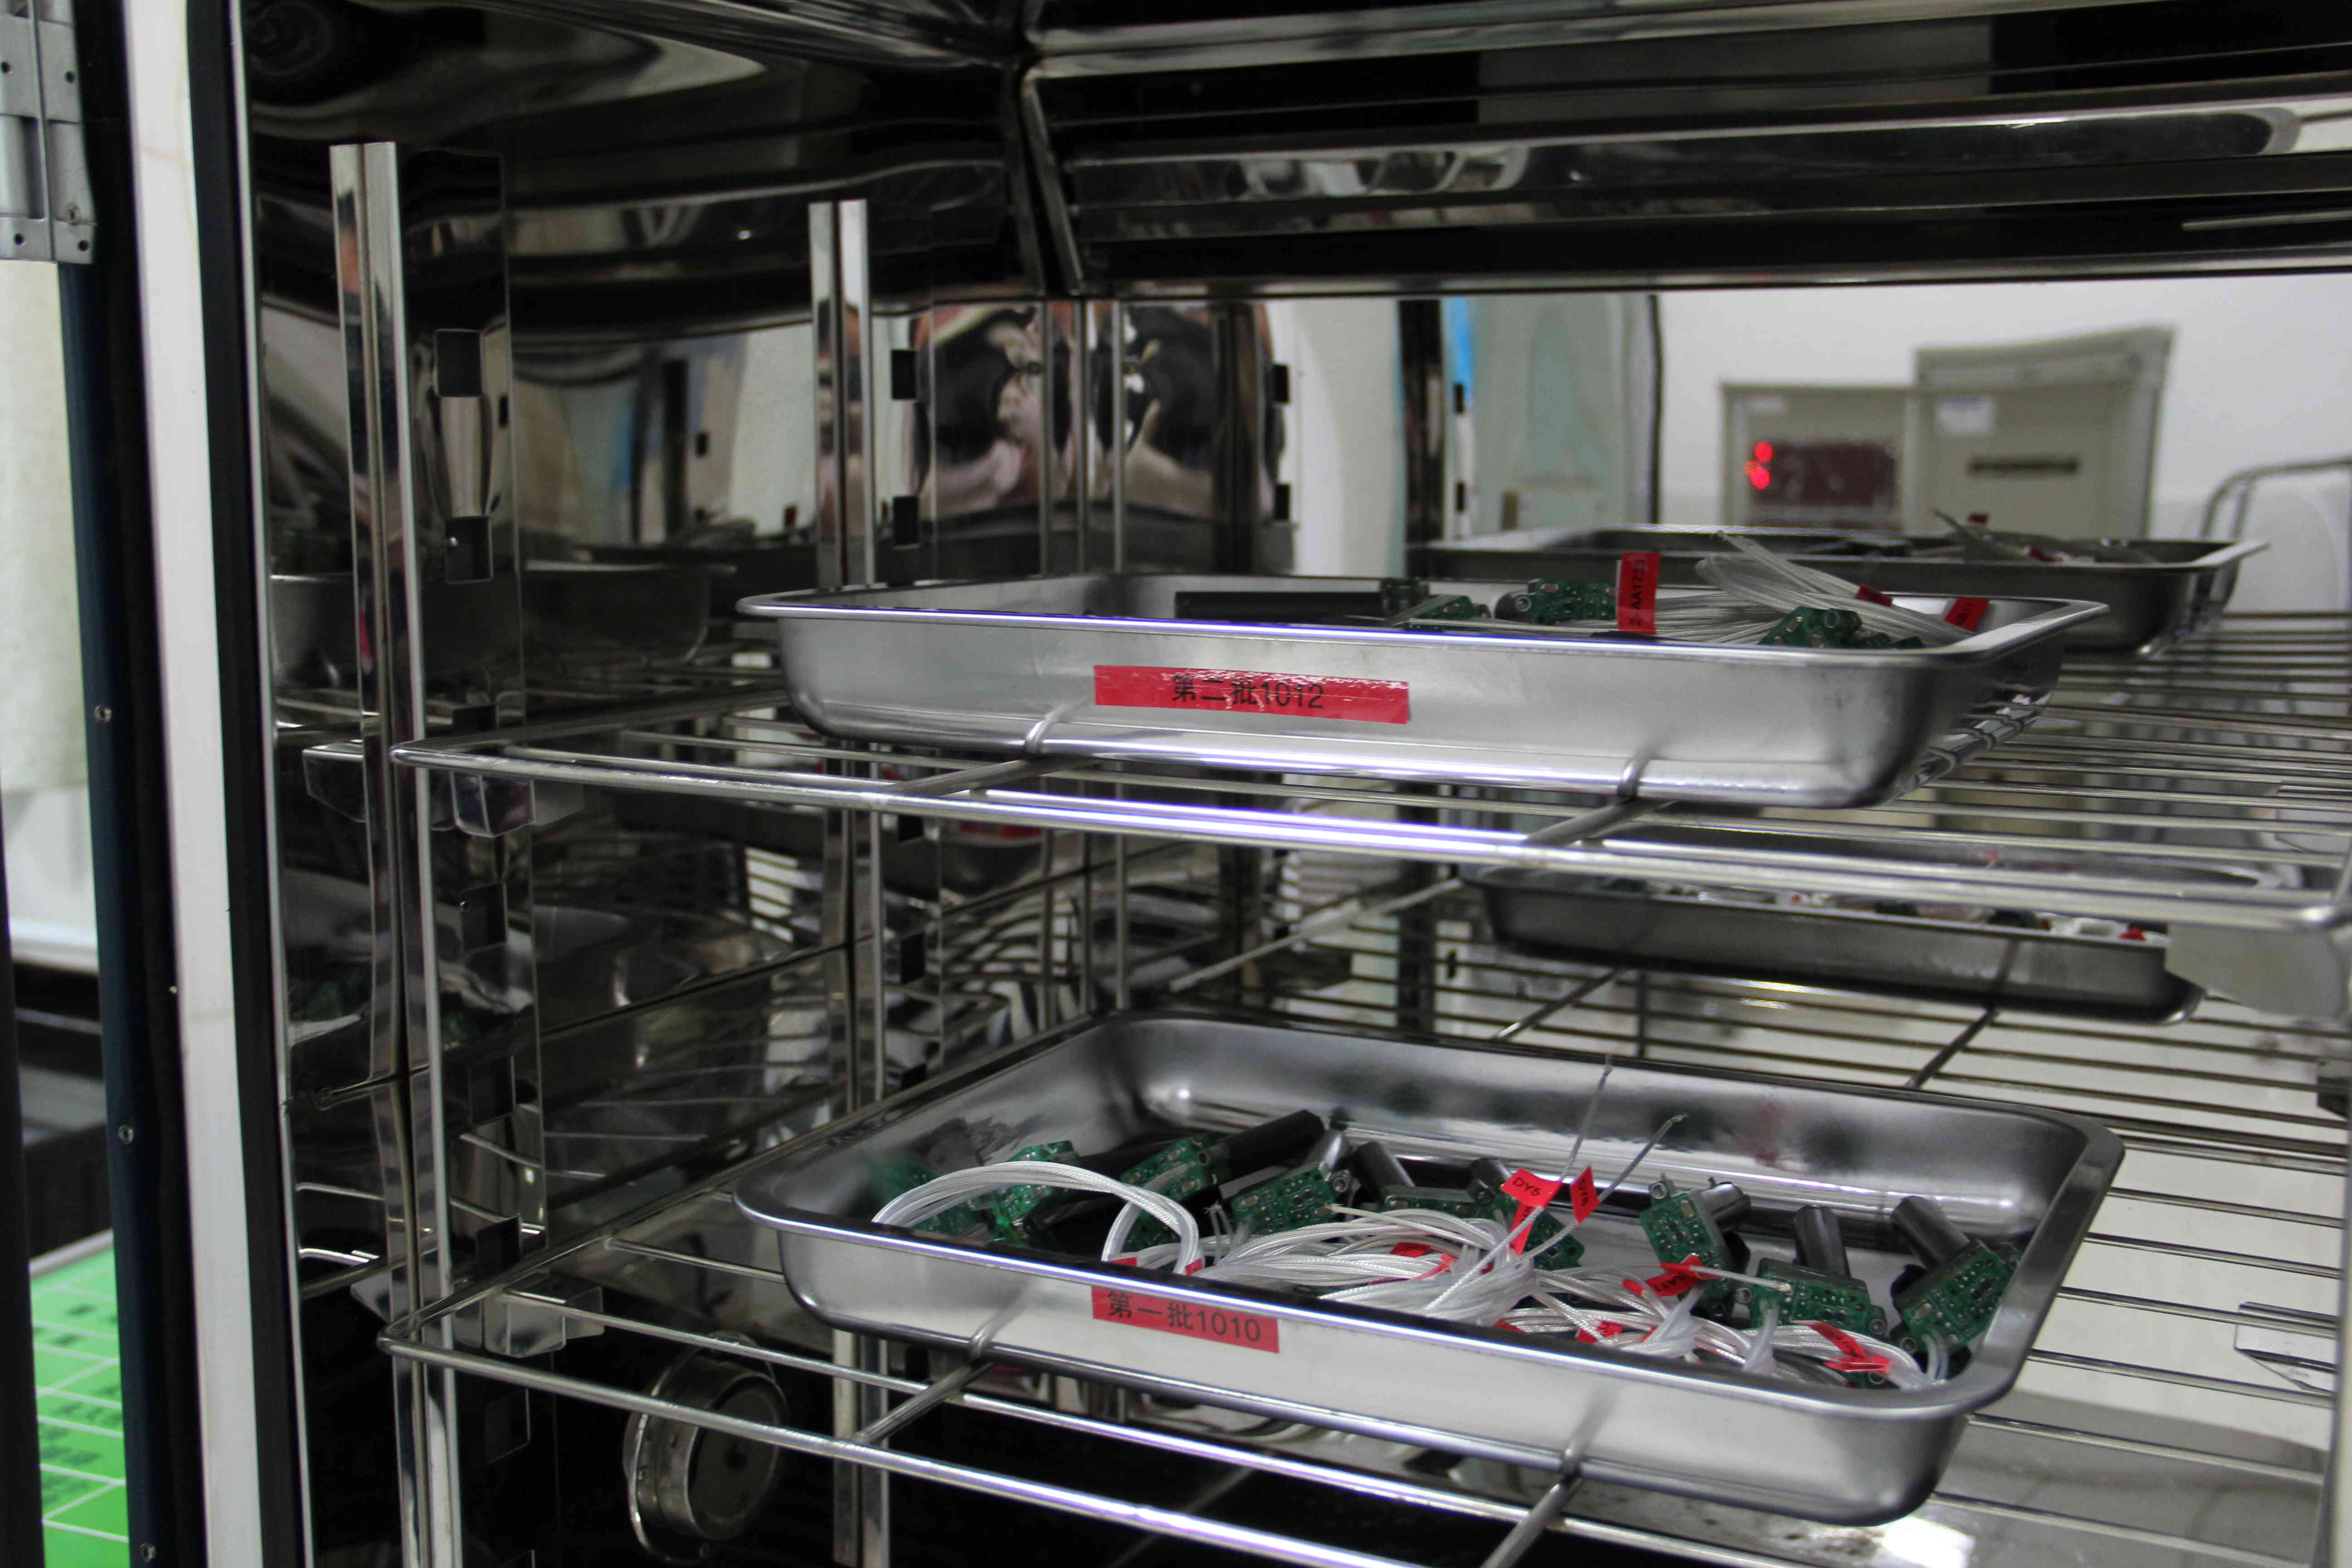
\includegraphics[width=0.48\textwidth]{chap/construction/fig/cycling_b.jpg}
}
\caption{PMT组件的高低温循环测试}
\label{fig:construction:cycling}
\end{figure}
测试一共进行16个循环,每个循环由一个高温和一个低温组成:高温设置为\SI{45}{\celsius},保持1.5个小时;低温设置为\SI{-25}{\celsius},保持2个小时。
这是模拟了DAMPE卫星轨道环境,考察PMT组件在最恶劣的条件下,对频繁高低温度变化的承受能力。
完成高低温测试后,PMT组件马上进行了真空高压打火测试,以考察其在真空中是否会发生高压打火或击穿。
测试使用一个真空靶室来模拟轨道真空环境,靶室使用机械泵抽取真空,并可以通过转接法兰上的SHV双通给内部的PMT组件加载高压。
测试时,使用黑色避光布包裹整个真空靶室一屏蔽外界光干扰,靶室真空度控制在\SI{e-2}{mbar}左右,然后给PMT组件Base板加上\SI{1000}{V}的正高压。
正常情况下,高压通道上的反馈电流应该等于并稳定保持在Base上的微小分压器电流;而发生高压打火或击穿时,反馈电流瞬间变大,并且恢复不到之前的微小数值。
我们认为,合格的PMT组件应该在上述工作状态下至少保持1个小时以上而不发生高压打火事件。

% qualification
上述环境试验完成后,我们再一次对PMT组件的电阻电容值进行了检查,通过与之前PMT组件焊接完成后的阻容值进行对比,可以初步判断PMT组件的Base电路板是否在上述环境试验中受到损伤。
为了进一步考察PMT组件整体的功能完整性,我们使用PMT批量测试平台对PMT组件在额定工作档位下的相对增益和Dy58比值进行了测量,这就是PMT组件的质量鉴定测试。
该测试具有两个目标:1)测试PMT组件是否能够正常工作,其性能指标是否在合理范围内,这是PMT组件质量是否合格的最终测试指标;2)得到最终的PMT组件相对增益一致性和Dy58比值一致性,确认前面的PMT筛选没有问题。
PMT组件中已经在R4443端面上耦合了一层硅脂垫片,而垫片端面又有一层塑料保护膜,这层保护膜只有在将PMT组件安装到PSD上时才能够去掉。
这些都会影响到此次测试的结果,因此我们不期望测试结果与PMT性能测试的结果完全一致,只要PMT组件没有出现极端异常的结果,我们都认为是正常的。
图\ref{fig:construction:qualification_result}给出了PMT组件质量鉴定测试的结果,可以看到所有PMT组件的性能参数都分布在合理的区间内。。
\begin{figure}[htb]
\centering
\subfloat[][PMT组件的增益分布]{
	\label{fig:construction:amp_dist_afterpotting}
	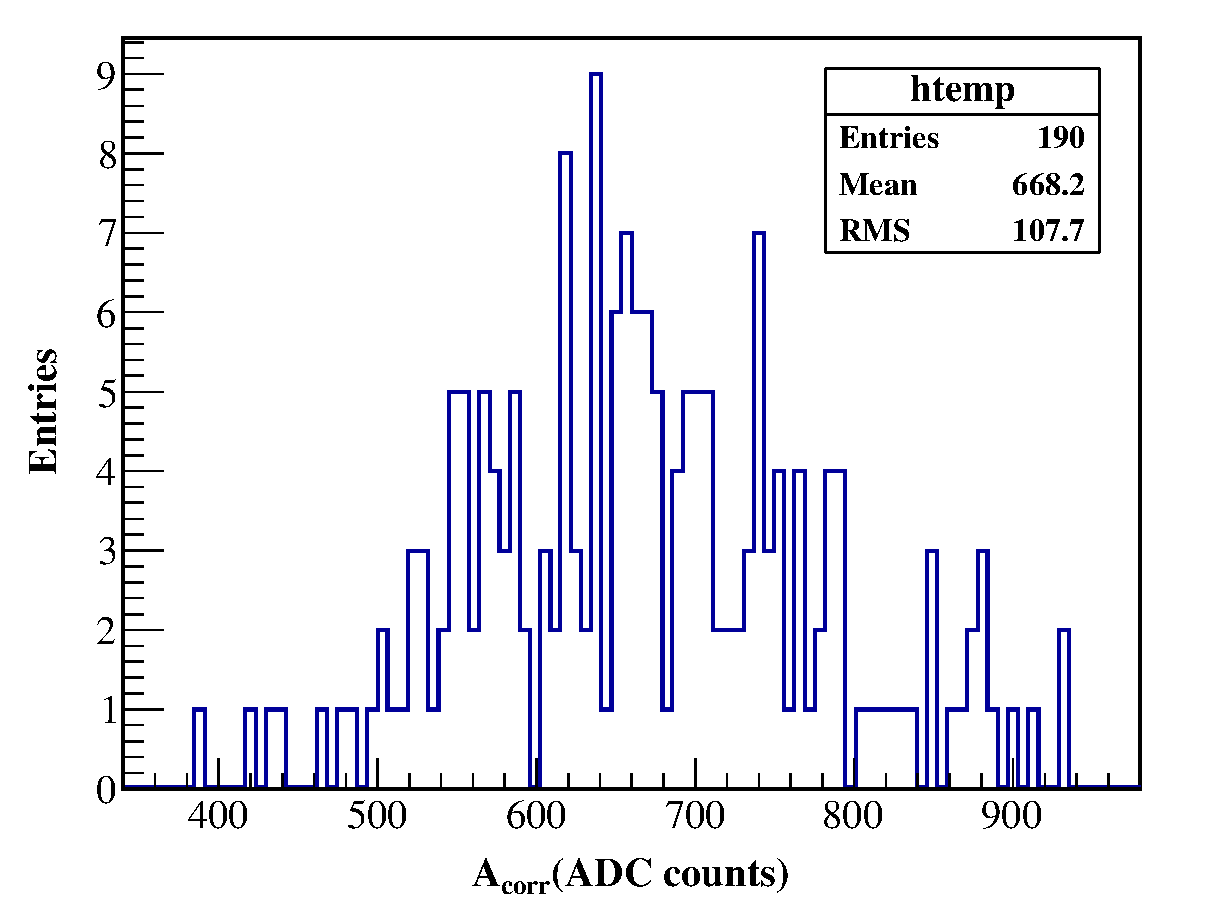
\includegraphics[width=0.48\textwidth]{chap/construction/fig/amp_dist_afterpotting.eps}
}
% \hfill
\subfloat[][PMT组件的Dy58比值分布]{
	\label{fig:construction:dy58_dist_afterpotting}
	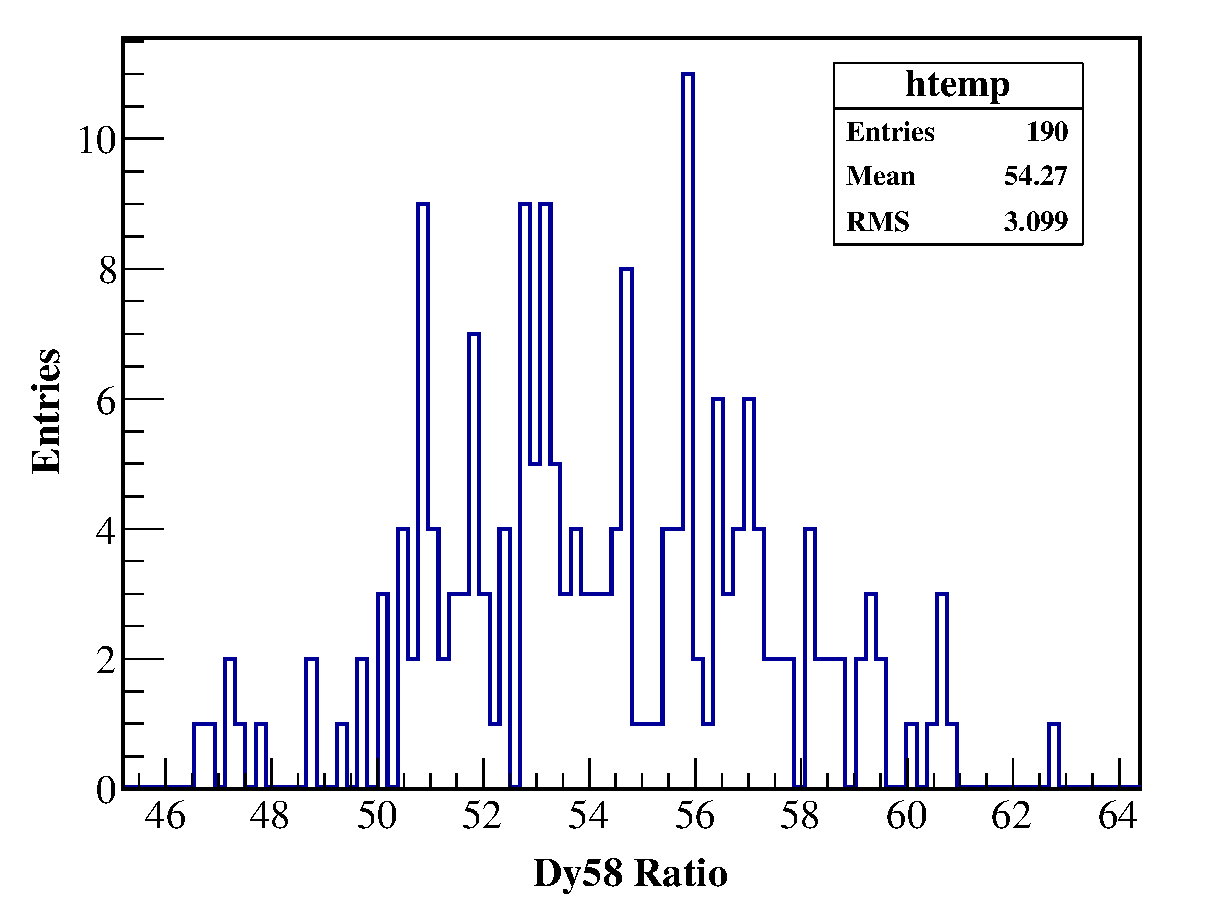
\includegraphics[width=0.48\textwidth]{chap/construction/fig/dy58_dist_afterpotting.eps}
}
\caption{PMT组件的质量鉴定测试结果}
\label{fig:construction:qualification_result}
\end{figure}

\section{塑闪单元条组件的生产}
\label{sec:construction:bar_production}

\subsection{单元条的包装与测试}
\label{sec:construction:bar_wrapping_and_test}

塑闪单元条组件的生产流程如图\ref{fig:construction:bar_production}所示。
\begin{figure}[htbp]
	\centering
	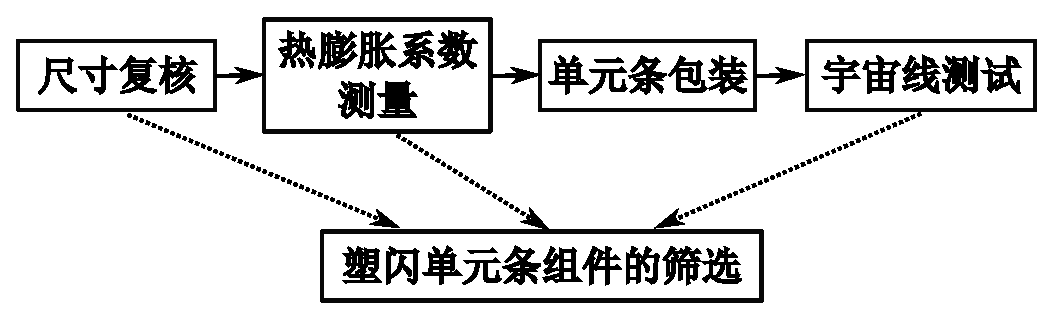
\includegraphics[width=0.65\textwidth]{chap/construction/fig/bar_production.eps}
	\caption{塑闪单元条组件的生产流程}
	\label{fig:construction:bar_production}
\end{figure}
首先,我们对裸塑闪单元条的尺寸进行了测量,同时检查其外观是否完好无损。PSD的结构设计对单元条的尺寸提出了严格要求,正式安装的单元条必须满足设计图纸的公差尺寸。
其次,我们对这些塑闪单元条进行了热膨胀系数的测量。这是因为PSD在结构上采用了活动端设计来释放塑闪单元条温度形变应力(详见\ref{sec:description:psd_support}节),同一层的41根单元条之间的热膨胀系数不能相差太大,以致形变应力全部堆积在一根或若干根单元条上。
测试在中航工业兰州飞行控制有限公司的大型高低温试验箱中进行,共对4个不同温度(\SI{-20}{\celsius},\SI{0}{\celsius},\SI{20}{\celsius},\SI{40}{\celsius})下单元条的长度进行了测量,从而得到了每根条子的热膨胀系数。
\begin{figure}[htbp]
	\centering
	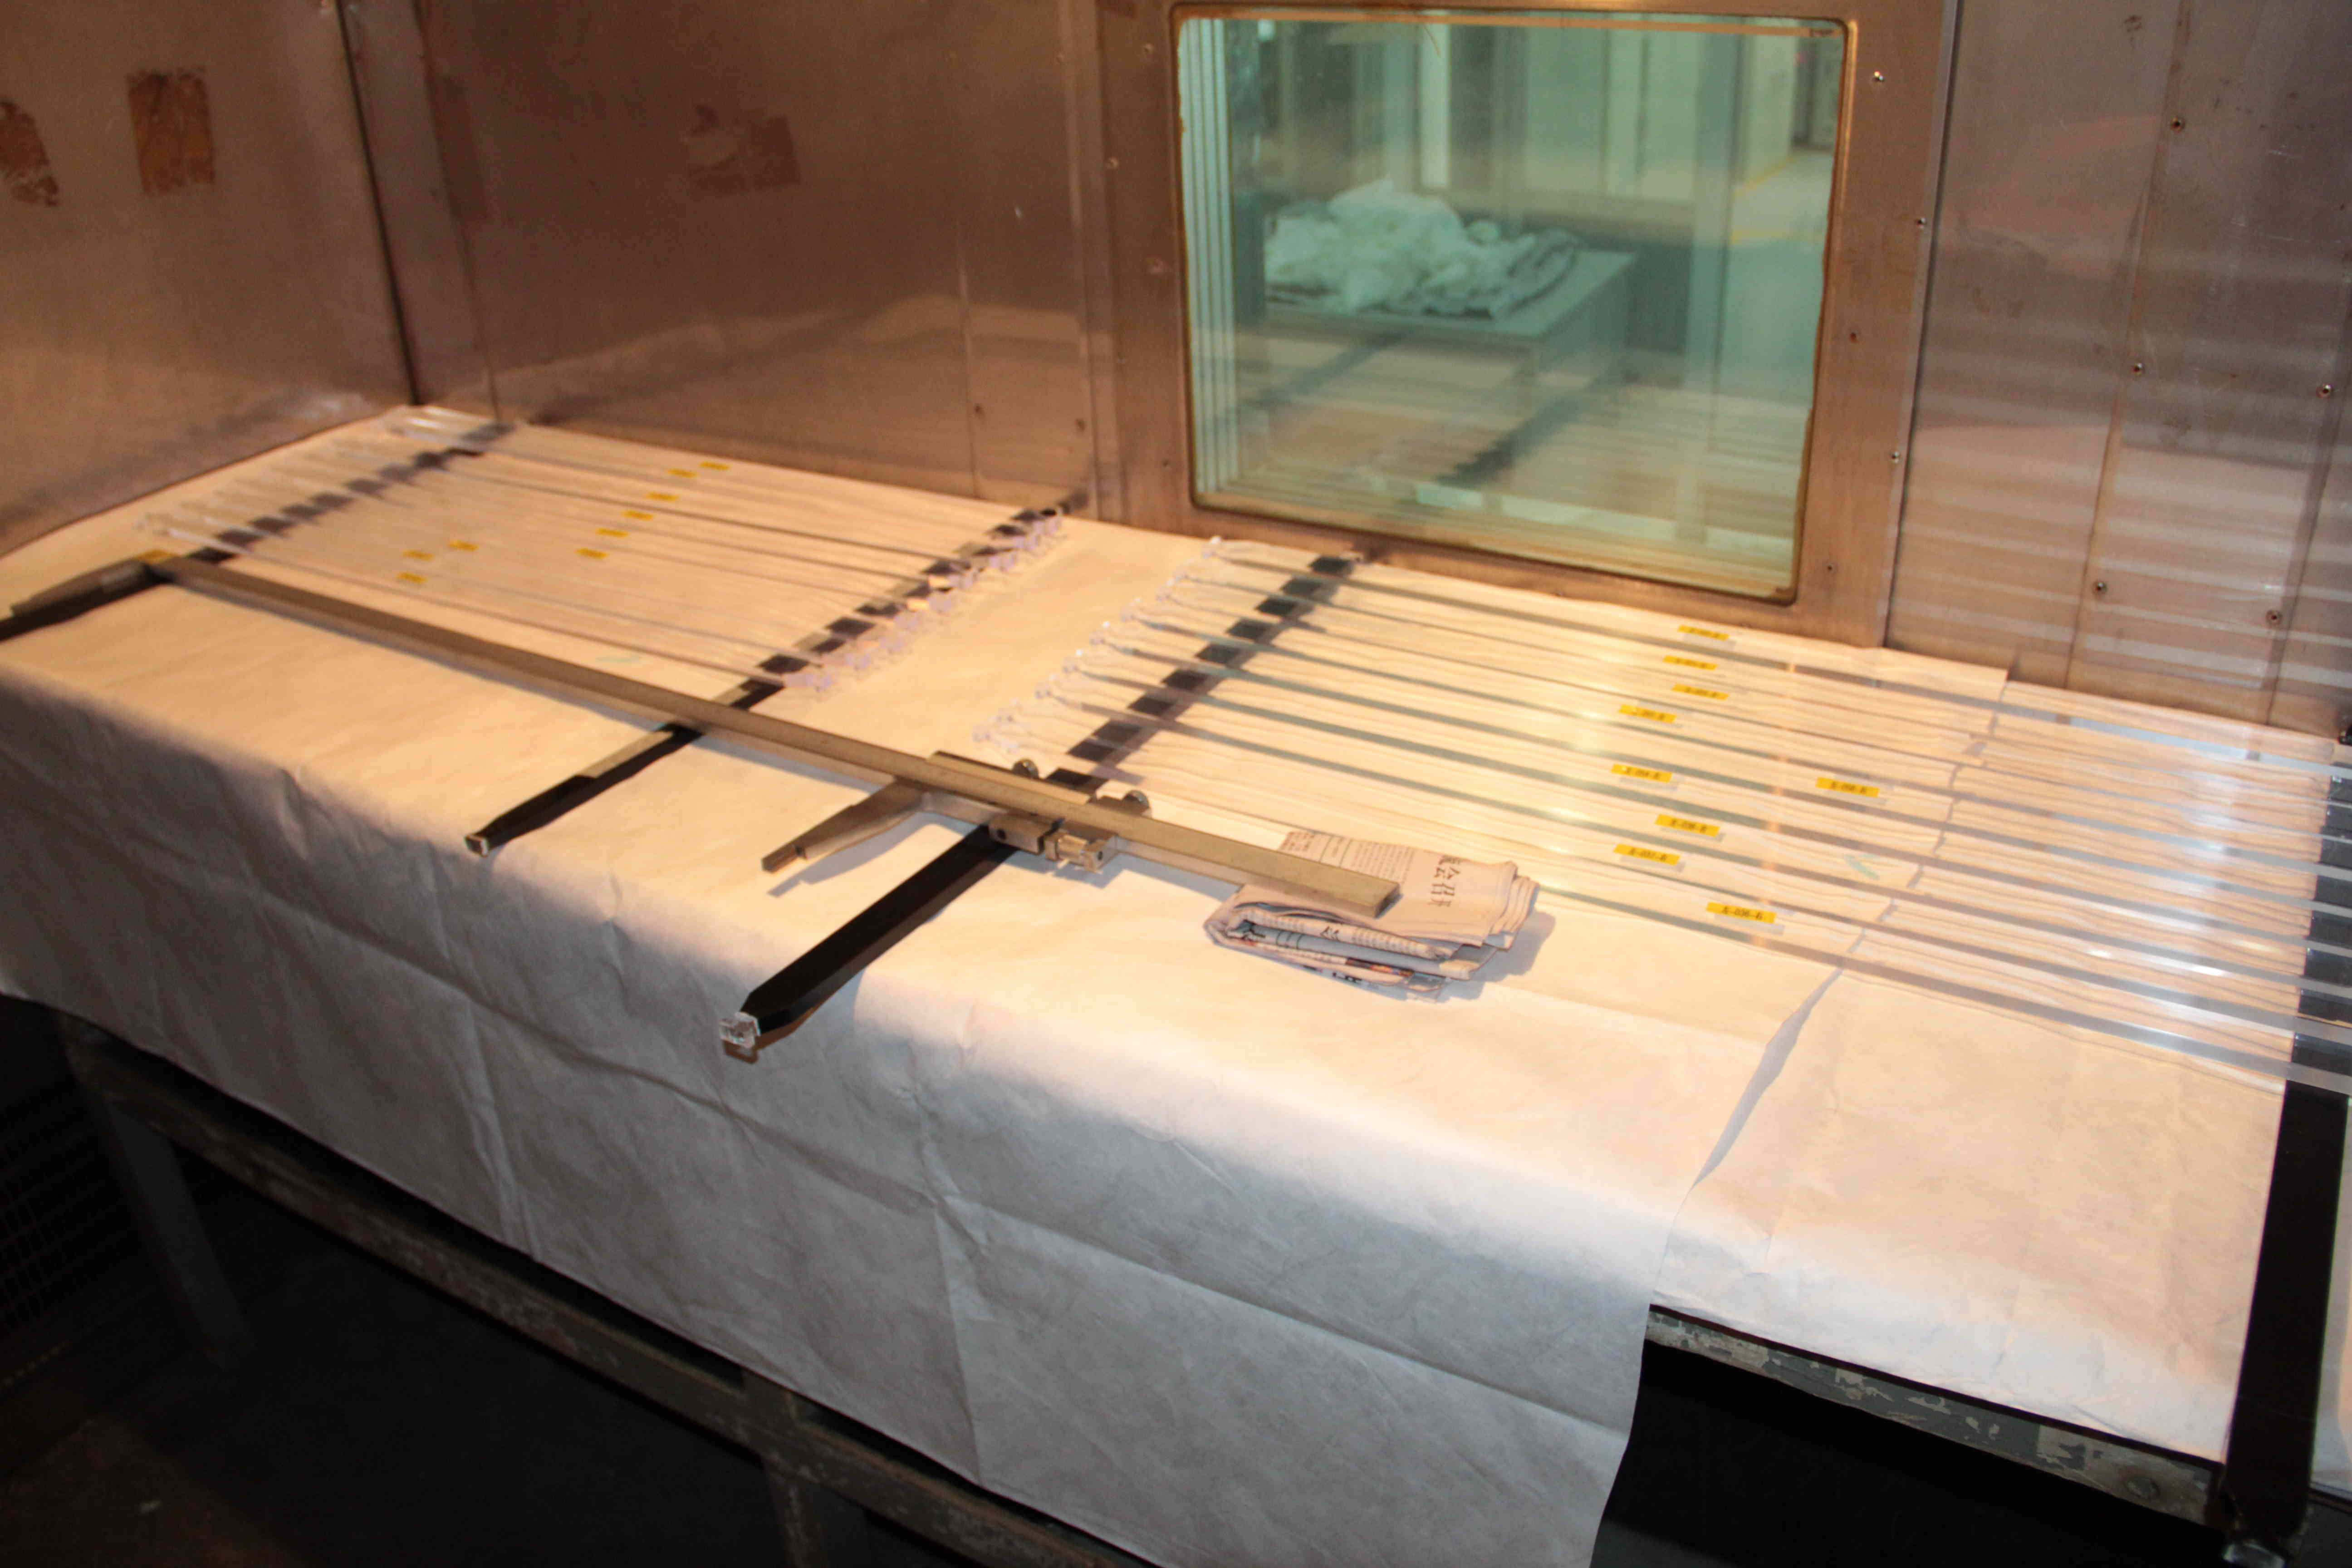
\includegraphics[width=0.65\textwidth]{chap/construction/fig/bar_cylcling.jpg}
	\caption{塑闪单元条的热膨胀系数测试}
	\label{fig:construction:bar_cylcling}
\end{figure}
在每个温度点,在单元条的形变稳定后,测试人员进入试验箱内部进行测量操作,所有测量完成后再切换到下一个温度点。
为了保证测量结果的准确性,我们把测量长度用的游标卡尺也放进高低温试验箱中,跟随被测单元条一起经历温度变化,如图\ref{fig:construction:bar_cylcling}所示。


之后,我们对裸单元条进行了正式包装。
\begin{figure}[htb]
\centering
\subfloat[][]{
	\label{fig:construction:bar_wrapping_a}
	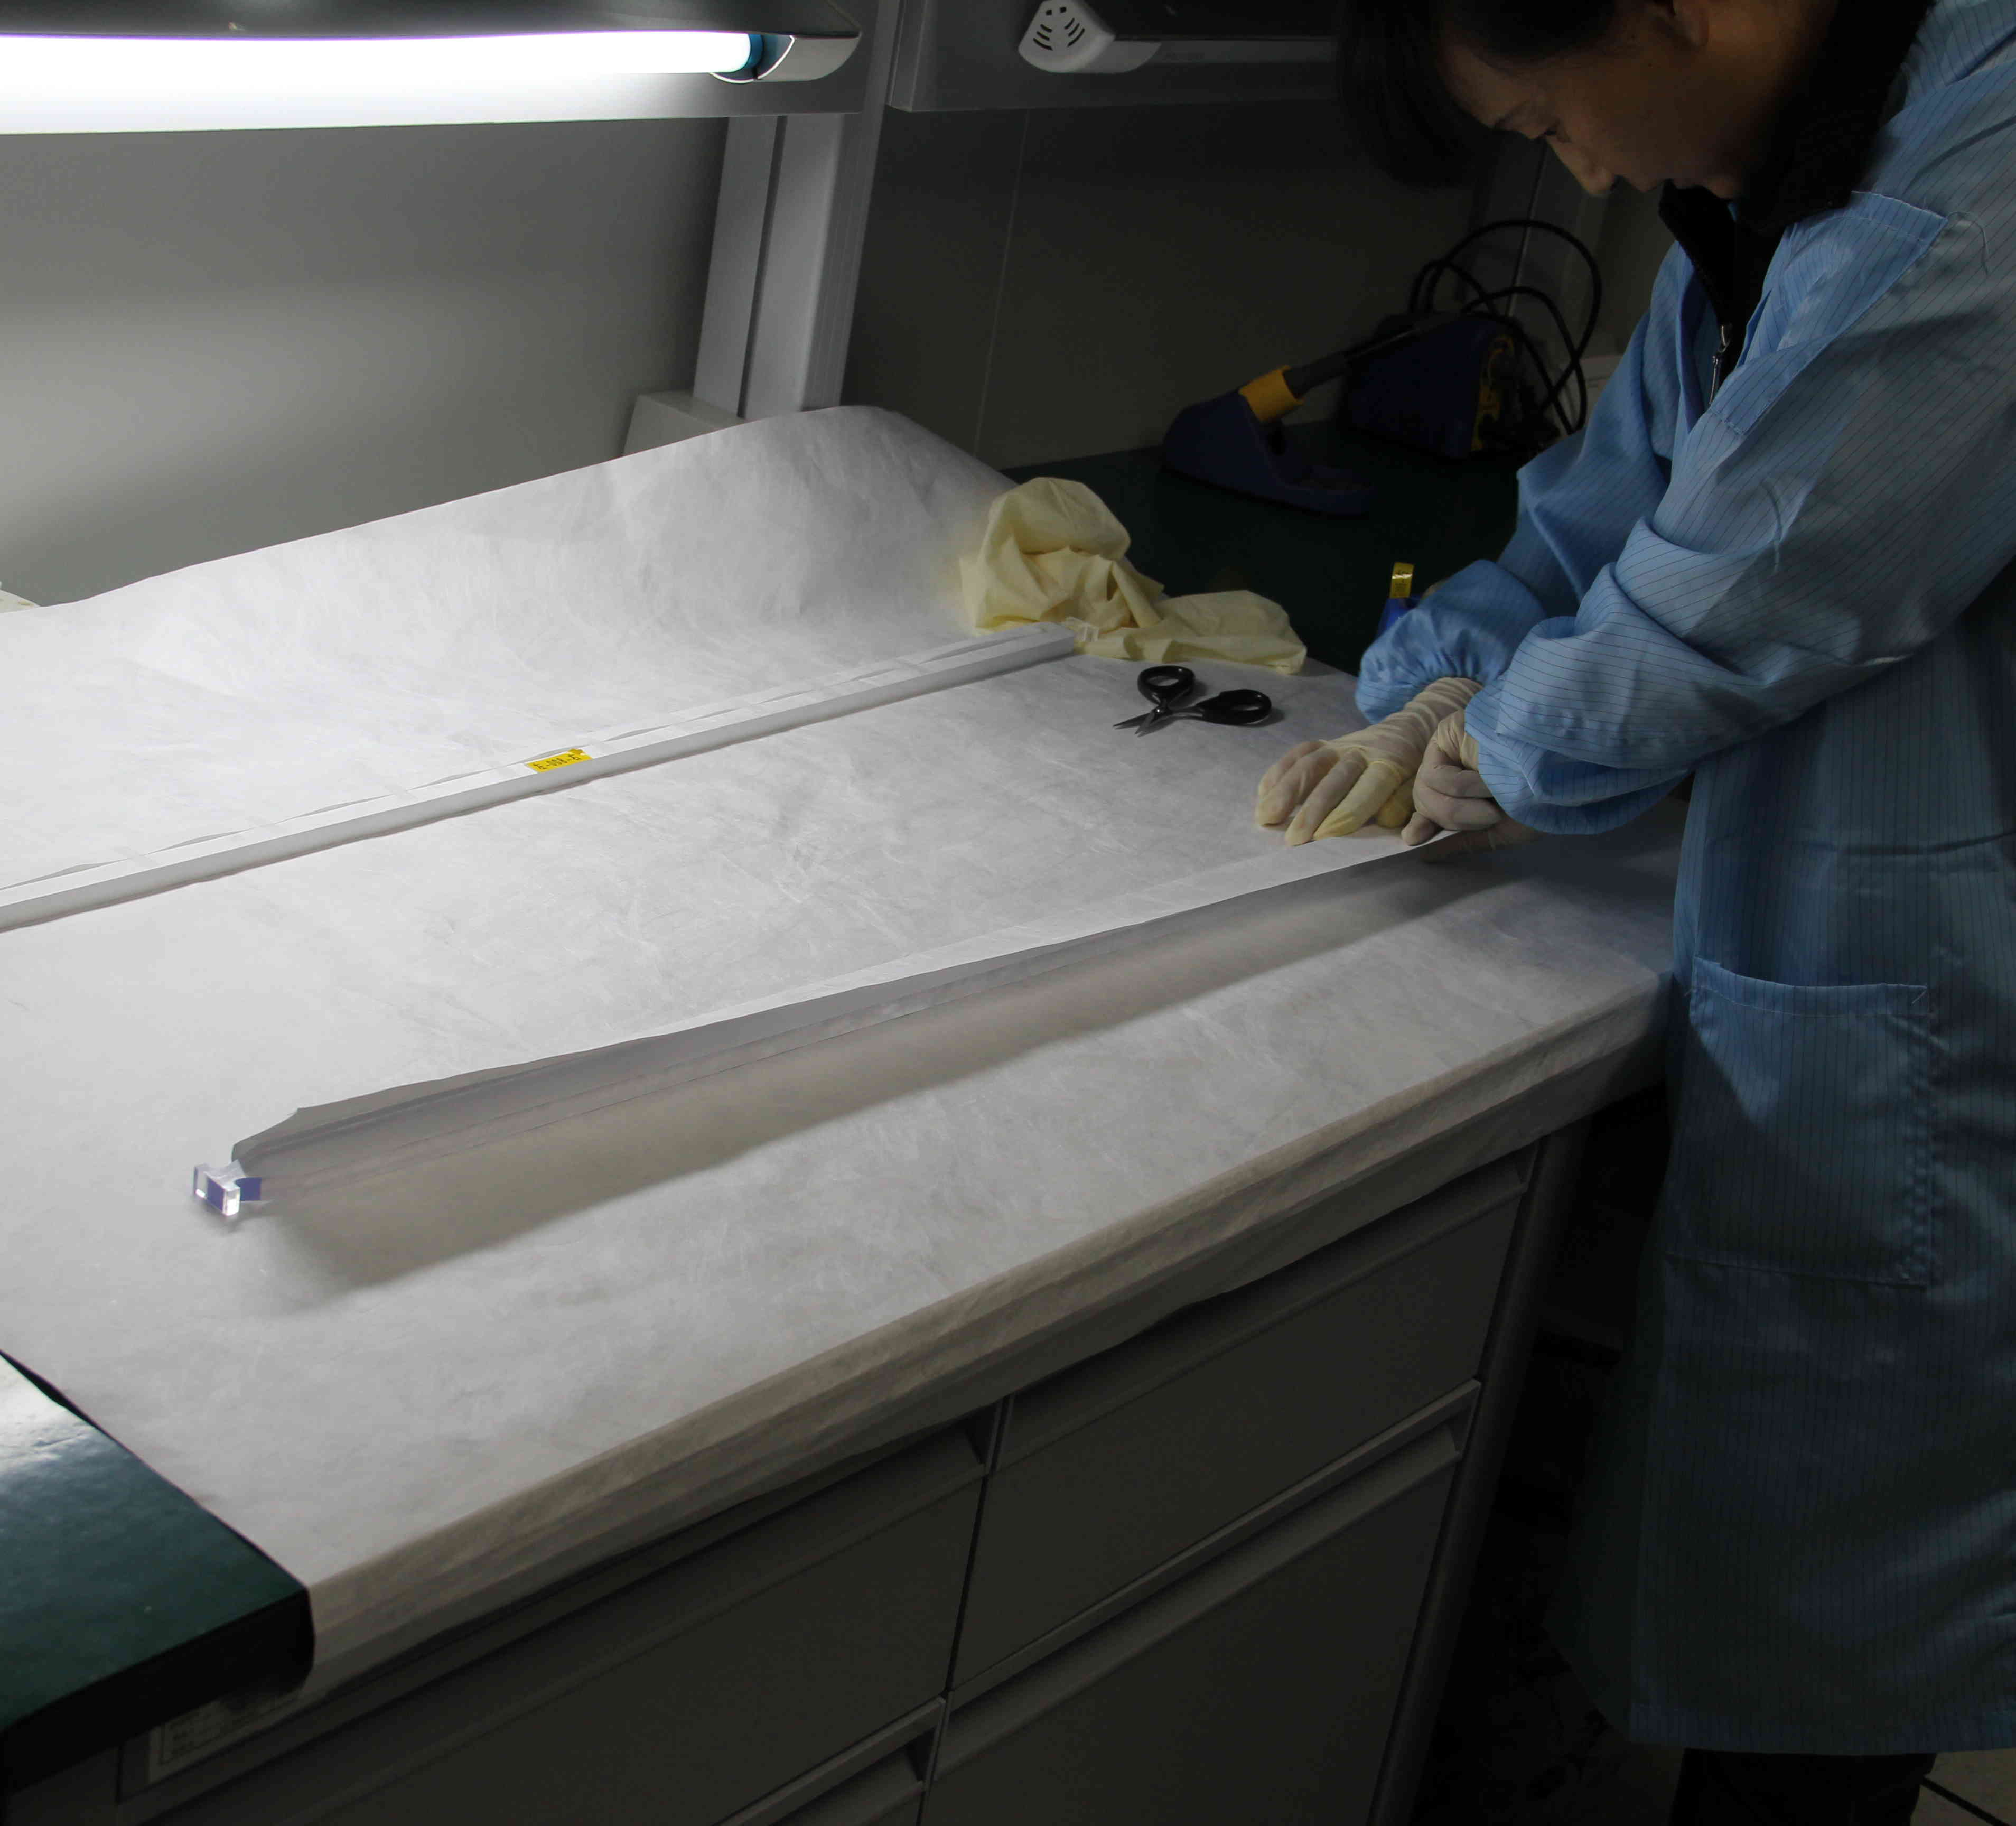
\includegraphics[width=0.25\textwidth]{chap/construction/fig/wrapping_a.jpg}
}
\subfloat[][]{
	\label{fig:construction:bar_wrapping_b}
	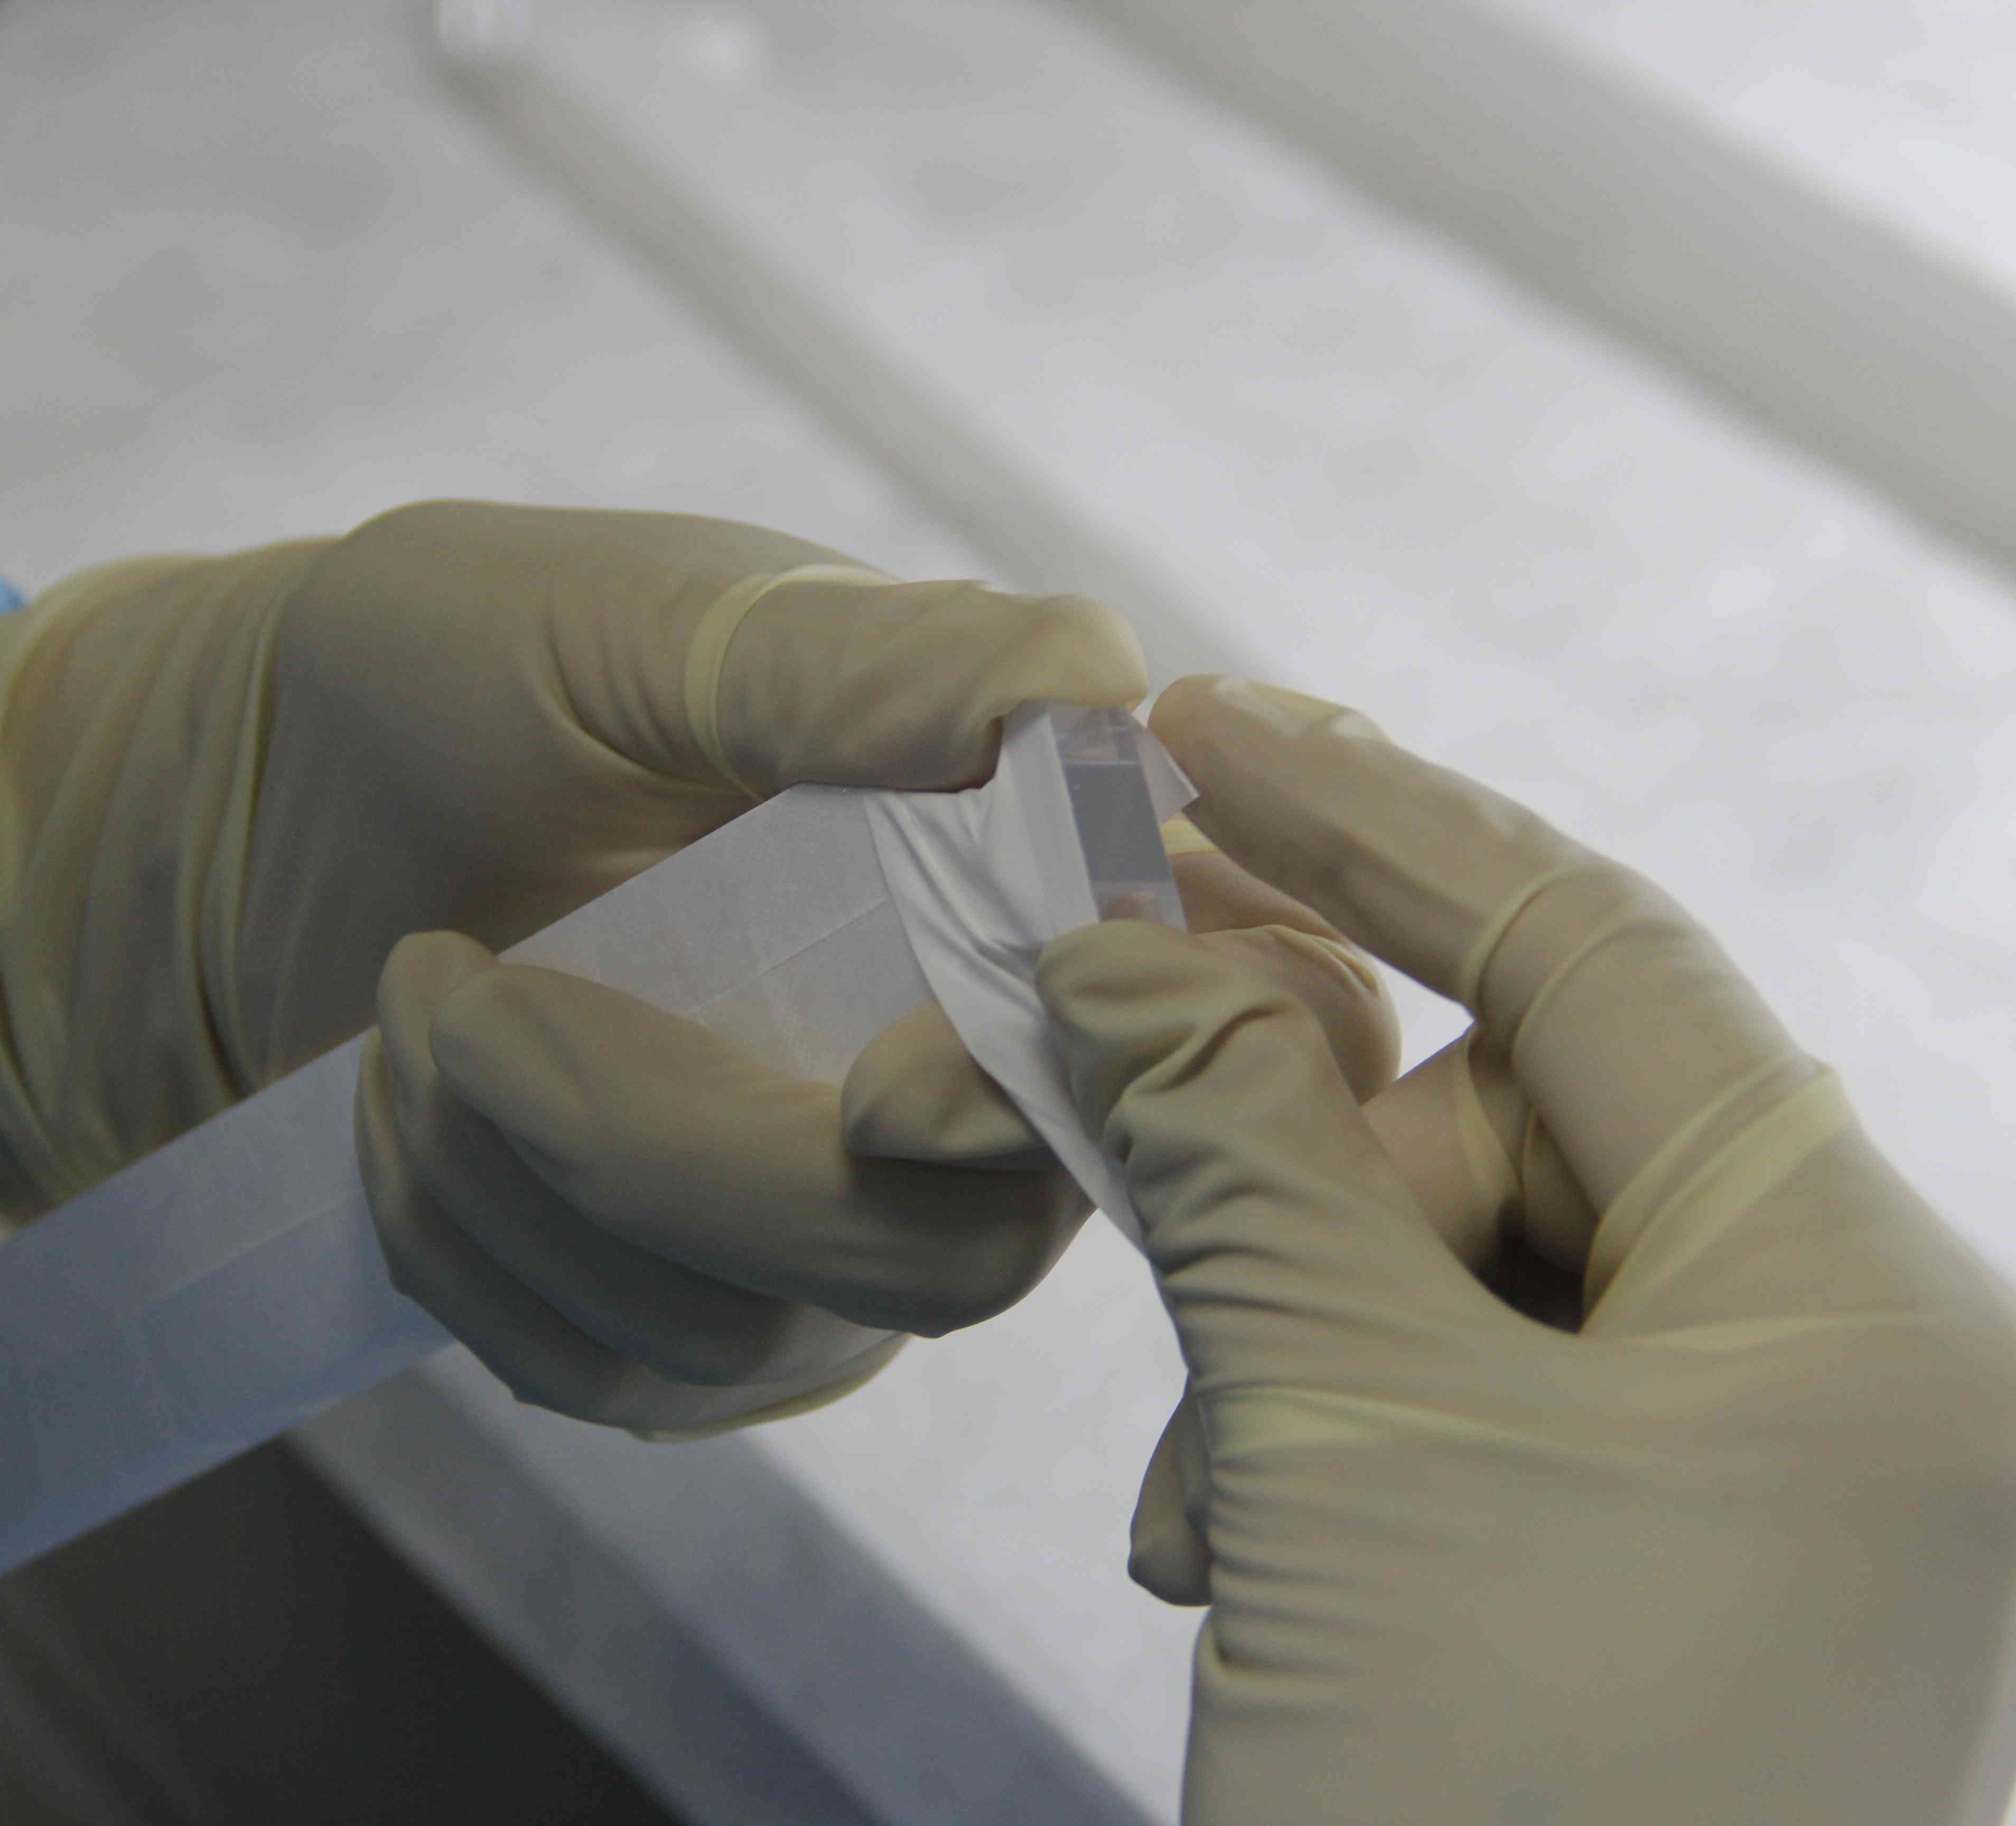
\includegraphics[width=0.25\textwidth]{chap/construction/fig/wrapping_b.jpg}
}
\subfloat[][]{
	\label{fig:construction:bar_wrapping_c}
	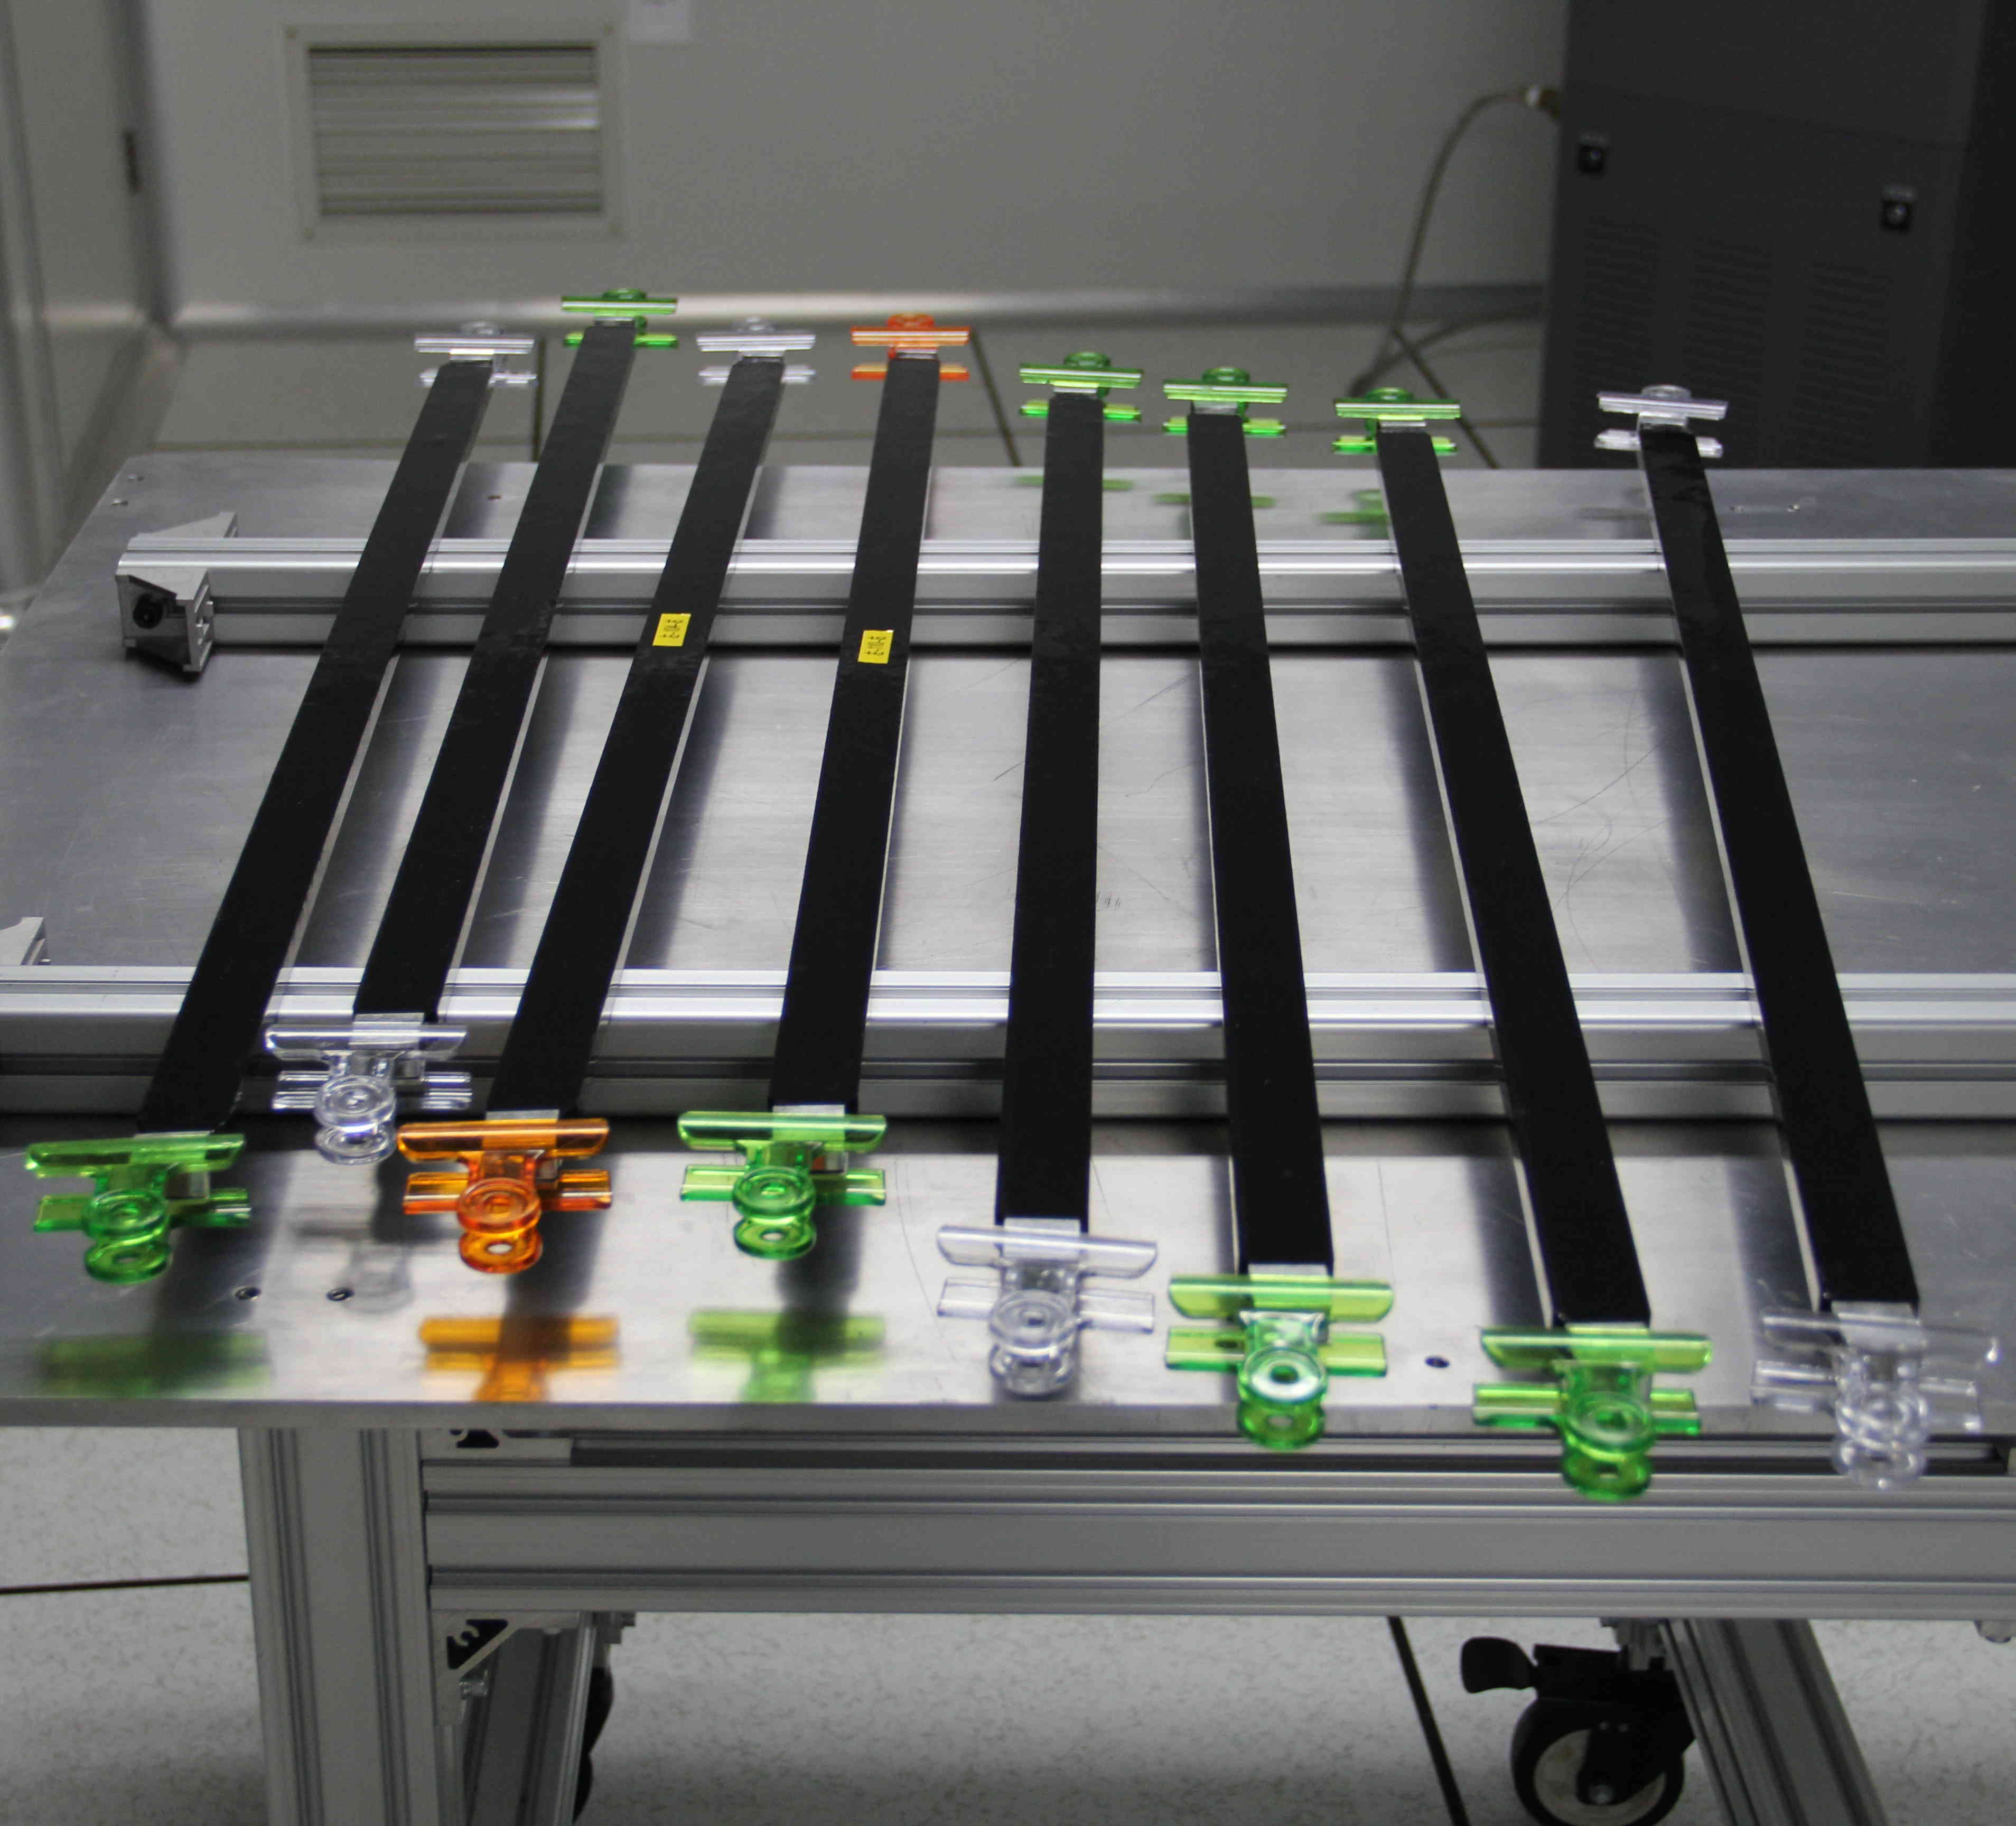
\includegraphics[width=0.25\textwidth]{chap/construction/fig/wrapping_c.jpg}
}
\subfloat[][]{
	\label{fig:construction:bar_wrapping_d}
	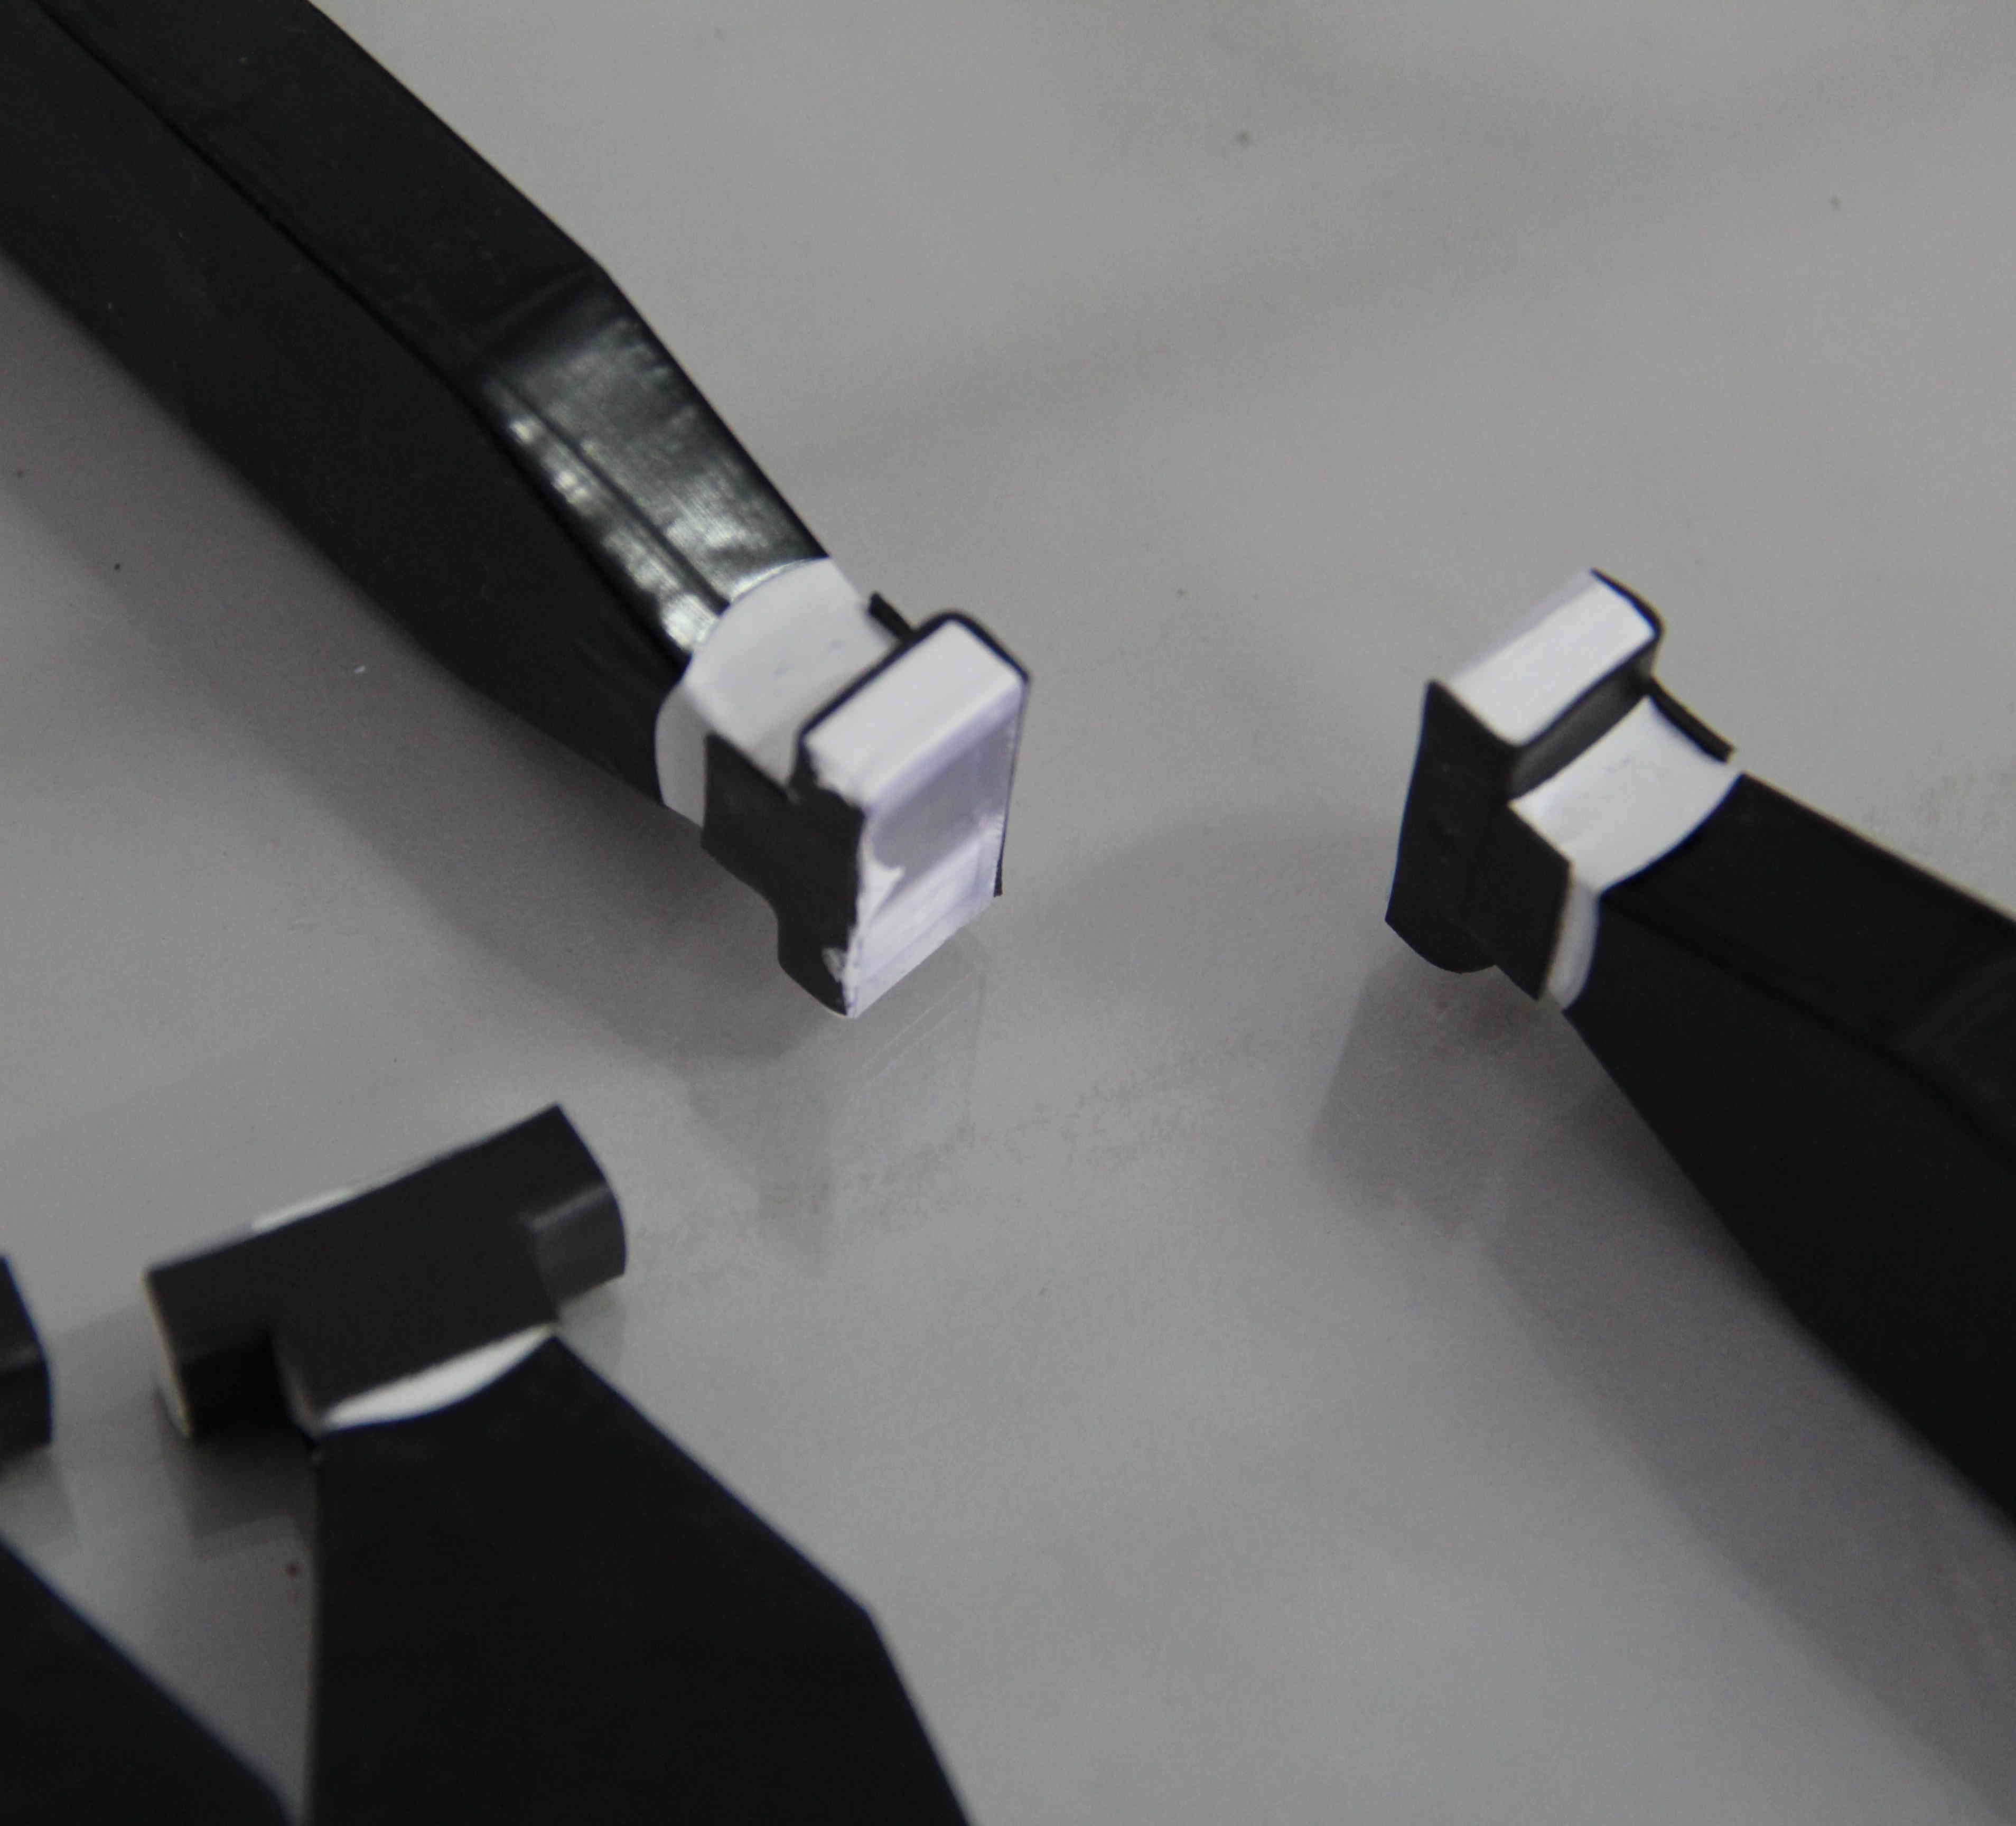
\includegraphics[width=0.25\textwidth]{chap/construction/fig/wrapping_d.jpg}
}
\caption{塑闪单元条的包装步骤}
\label{fig:construction:bar_wrapping}
\end{figure}
由于PSD的塑闪单元条端头采用了特殊的“工”字形设计(详见\ref{sec:description:psd_composition}节),因此端头的包装工艺与单元条主体并不一样:单元条主体内层包裹Tyvek纸,外层包裹黑色热缩管避光;单元条端头内层缠绕Teflon胶带,外层包裹黑色胶带避光。
具体的包装步骤如图\ref{fig:construction:bar_wrapping}所示,其中:a)使用Tyvek纸包裹单元条主体;b)使用Teflon包裹单元条端头;c)使用黑热缩管包裹单元条主体;d)使用黑色胶带包裹单元条端头。

最后,我们对包装后的塑闪单元条组件进行了宇宙线性能测试。
测试使用专门搭建的塑闪单元条批量测试平台(见图\ref{fig:construction:bar_testbench}),关于该平台以及此次测试的具体内容和结果在文献\parencite{bar_test_2015}中有详细的介绍,这里只做简单介绍。
\begin{figure}[htb]
\centering
\subfloat[][宇宙线批量测试平台]{
	\label{fig:construction:bar_testbench}
	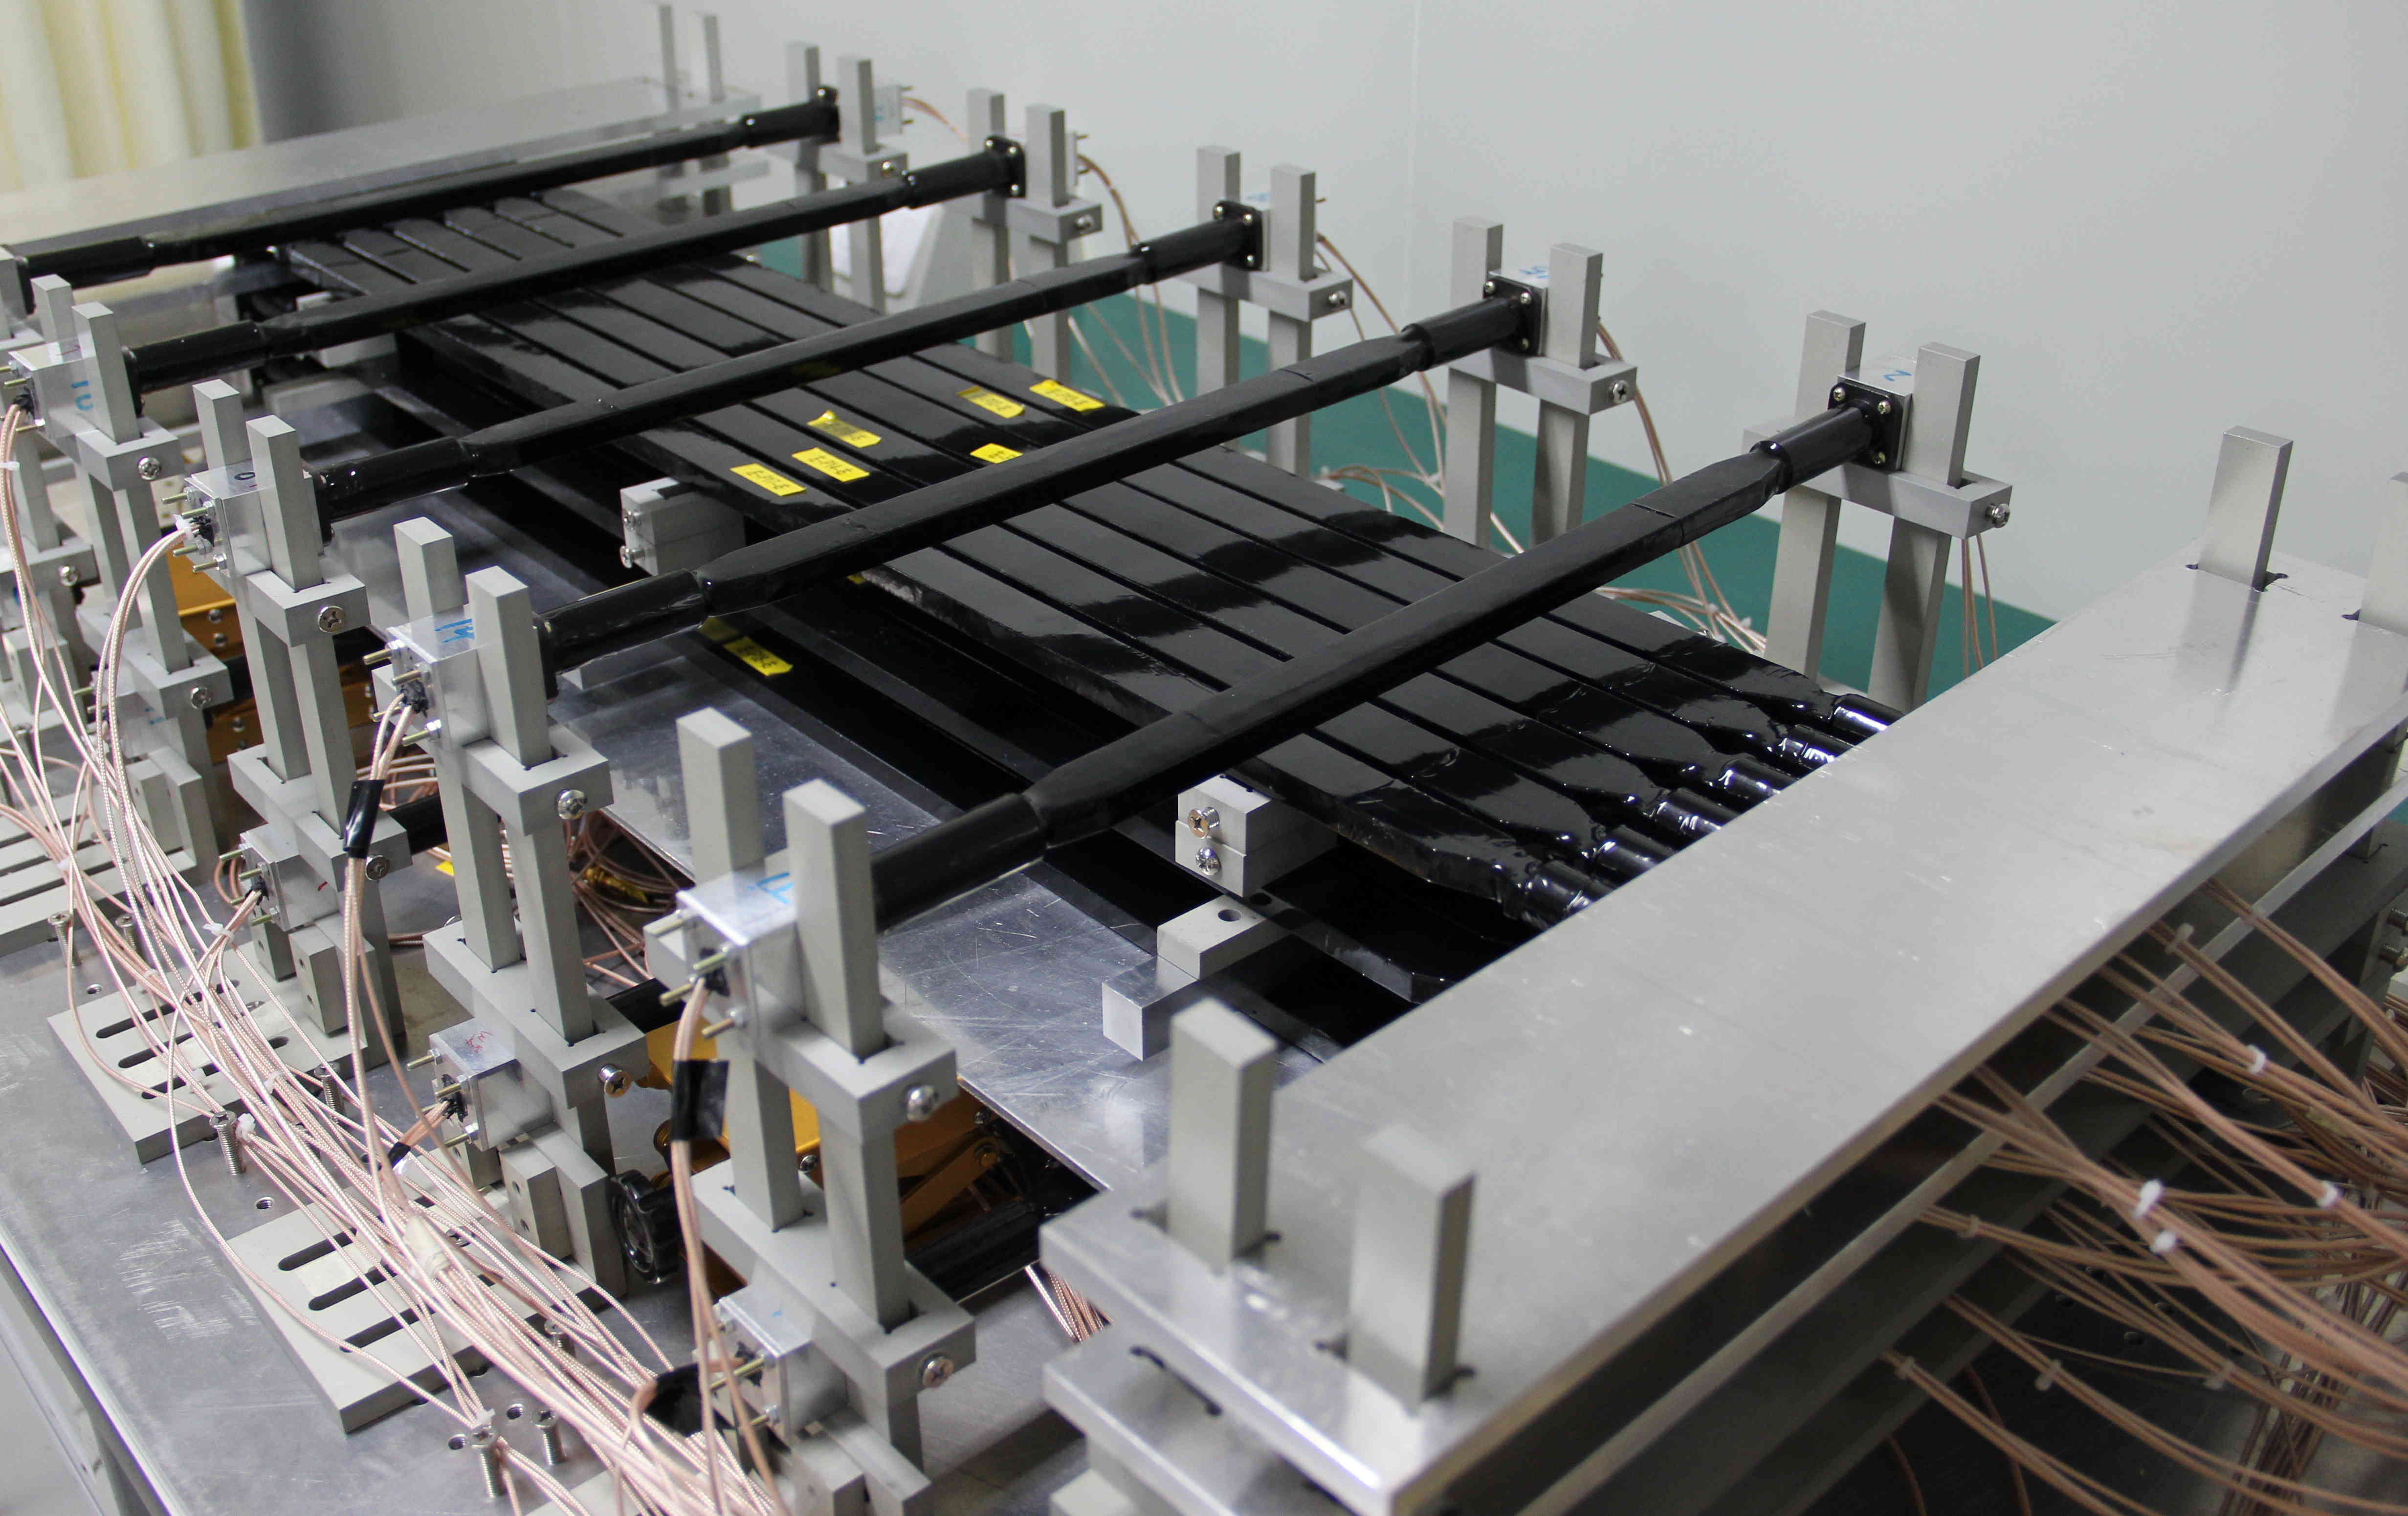
\includegraphics[width=0.48\textwidth]{chap/construction/fig/bar_cosmictest.jpg}
}
\subfloat[][测得的衰减长度分布(两端平均值,单位:cm)]{
	\label{fig:construction:attenuation_dist}
	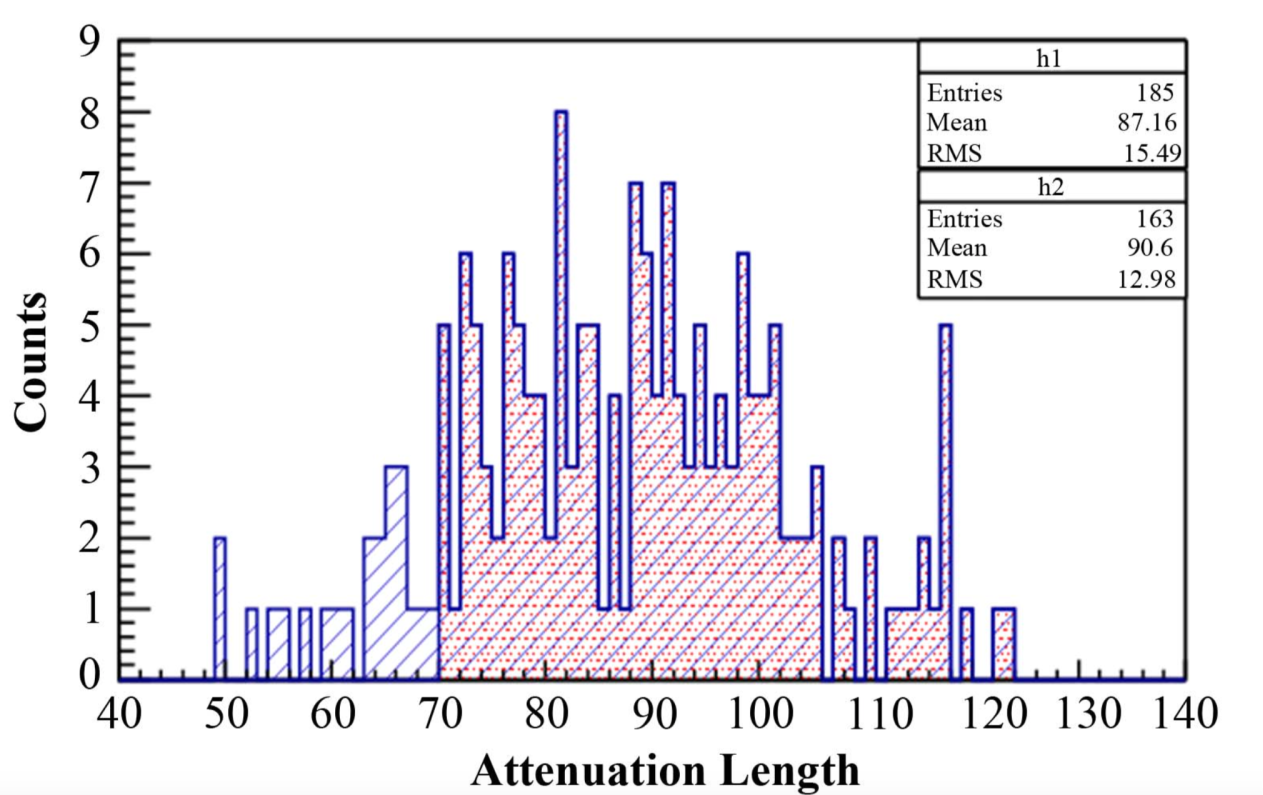
\includegraphics[width=0.48\textwidth]{chap/construction/fig/attenuation_dist.png}
}
\caption{塑闪单元条组件的宇宙线测试}
\label{fig:construction:bar_cosmictest}
\end{figure}
测试平台具有5个触发位置点,从而能够测量被测塑闪单元条在这5个位置点对垂直入射宇宙线的能量响应,即MIP响应。
这样就能得到每根单元条的衰减长度,我们一共测量了185根条子,它们的衰减长度分布如图\ref{fig:construction:attenuation_dist}所示。
由于测试平台使用的读出PMT具有相同的增益\parencite{bar_test_2015},因此通过对测试数据进一步分析和处理,我们还可以得到每根单元条的能量响应均匀性、相对光产额、能量分辨率以及探测效率等参数。
这些性能参数信息,加上之前得到的尺寸测量数据与热膨胀系数,将作为塑闪单元条组件筛选的重要依据(详见下一节)。

\subsection{塑闪单元条组件的筛选}
\label{sec:construction:bar_selection}
我们一共对185根裸塑闪单元条进行了包装和测试,最终从中挑选出了91根用于PSD的正式安装,其中包括2根B型单元条备份和7根A型单元条备份。
综合塑闪单元条的测试结果,我们把筛选判据归纳为以下几点:
\begin{enumerate}
	\item 单元条外观没有损伤,晶体内部清澈无杂散点,外部尺寸在设计公差内。
	\item 热膨胀系数在$\SI{7.8e-5}{}\sim \SI{8.8e-5}{\per\celsius}$范围内。热膨胀系数的定义为每摄氏度温度变化下塑闪单元条长度的相对变化率。
	\item 衰减曲线单调平滑,且两端得到的衰减长度都大于\SI{75}{cm}。
	\item 中间位置的相对光产额大于580道。假设在某测量位置点,单元条左右两端得到的MIP响应中心值分别为$MPV_L$和$MPV_R$,则它们的几何平均值$\sqrt{MPV_L \cdot MPV_R}$与该单元条的光产额大小相关。由于测试平台使用的读出PMT工作在相同的增益下\parencite{bar_test_2015},可以使用原始ADC道数计算该值并直接用来比较,因此我们把也把该数值称为相对光产额。PSD正式使用的单元条光产额越大越好,根据测试数据的实际分布,我们要求中心位置处得到的相对光产额数值大于580道。
	\item 光产额均匀性好于\SI{5}{\percent}。在理想情况下,塑闪单元体的光衰减服从指数衰减规律,此时不同位置得到的相对光产额应该是相等的。实际中,PSD的相对光产额中间位置小,两端高。我们计算不同测量位置得到的相对光产额相对于中间位置处的相对差异,并使用其最大值代表该单元条光产额的均匀性。我们要求PSD正式使用的光产额均匀性要好于\SI{5}{\percent}。
	\item 中间位置处的MIP响应能量分辨率好于\SI{25}{\percent},这是PSD的设计要求。
	\item 探测效率大于\SI{95}{\percent},这也是PSD的设计要求。
\end{enumerate}

\section{PSD探测器的整体组装}
\label{sec:construction:psd_assembly}

结合PMT组件和塑闪单元条组件的筛选结果,我们对它们进行了配对,基本原则是衰减长度和相对光产额较大的单元条组件配对增益较小的PMT组件。
配对完成后,我们正式开始了PSD的整体装配。

PSD的整体装配就是将各个功能模块和组件组装成一个功能完整的探测器。
PSD采用模块化设计,各个功能模块间的接口明确且耦合程度较低,因此PSD的整体装配过程层次清晰,便于质量控制和管理。
特别需要提出的一点是:PSD中PMT组件和塑闪单元条组件的安装是相互独立的,两个组件并不是耦合在一起后才安装到PSD支撑结构中,而是通过PMT组件的铝合金保护套固定在梁结构上后产生的推力将它们紧密按压在一起完成耦合。
完整的PSD总装步骤如图\ref{fig:construction:psd_assembly}所示,下面对每个步骤进行简单介绍:
\begin{figure}[htb]
\centering
\subfloat[][布置金属导电胶带]{
	\label{fig:construction:assembly_a}
	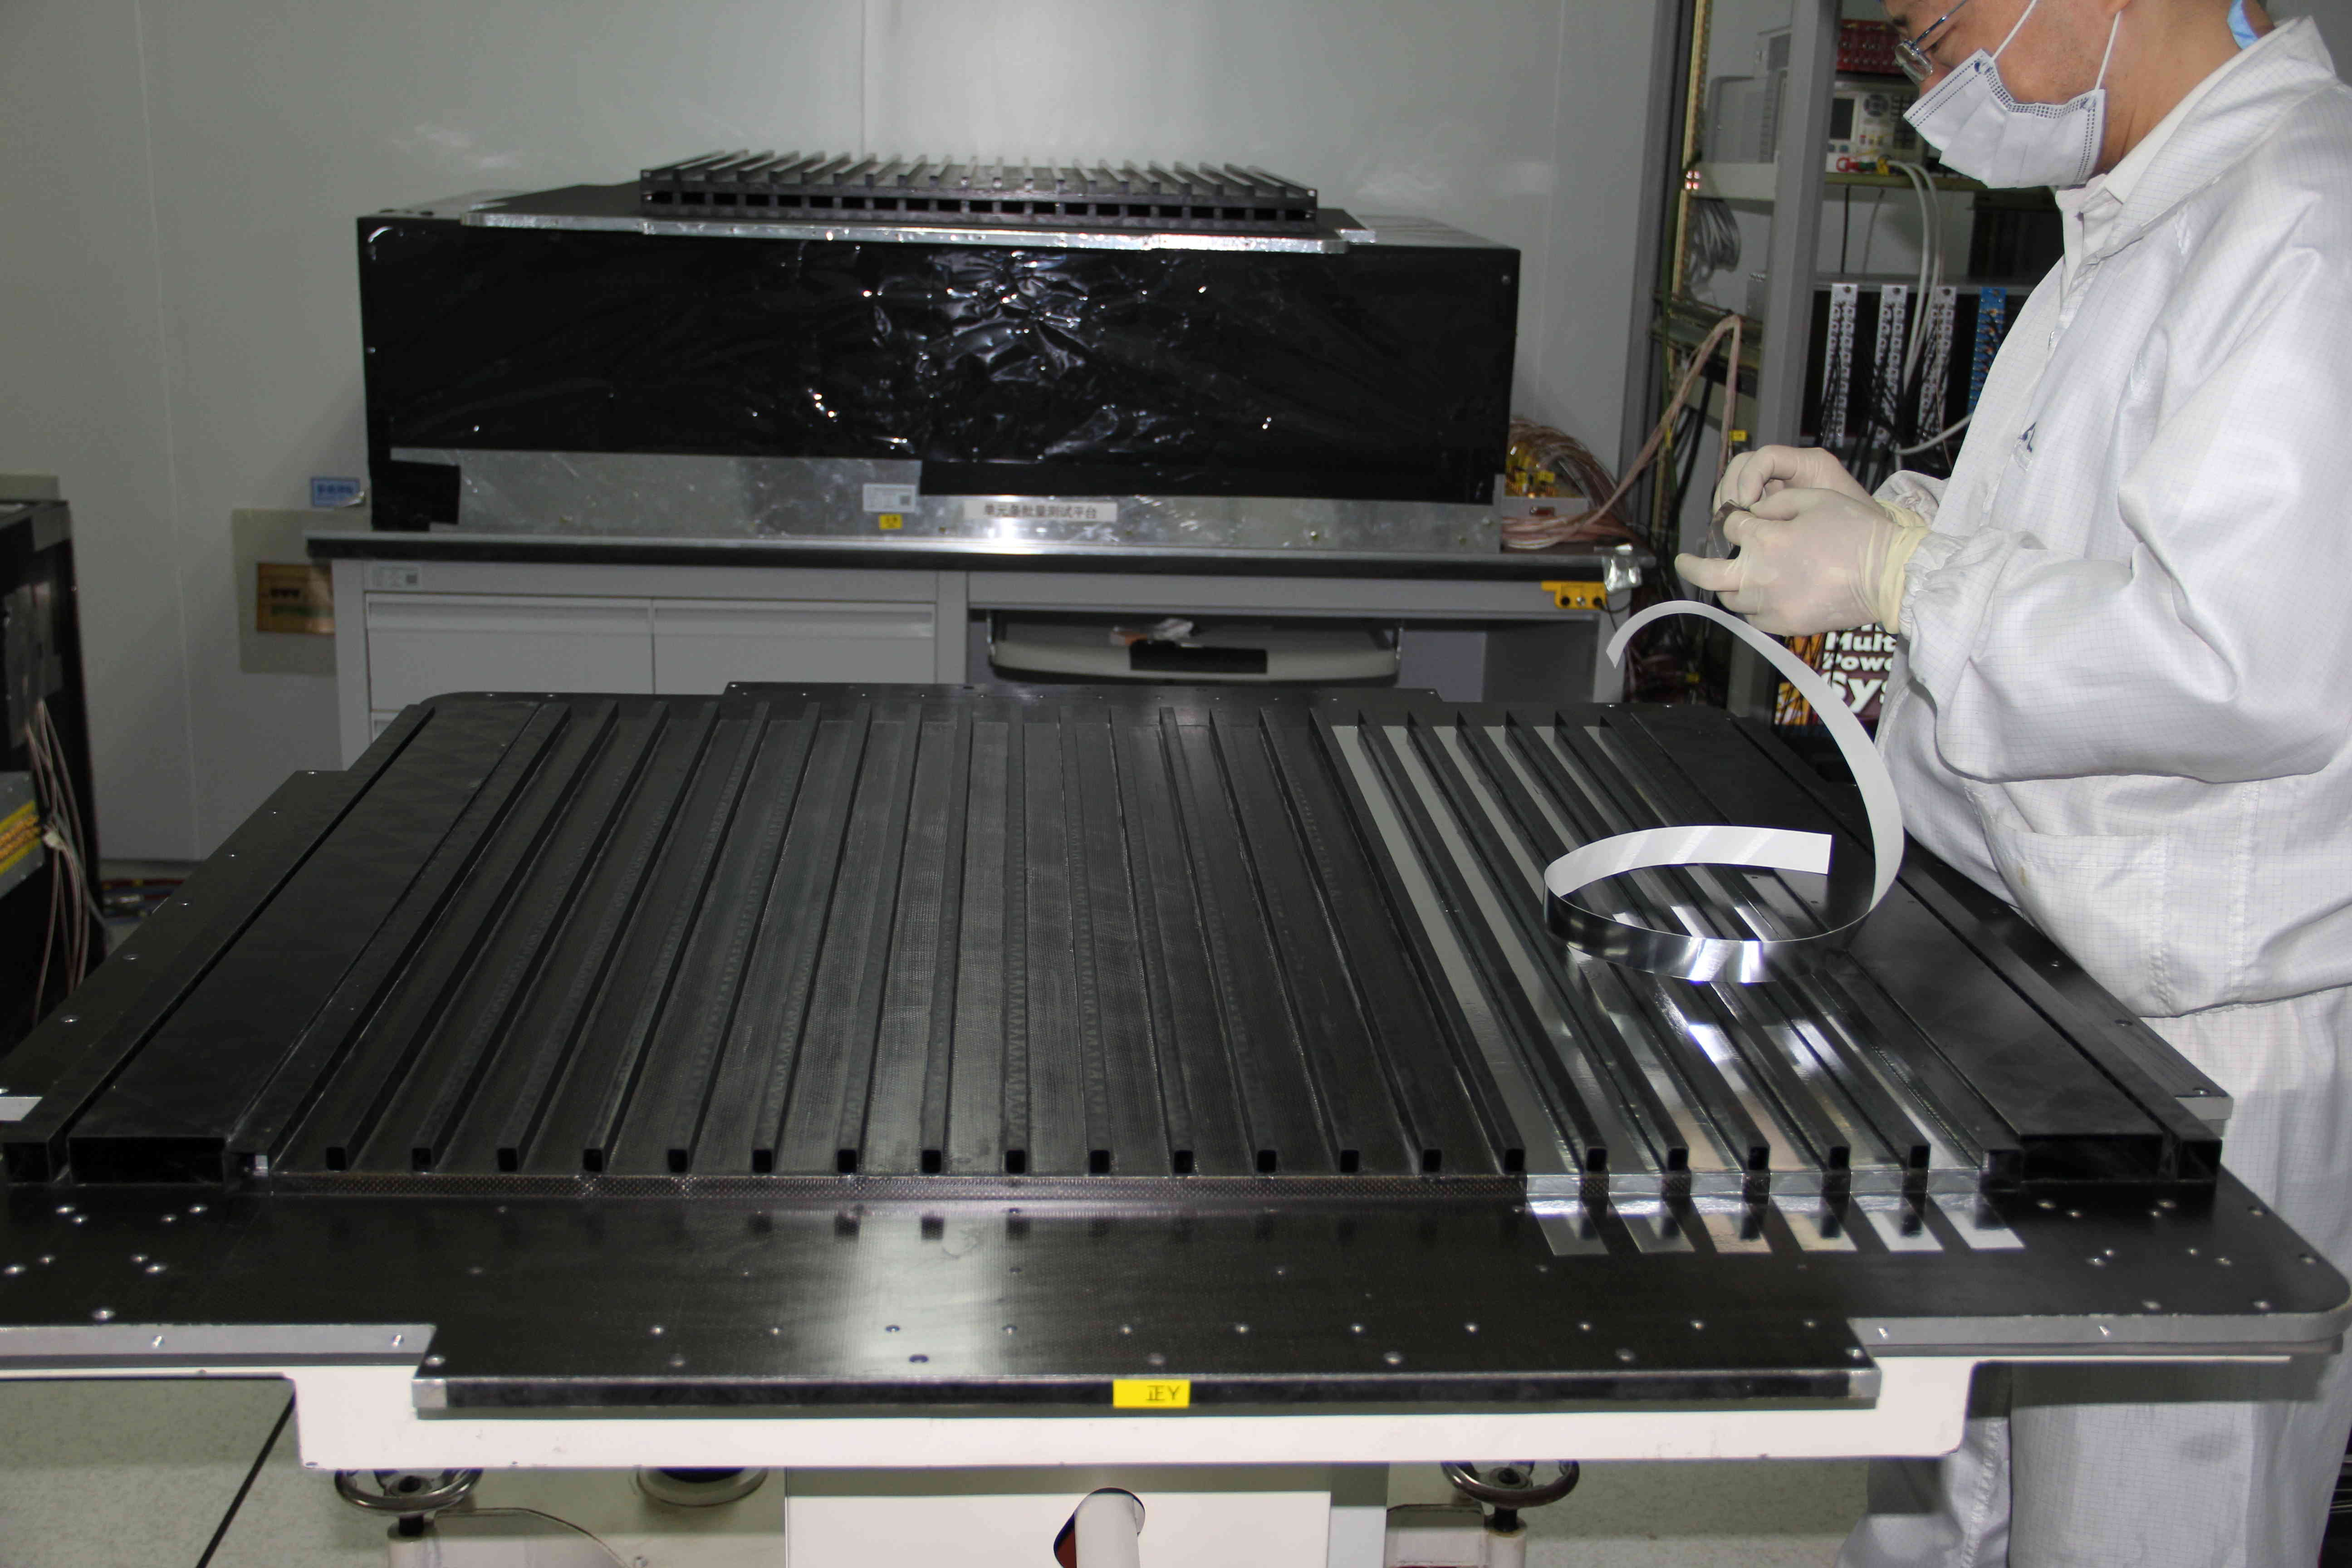
\includegraphics[width=0.33\textwidth]{chap/construction/fig/assembly_a.jpg}
}
\subfloat[][安装塑闪单元条组件]{
	\label{fig:construction:assembly_b}
	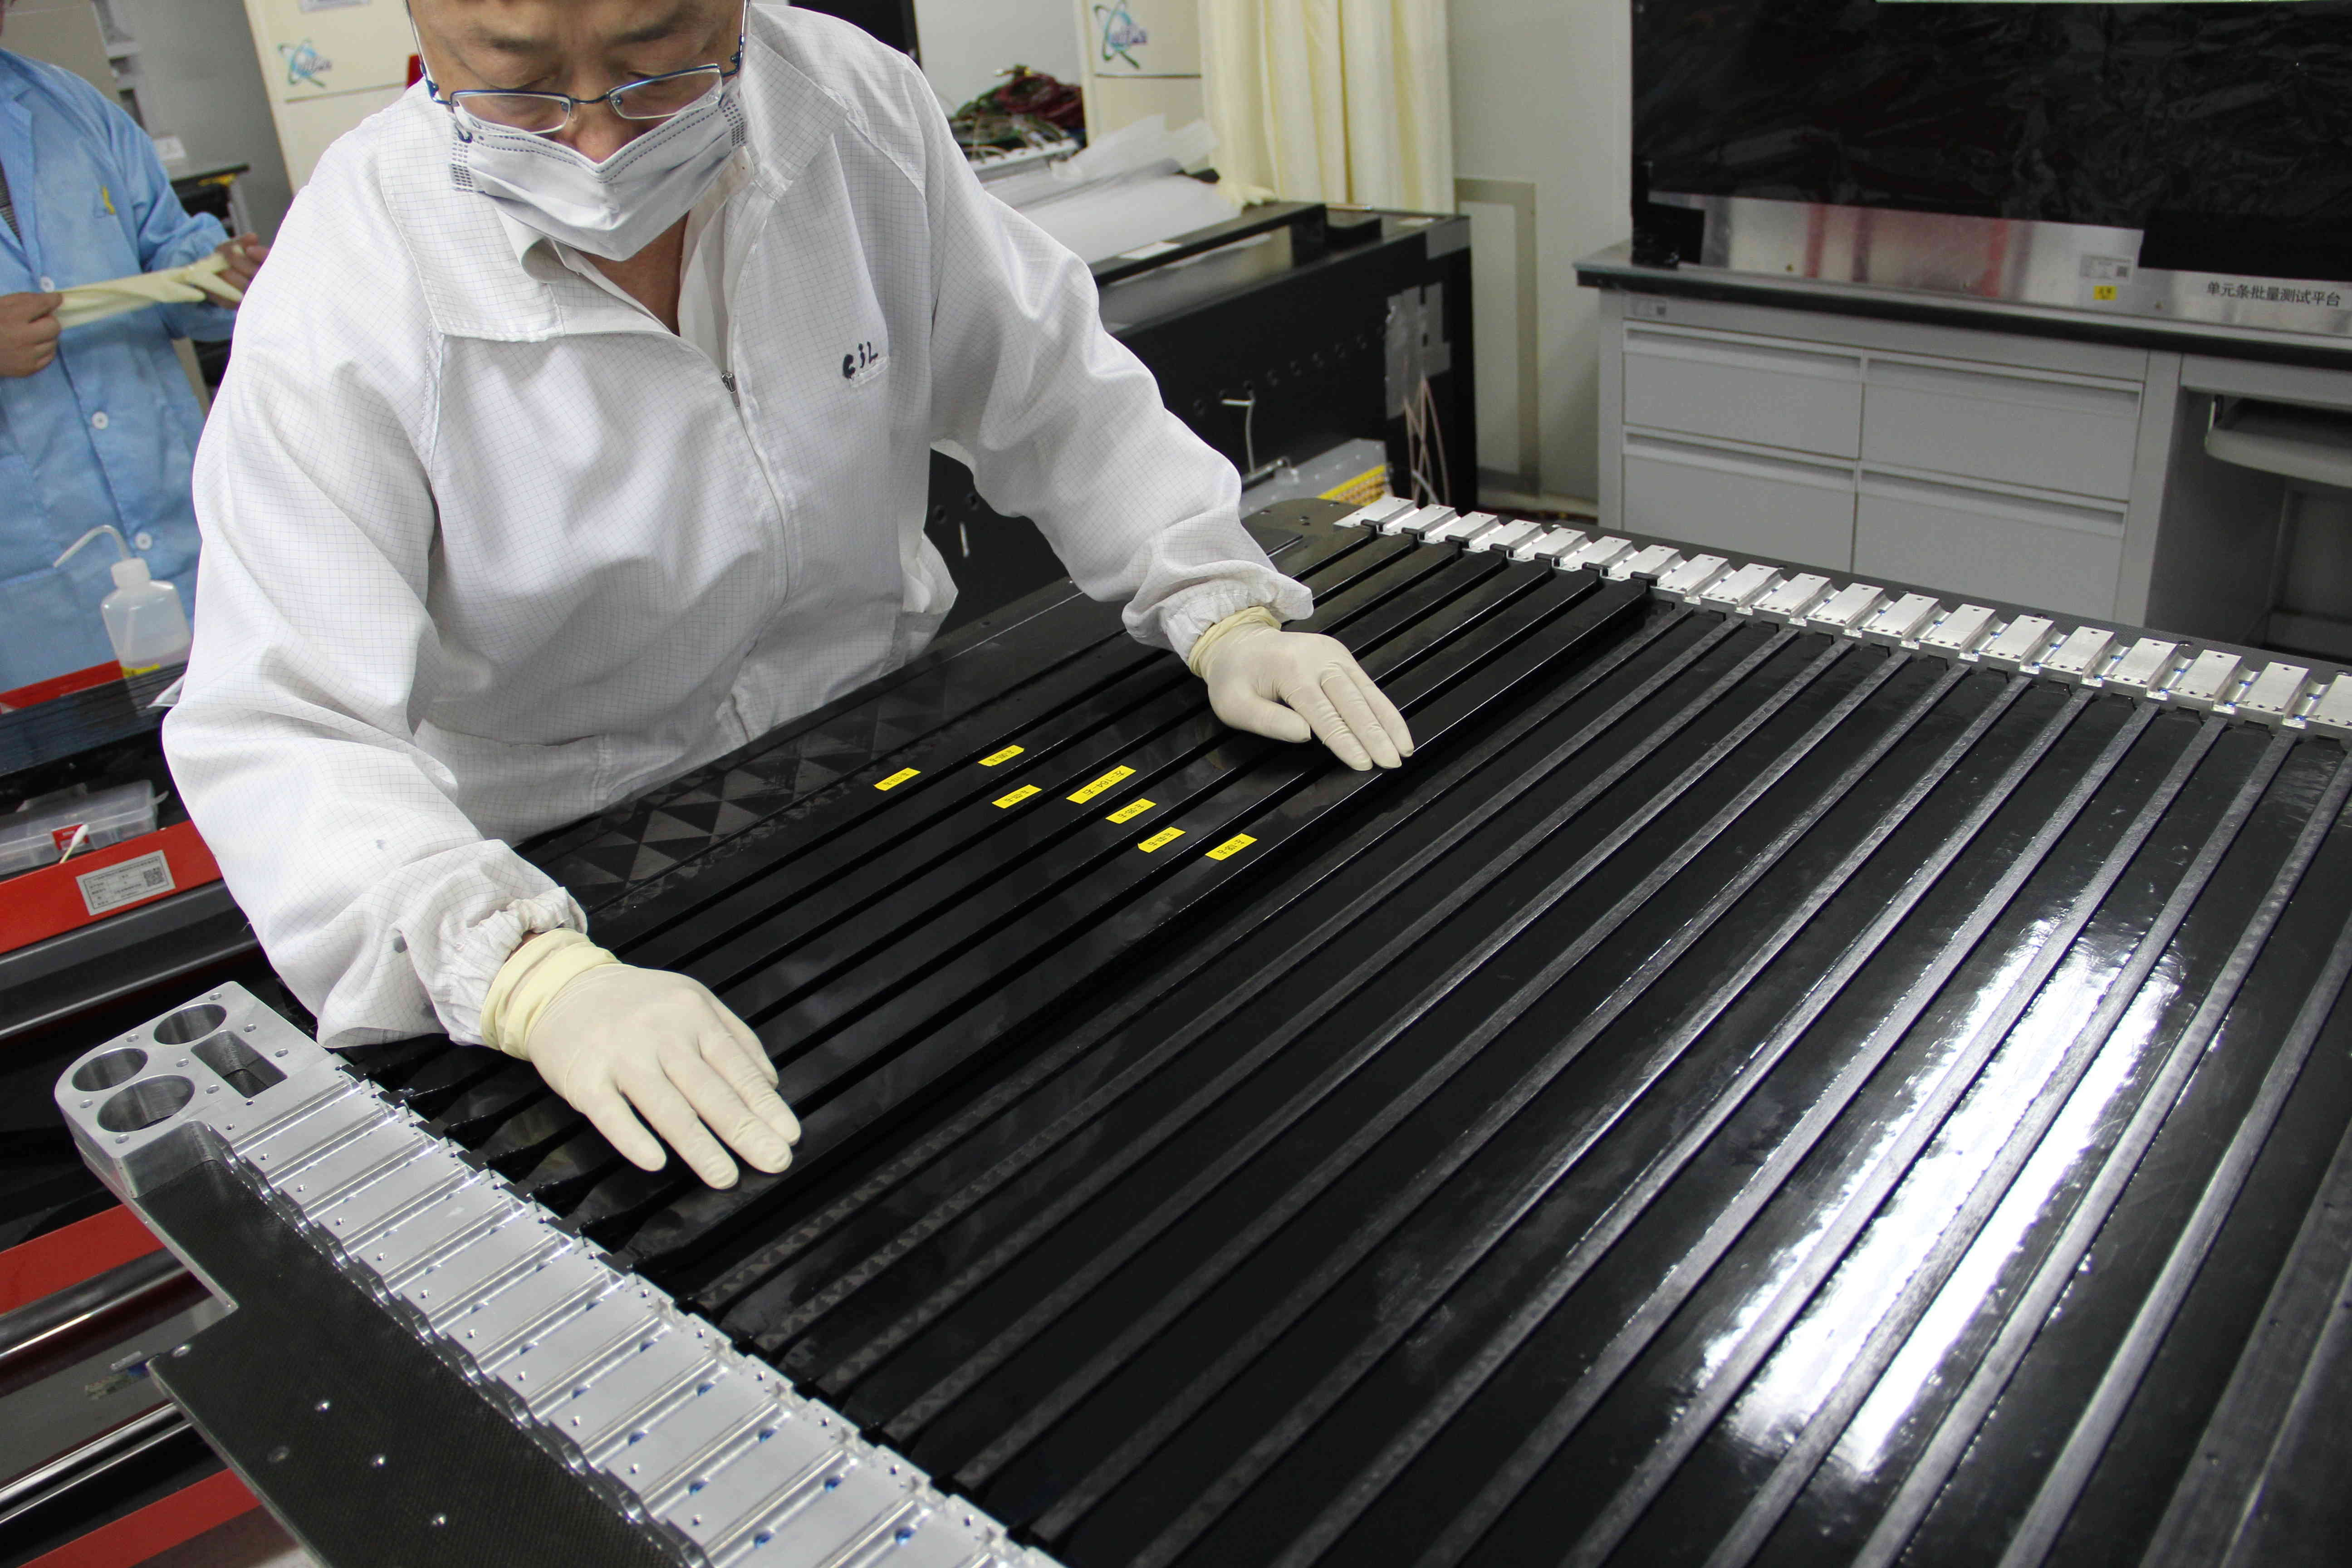
\includegraphics[width=0.33\textwidth]{chap/construction/fig/assembly_b.jpg}
}
\subfloat[][安装PMT组件]{
	\label{fig:construction:assembly_c}
	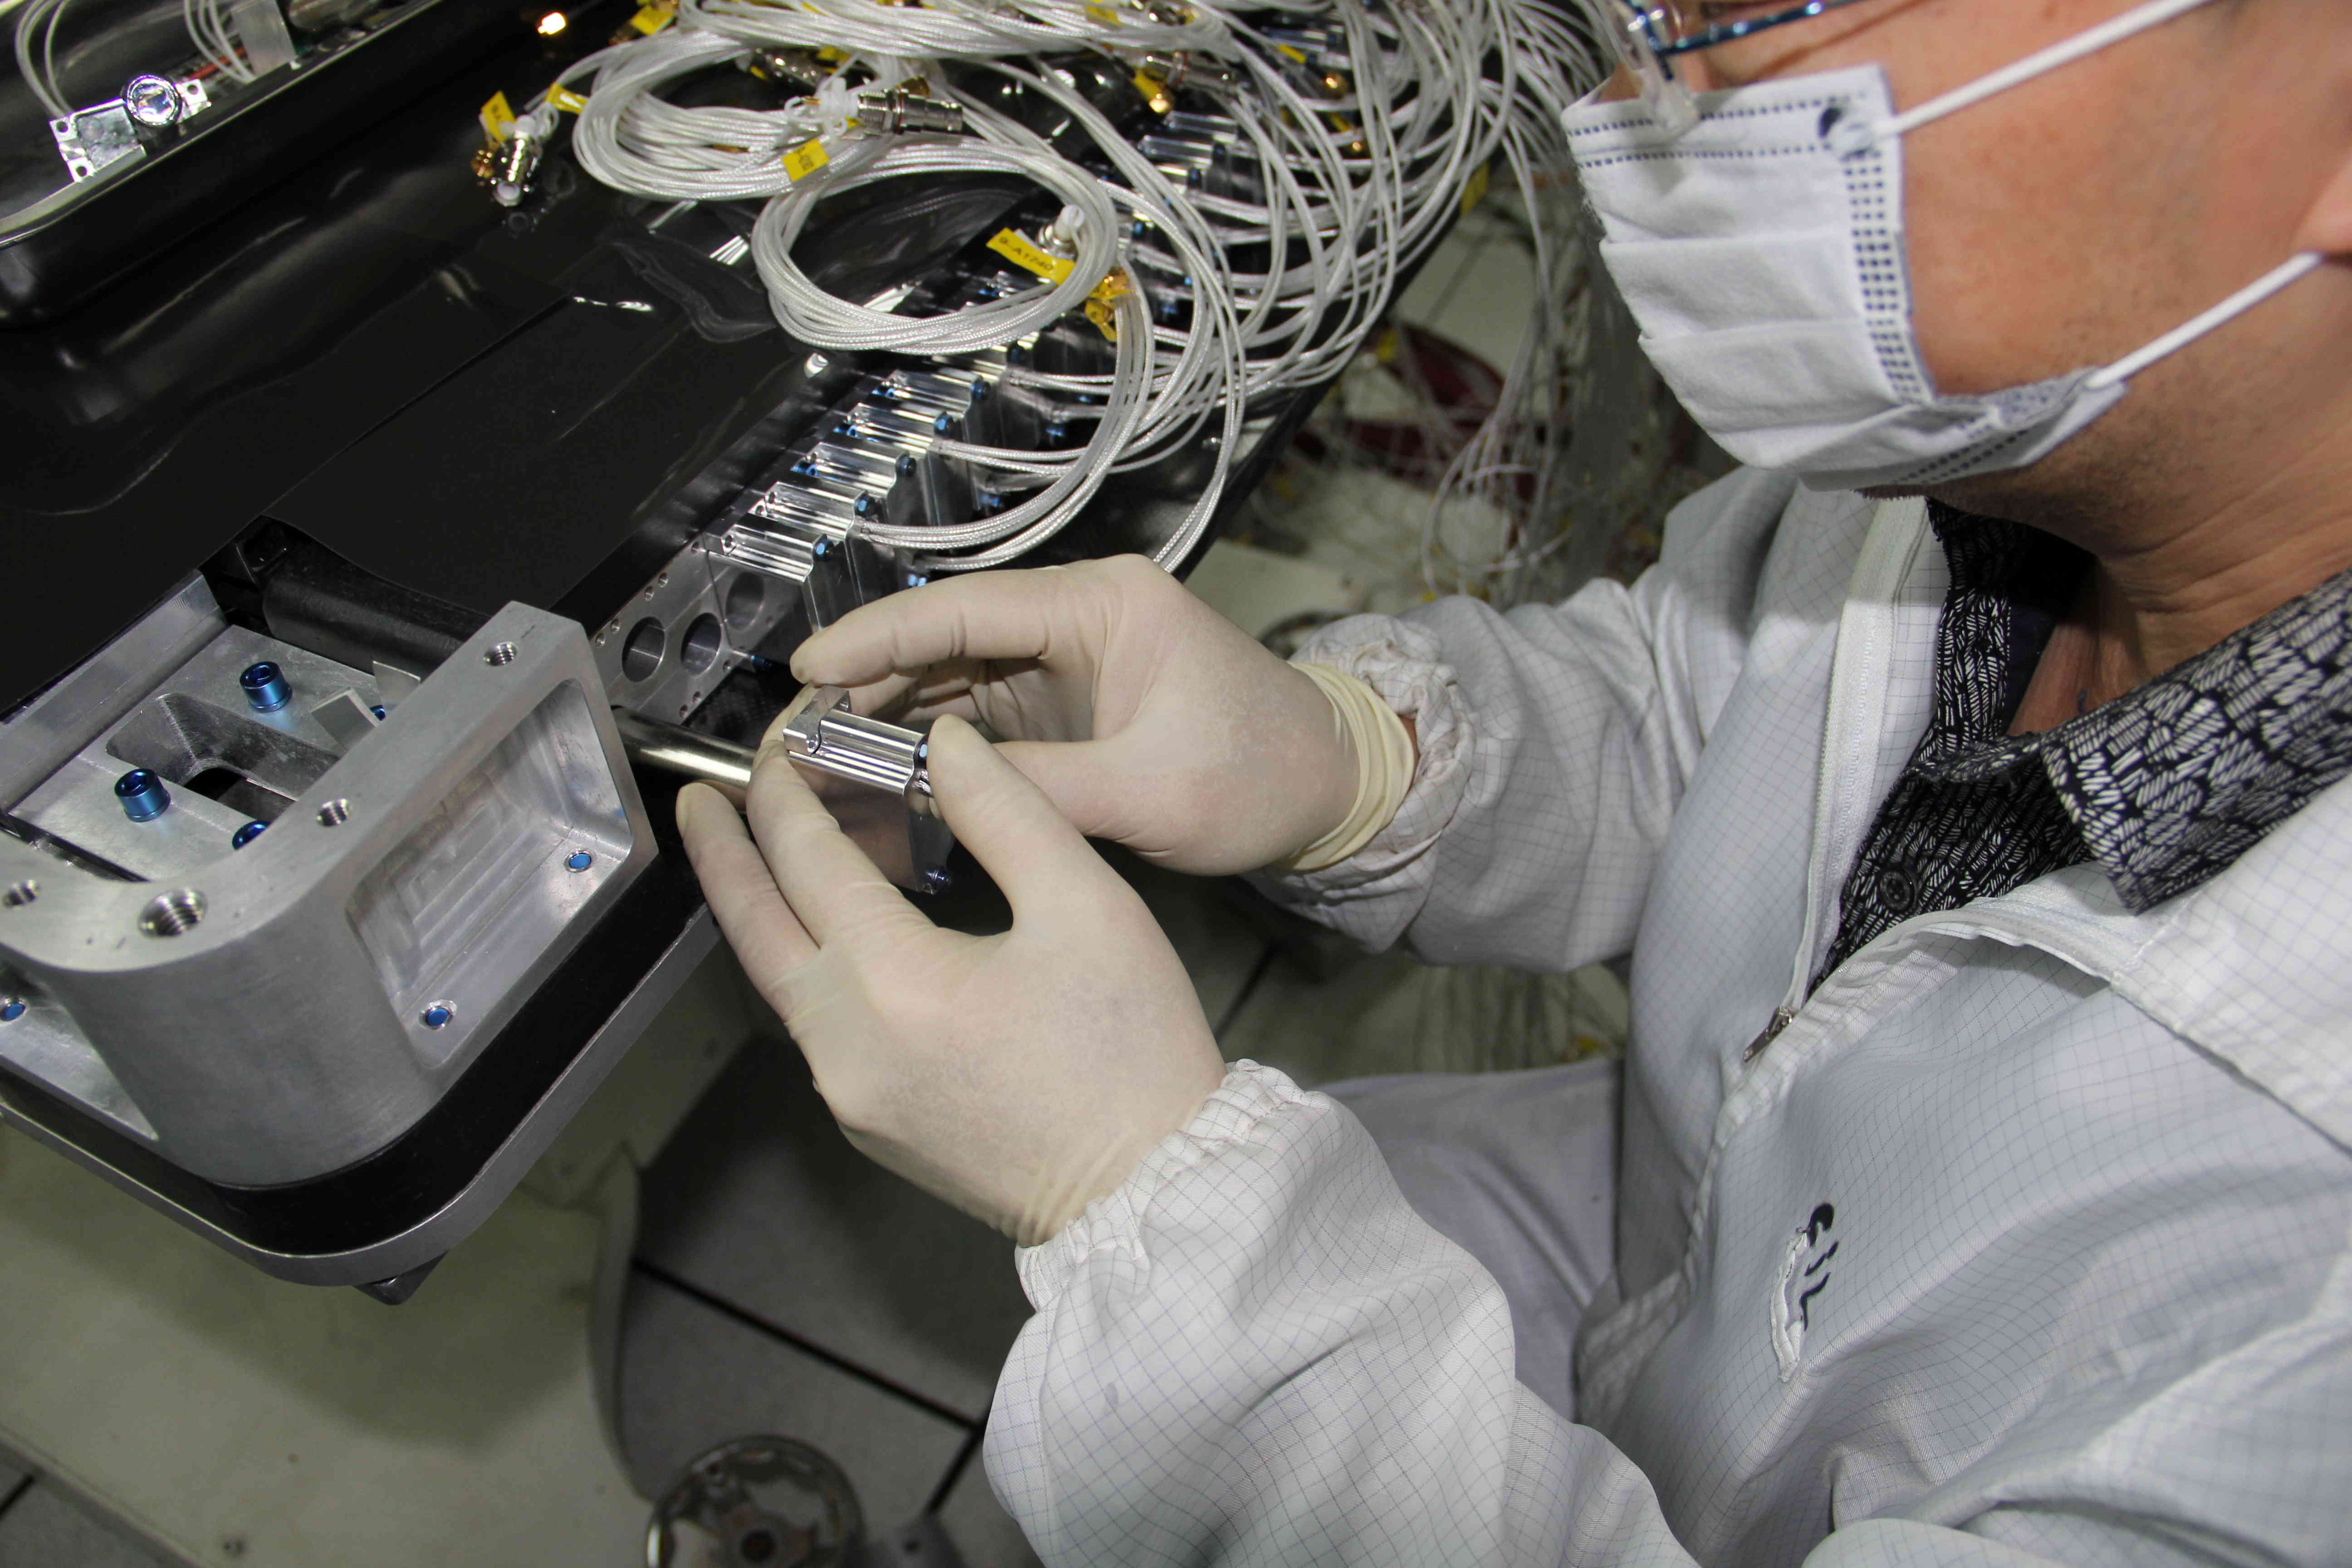
\includegraphics[width=0.33\textwidth]{chap/construction/fig/assembly_c.jpg}
}
//
\subfloat[][电装]{
	\label{fig:construction:assembly_d}
	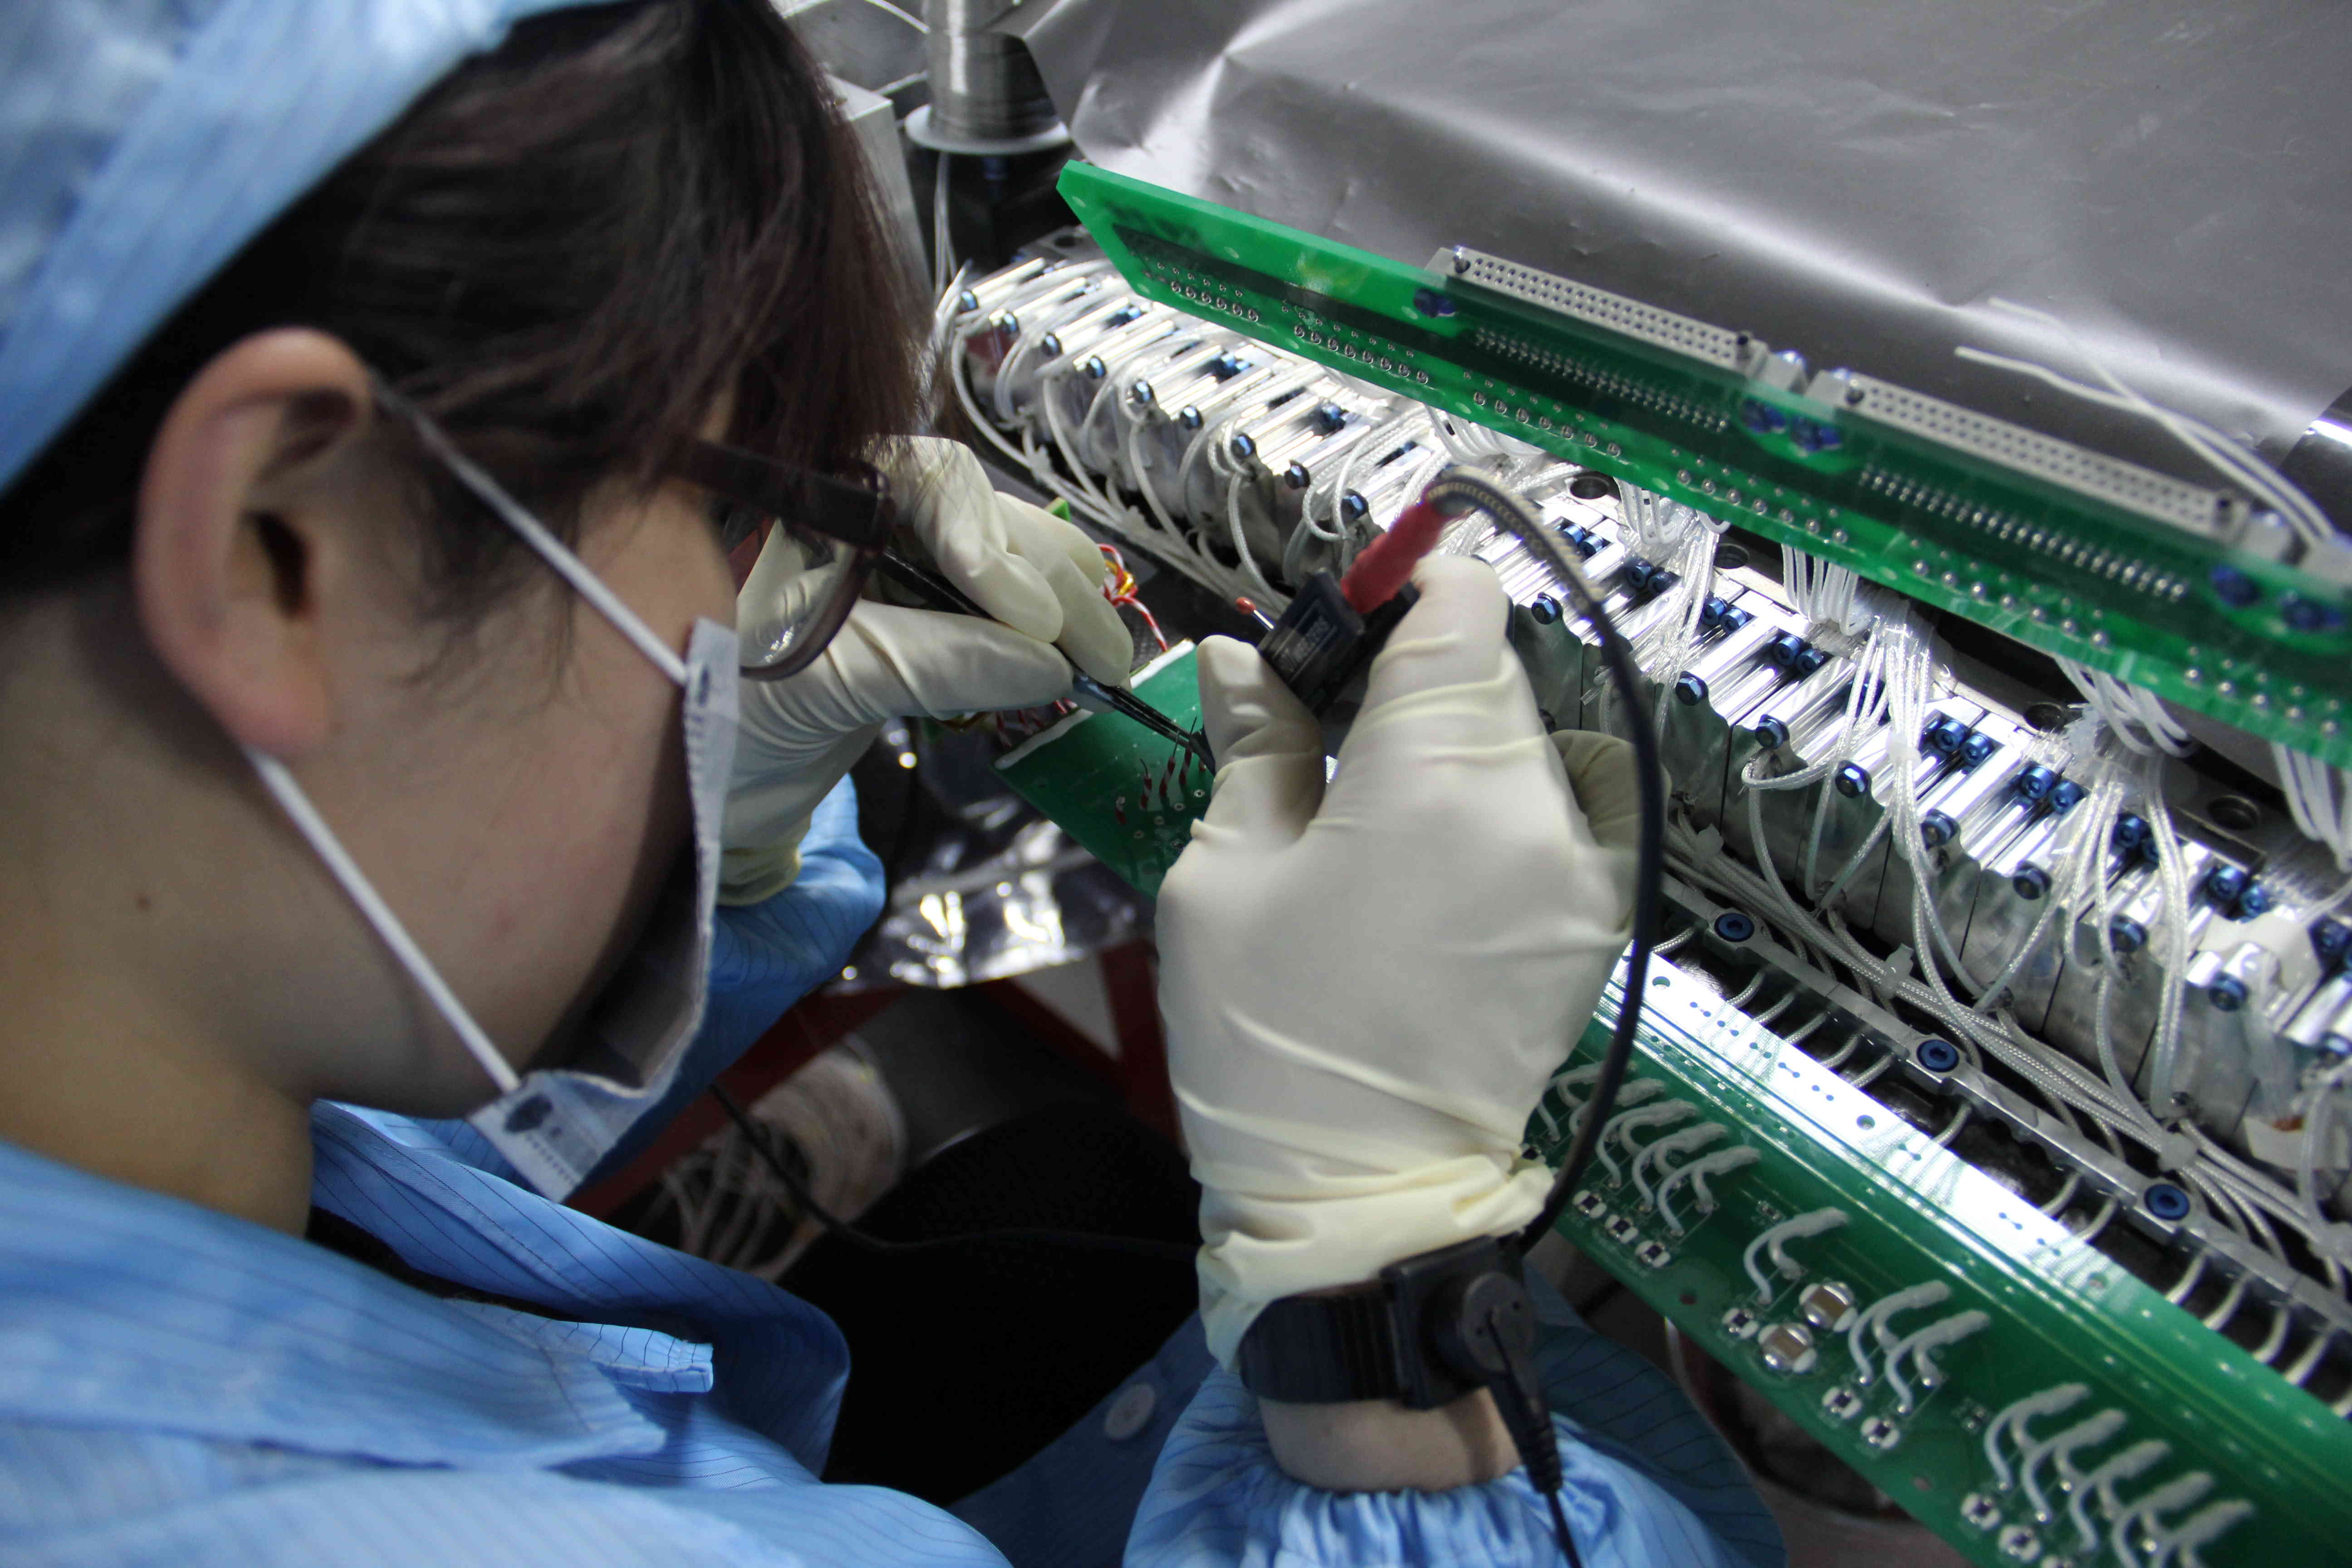
\includegraphics[width=0.33\textwidth]{chap/construction/fig/assembly_d.jpg}
}
\subfloat[][安装FEE机箱]{
	\label{fig:construction:assembly_e}
	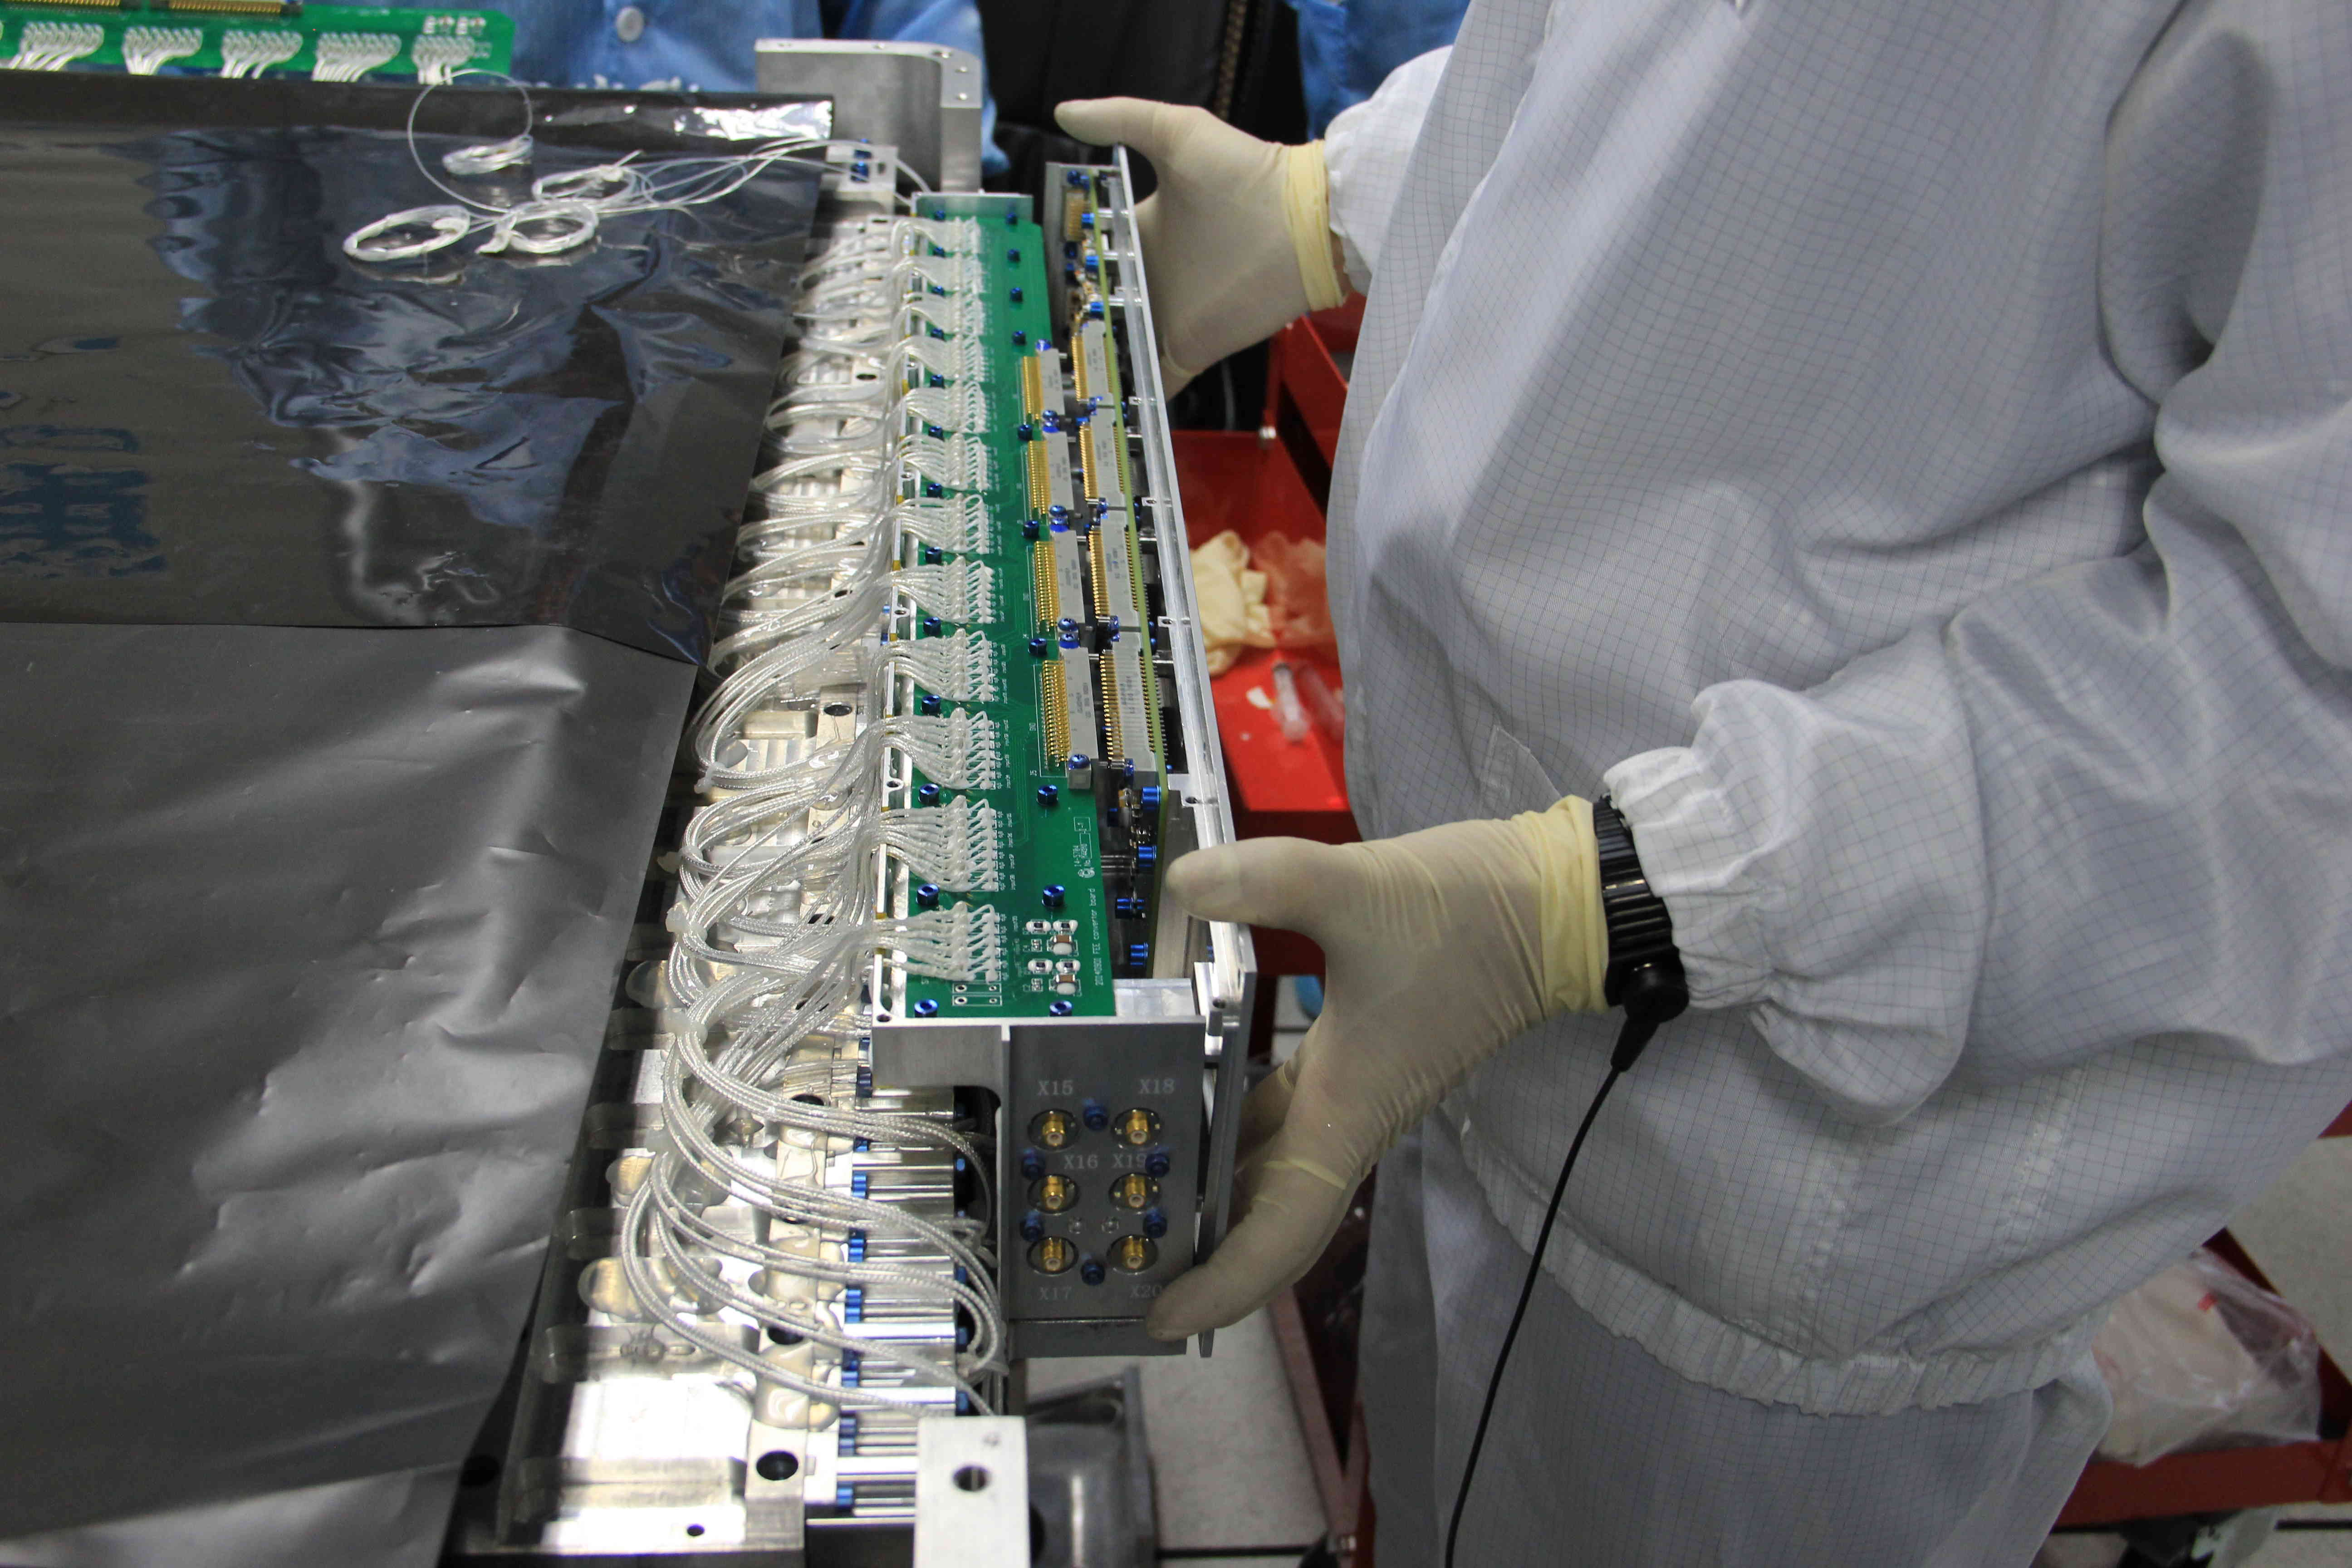
\includegraphics[width=0.33\textwidth]{chap/construction/fig/assembly_e.jpg}
}
\subfloat[][封顶]{
	\label{fig:construction:assembly_f}
	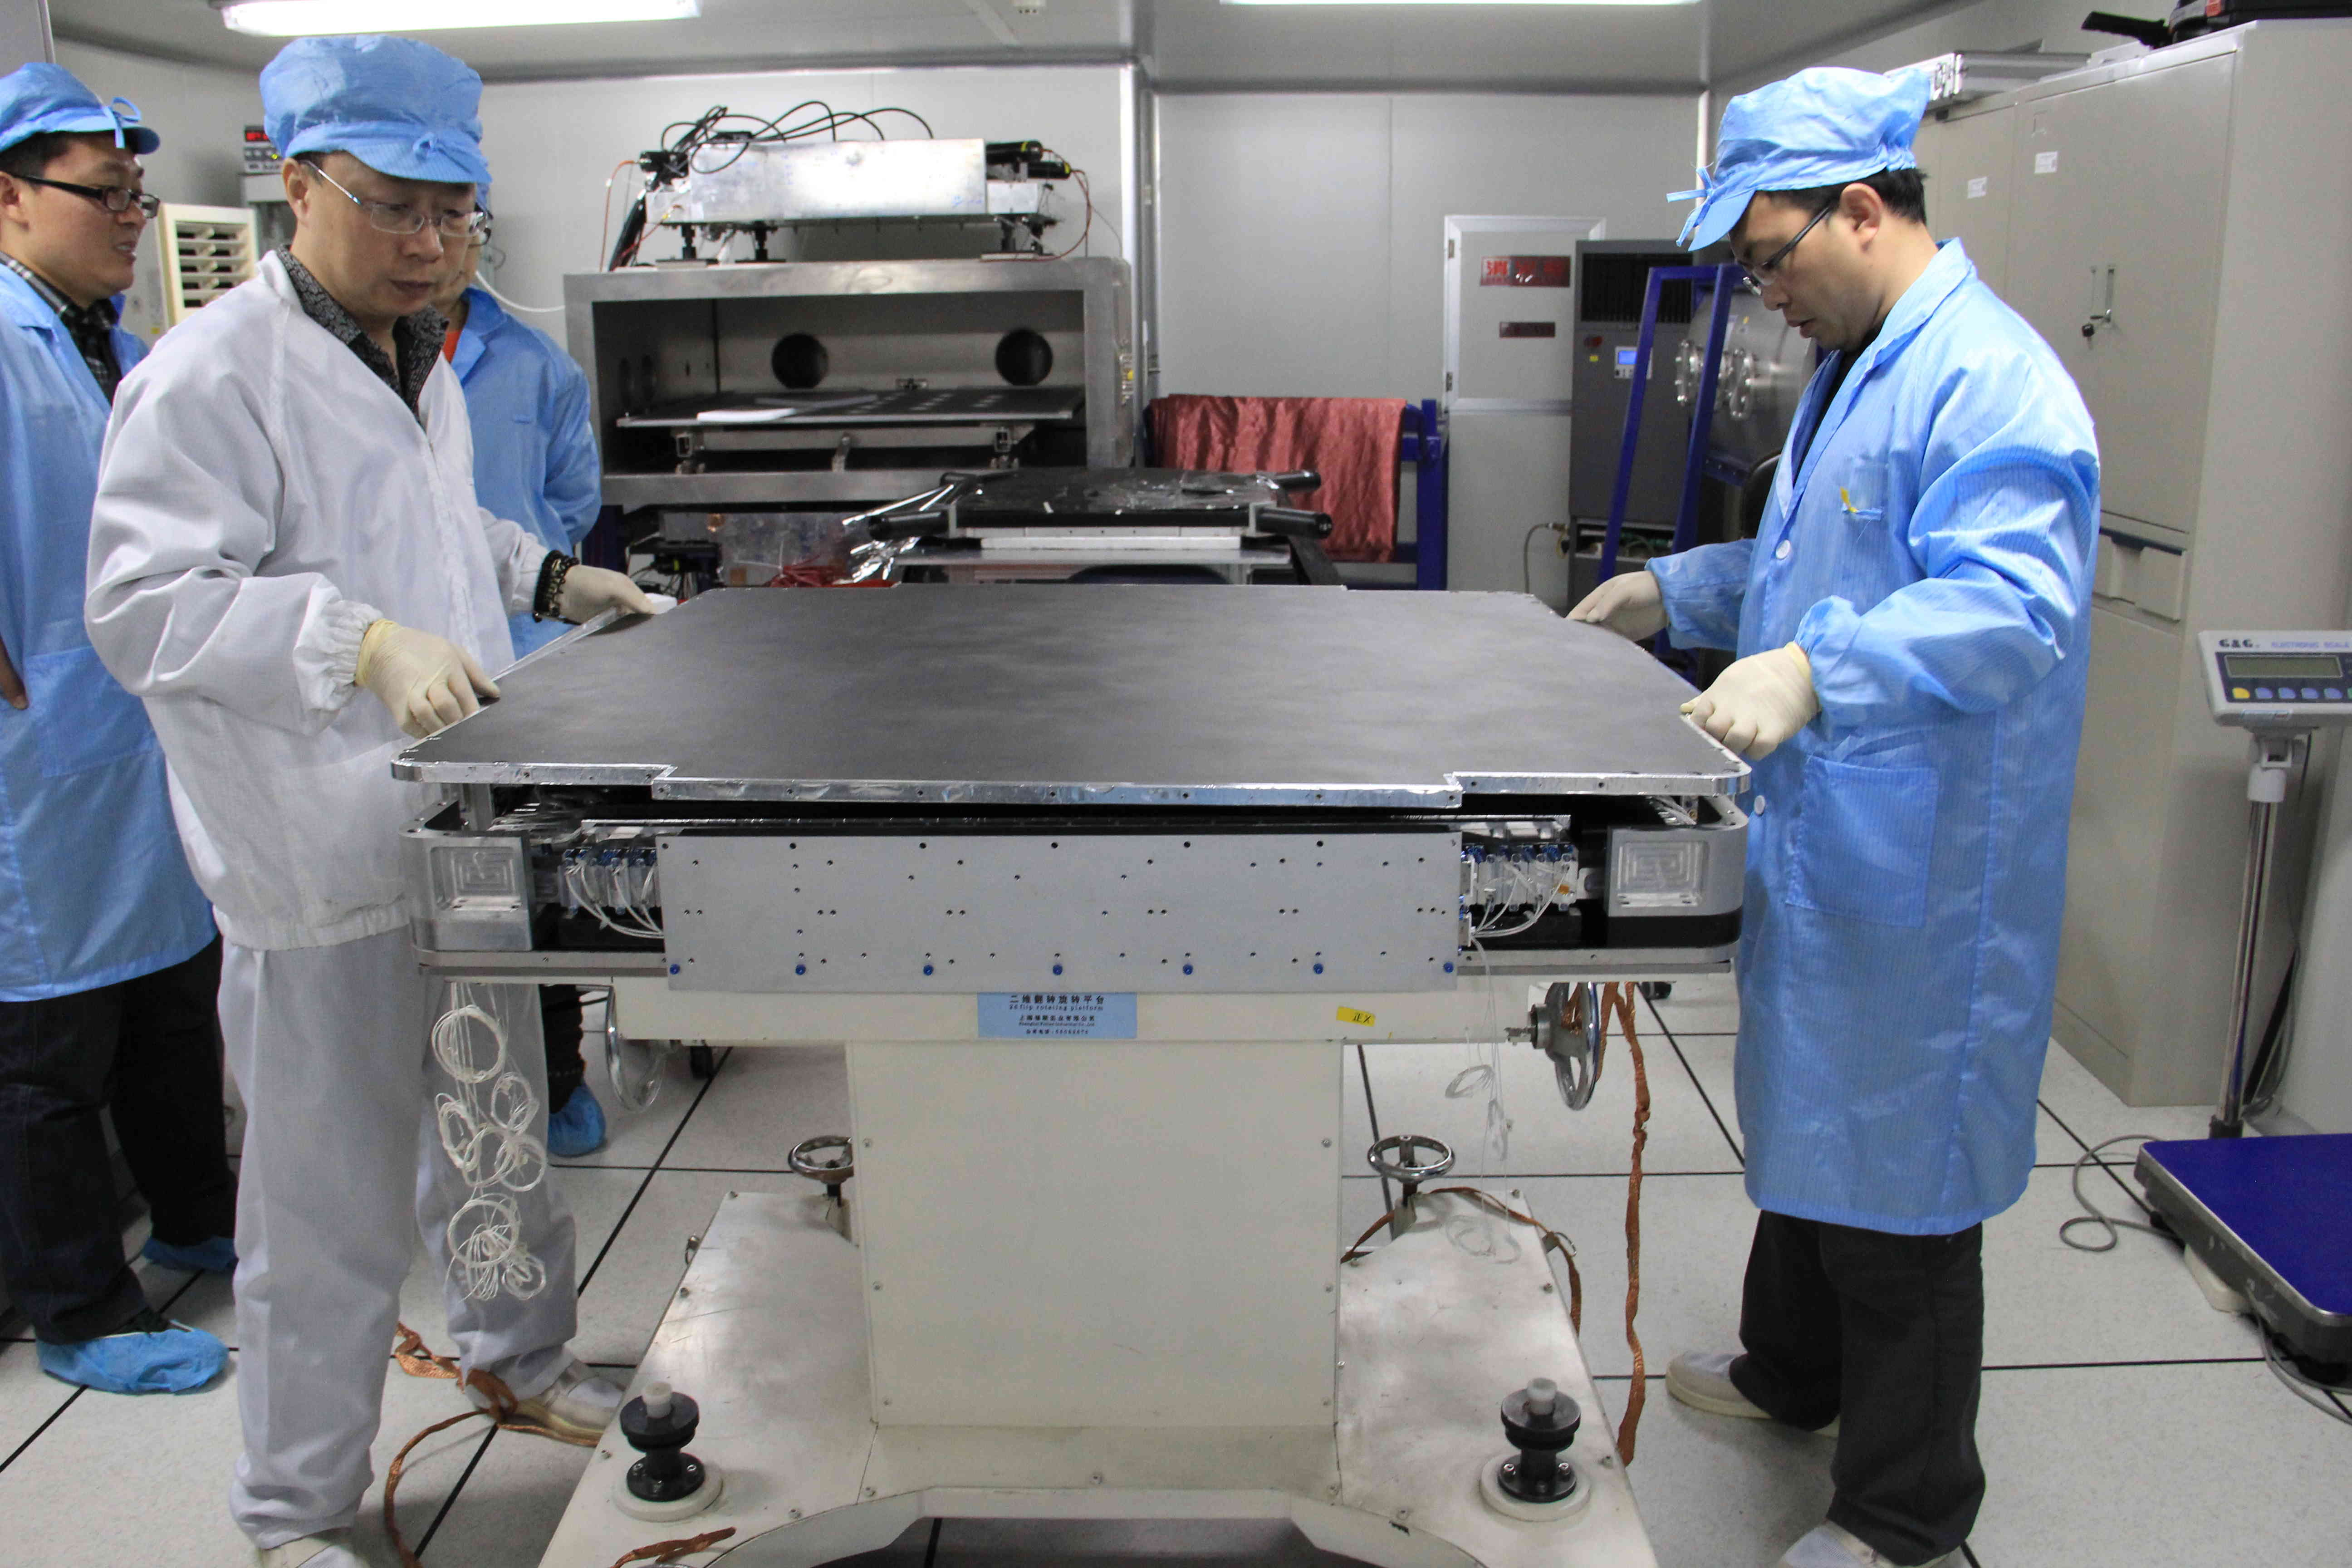
\includegraphics[width=0.33\textwidth]{chap/construction/fig/assembly_f.jpg}
}
\caption{PSD的整体装配步骤}
\label{fig:construction:psd_assembly}
\end{figure}
%
\begin{enumerate}[label={\alph*)}]
	\item 布置金属导电胶带。这是为了将整个PSD结构地连接在一起,以提高PSD的抗电磁干扰能力,降低基线噪声展宽。
	\item 安装塑闪单元条组件。两个探测平面,共4层塑闪单元条组件,逐层进行安装。安装时先固定该方向上的两组梁结构,然后将单元条逐一安装到对应的底板或盖板条形凹槽中,其位置由铝合金梁结构上的“工”型凹槽决定。
	\item 安装PMT组件。安装前,先在PMT组件的管体周围缠绕一层玻莫合金,然后将PMT组件轻轻推进梁结构上的PMT孔洞。PMT组件位置调整合适后,再将其上的铝合金保护套用螺丝固定到梁结构上。为了确定PMT组件在安装过程中没有受到损伤以及确定PMT与塑闪单元条的耦合是否正常,在PMT组件安装完成后,进行下一步安装操作前,我们给每个PMT组件加上额定工作电压,使用宇宙线对其进行功能完整性检测。由于塑闪单元条组件也已经安装,此时可以得到各个单元模块的MIP响应,结果如图\ref{fig:construction:mipVSstrip}所示。图中将同一探测平面两端的结果综合在了一起,正端在下,负端在上,其中横轴是该探测平面内的探测单元模块编号,纵轴是减去基线的原始ADC道数。可以看到,所有模块都能够正常工作,而且各模块间具有较好的能量响应一致性。
	\begin{figure}[htbp]
	\centering
	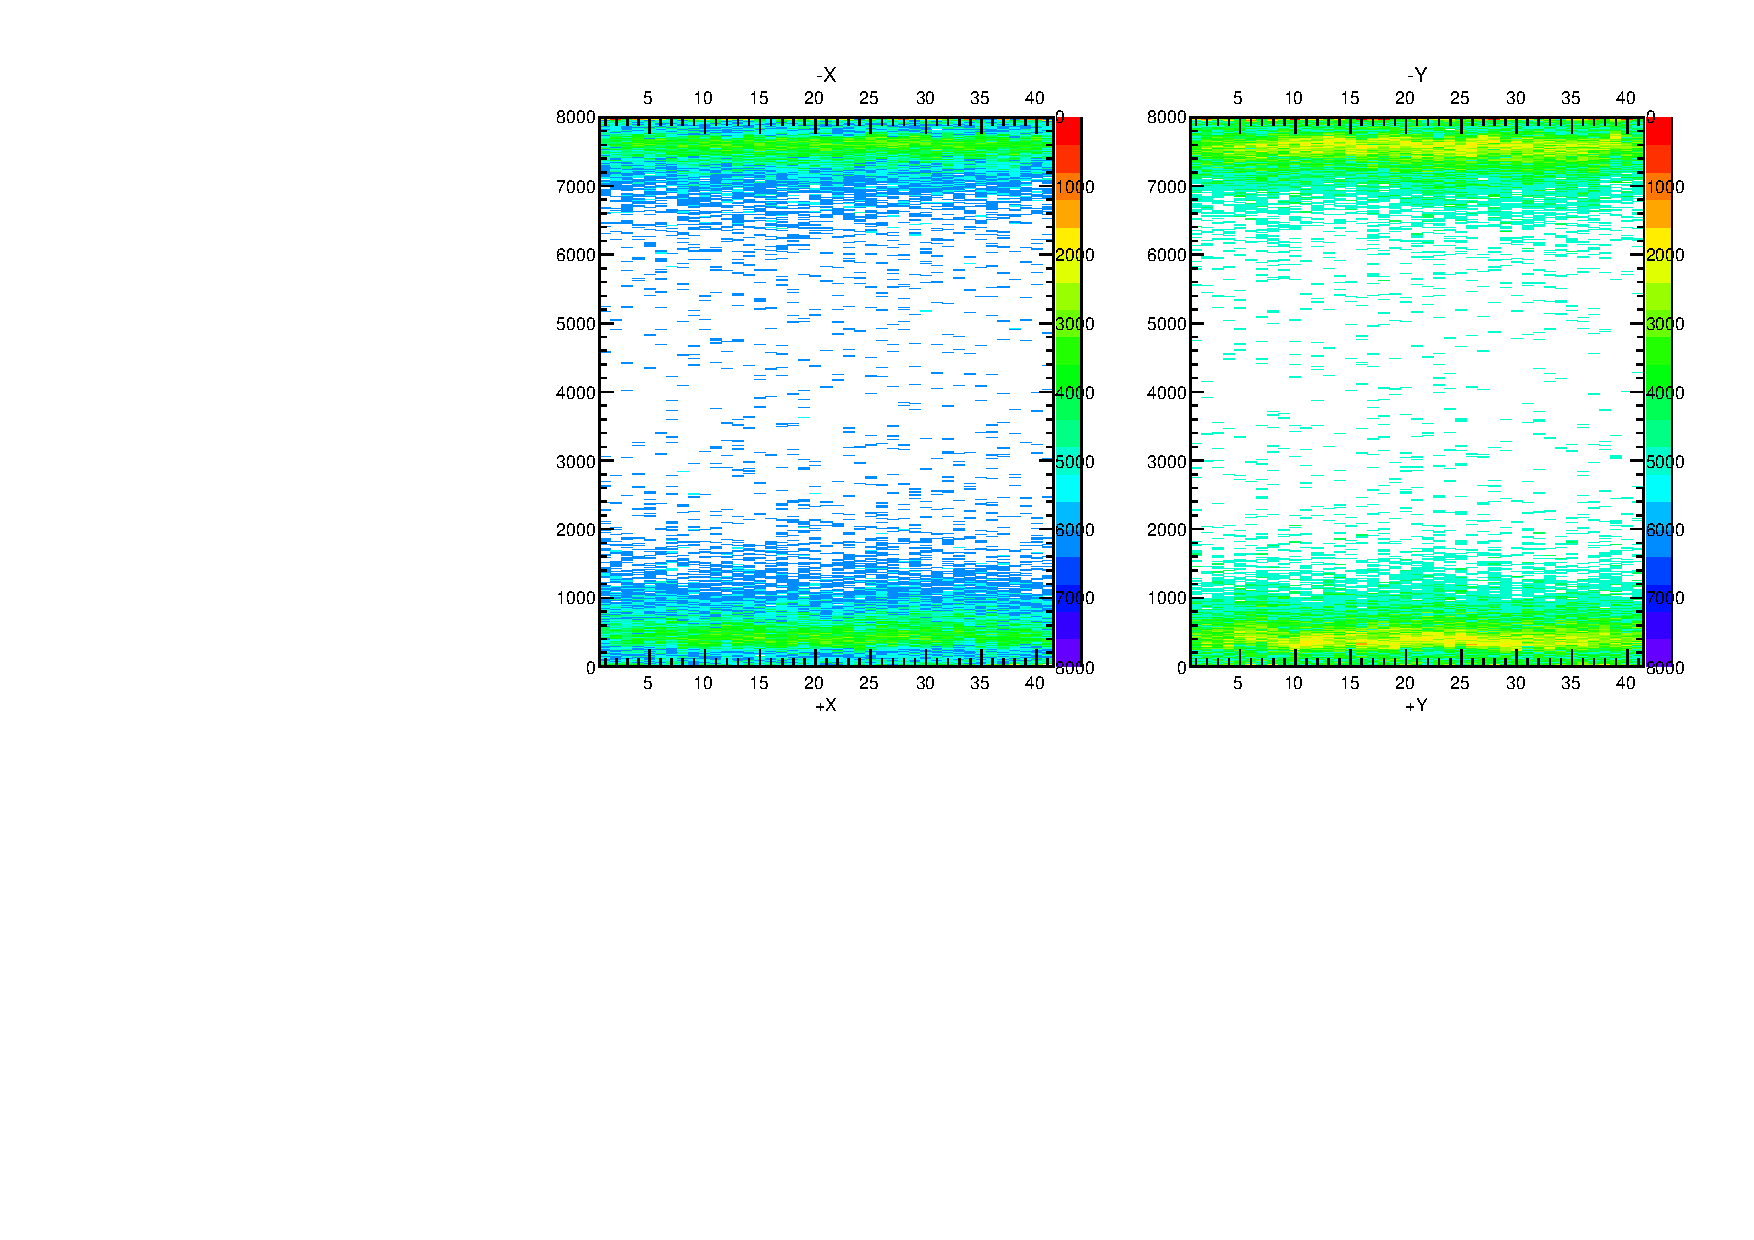
\includegraphics[width=0.6\textwidth,angle=-90]{chap/construction/fig/mipVSstrip.pdf}
	\caption{塑闪单元条与PMT组件全部安装到位后的宇宙线检测结果}
	\label{fig:construction:mipVSstrip}
	\end{figure}

	\begin{figure}[htbp]
	\centering
	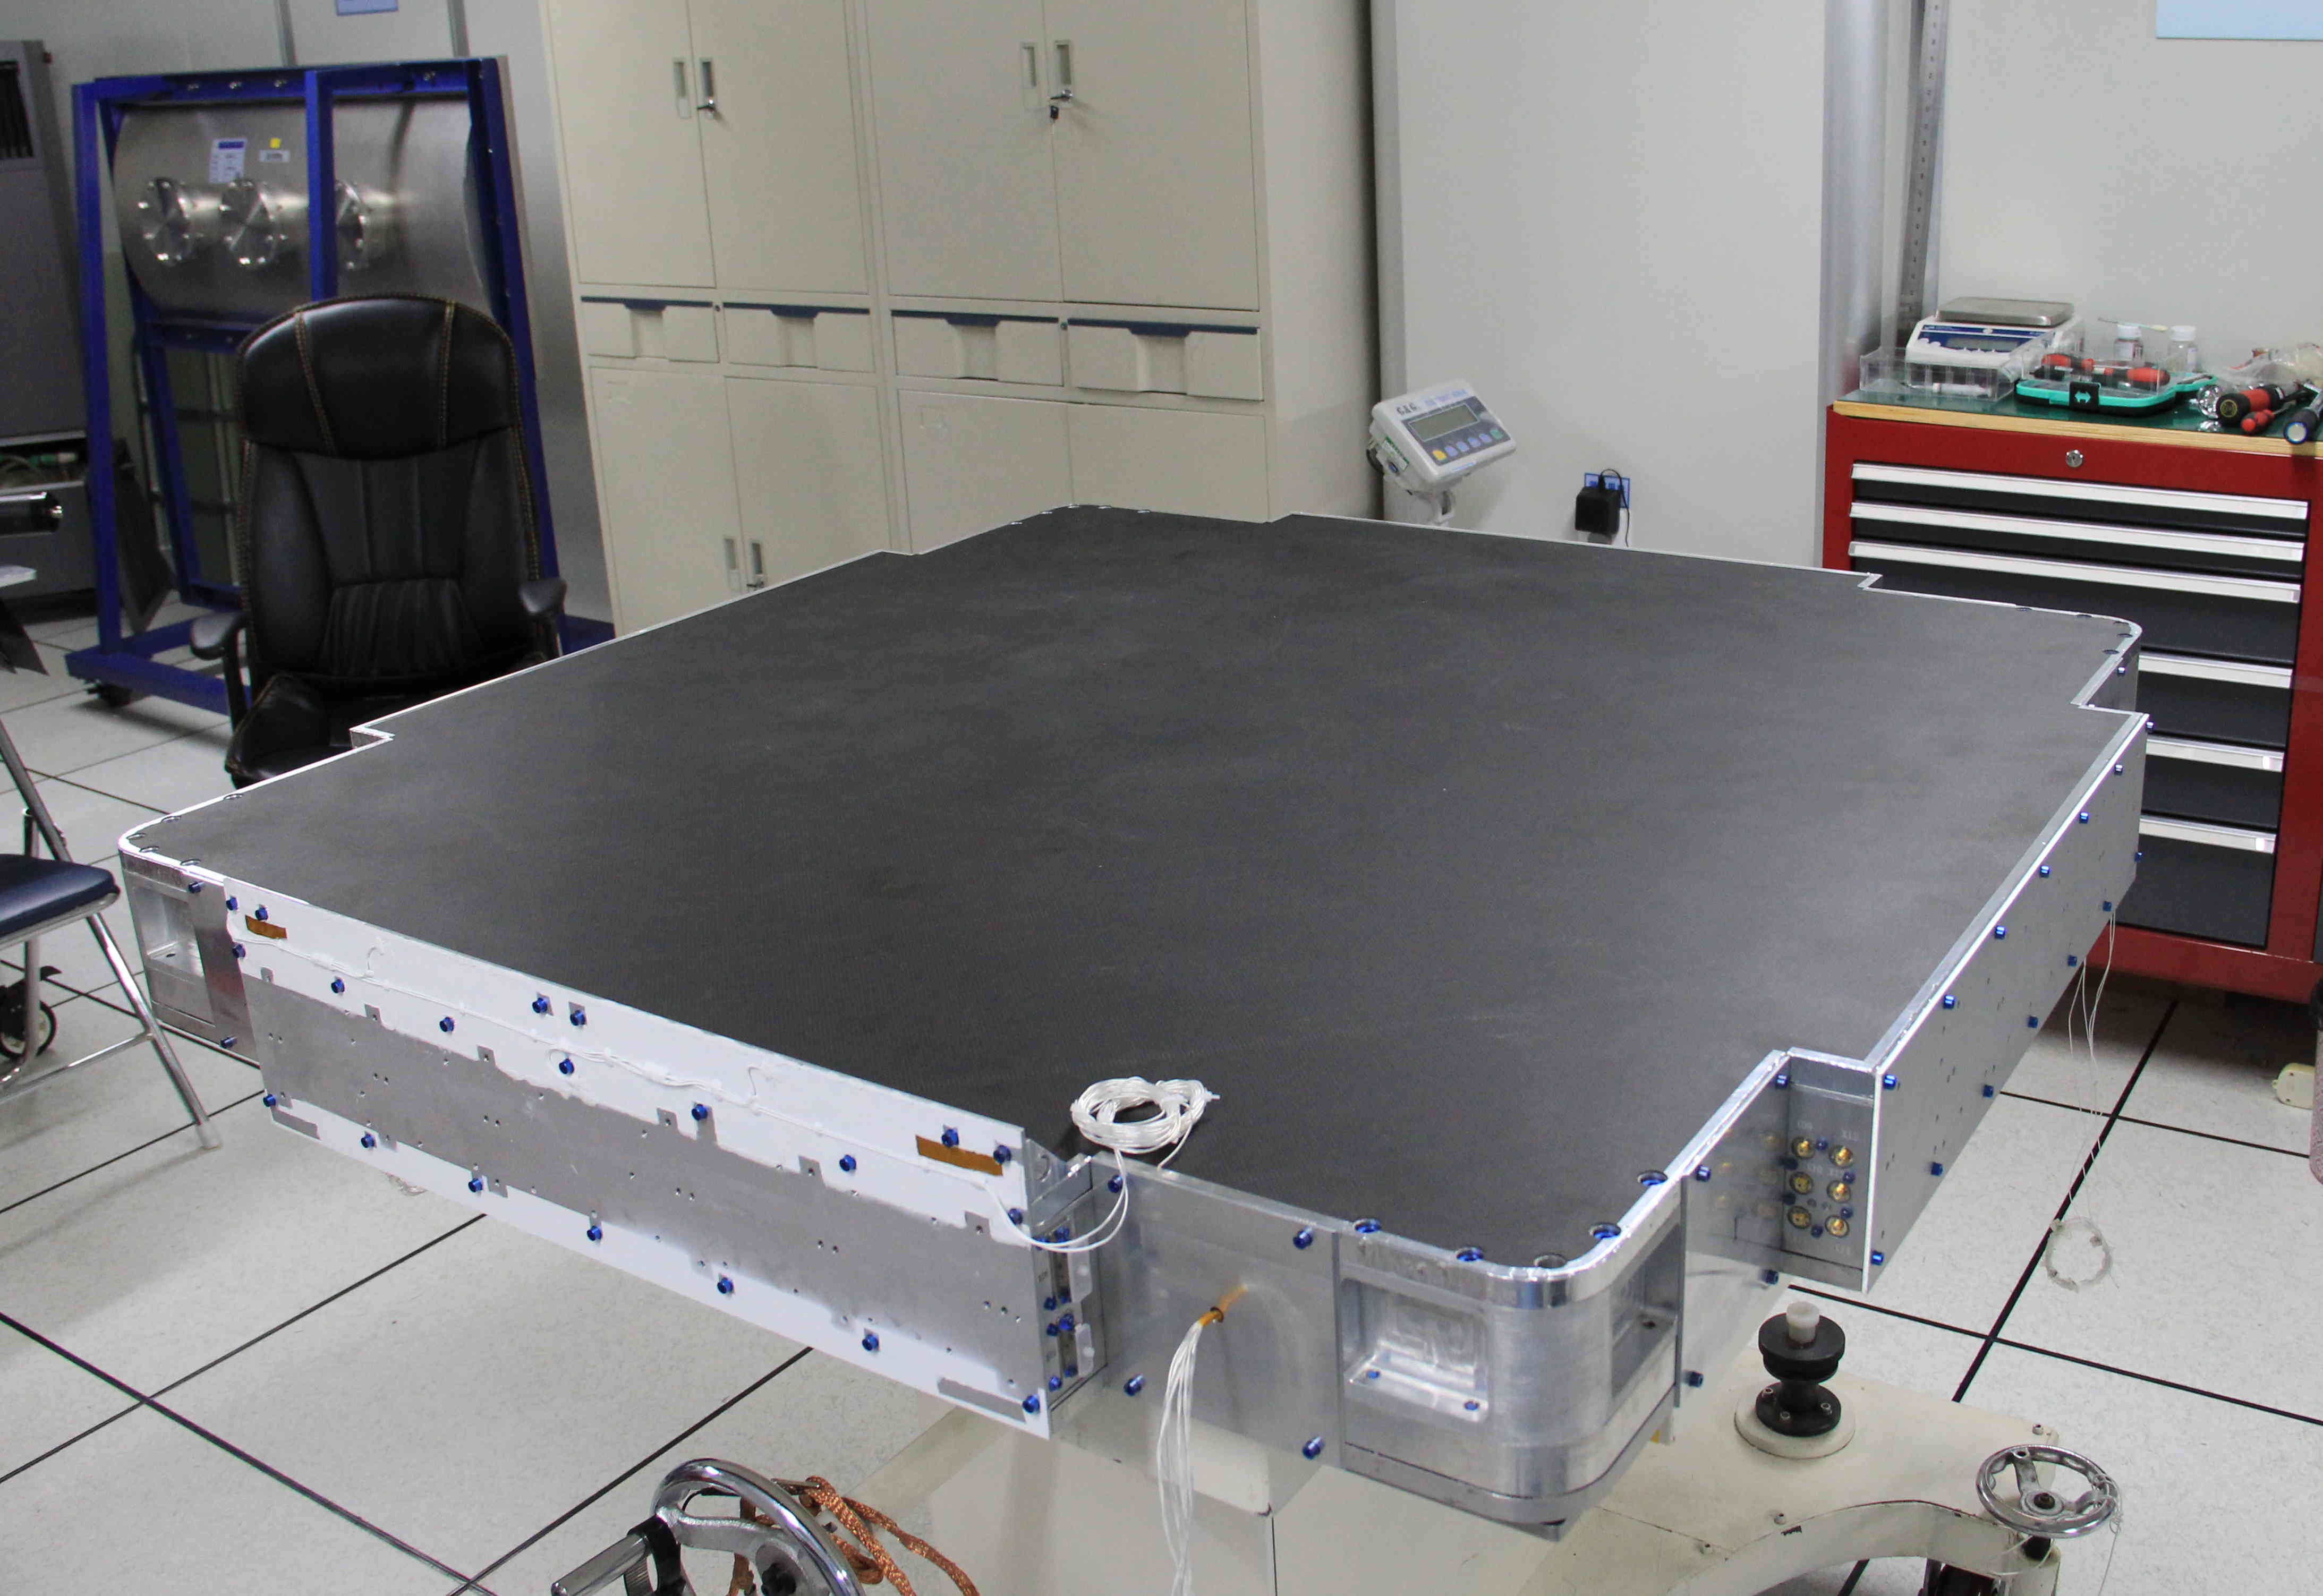
\includegraphics[width=0.65\textwidth]{chap/construction/fig/psd.jpg}
	\caption{PSD整体装配完成后的样子}
	\label{fig:construction:psd}
	\end{figure}

	\item 电装。主要是将PMT组件上的高压线和信号线分别焊接到高压扇出板和信号转接板上,焊接工作由来自山东航天电子技术研究所的专业人员完成。
	\item 安装FEE机箱。FEE机箱是前端电子学板、信号转接板以及高压扇出板的载体。这一步主要是将前端电子学板和信号转接板连接在一起,并固定FEE机箱。
	\item 封顶。主要是安装顶部盖板以及四周的角板,完成PSD整体的密封,这是PSD总装的最后一步。
\end{enumerate}
PSD整体装配完成后的最终外观如图\ref{fig:construction:psd}所示。
